%%
%% This is file `mcmthesis-demo.tex',
%% generated with the docstrip utility.
%%
%% The original source files were:
%%
%% mcmthesis.dtx  (with options: `demo')
%%
%% -----------------------------------
%%
%% This is a generated file.
%%
%% Copyright (C)
%%     2010 -- 2015 by Zhaoli Wang
%%     2014 -- 2016 by Liam Huang
%%     2016 -- 2018 by Xuehan Sun
%%
%% This work may be distributed and/or modified under the
%% conditions of the LaTeX Project Public License, either version 1.3
%% of this license or (at your option) any later version.
%%
%% This work has the LPPL maintenance status `maintained'.
%%
%% The Current Maintainer of this work is Xuehan Sun.
%%
\documentclass[12pt]{mcmthesis}
\mcmsetup{CTeX = false,   % 使用 CTeX 套装时,设置为 true
        tcn = 053, problem = A,
        sheet = true, titleinsheet = true, keywordsinsheet = true,
        titlepage = true}
\usepackage{palatino}
\usepackage[
    style = ieee,
    maxnames = 4
    ]{biblatex}
\usepackage{mwe}
\usepackage{caption}
\usepackage{graphicx}
\usepackage{subcaption}
\usepackage{float}
\usepackage{multirow}
\usepackage{indentfirst}
\usepackage{gensymb}
\usepackage{url}
\usepackage[ruled,lined,commentsnumbered]{algorithm2e}
\usepackage{geometry}
\geometry{left=2cm,right=2cm,top=2cm,bottom=2cm} %%页边距


\addbibresource{bib/thesis.bib}


\begin{document}

\linespread{0.6} %%行间距
\setlength{\parskip}{0.5\baselineskip} %%段间距
\title{MoC-SEIR: Analysis of the Epidemic Situation of 2019-nCoV with Various Factors}

\date{\today}
	\begin{abstract}
	
The coronavirus ignites a fast-growing outbreak in China. To date, the death toll in China has risen to 811, surpassing the death toll from the SARS epidemic of 2002-3, according to official data released early on the morning of Feb. 9.

To assist the Chinese Center for Disease Control and Prevention (China CDC) better in decision making, we build a \textbf{modified compartmental SEIR model (MoC-SEIR)} in search for potential demographic trend of infection. Infectious disease model is frequently used to simulate the spread of disease. Given some characteristics of the coronavirus including an averaged 7-day incubation period and relative low fatality rate compared to SARS, we choose \textbf{SEIR} as the basis of our model among all mathematical models of epidemic disease.

Since the virus originated in Wuhan, We divide the regions into three groups, Wuhan, Hubei without Wuhan and Mainland China ignoring the Hubei, with different parameters in model. The raw SEIR does not explain well about the data we collected. So we take population flow and travel limitations into our model, which yields more satisfactory results. \textbf{The basic reproductive number of the virus is 3.15} calculated based on our parameters. We also make some predictions about how the trend will develop. A decrease in number of infections is expected around Feb. 18. We also build a model on a global scale. \textbf{Grey Verhulst model} is introduced to forecast oversea infections as little information about the foreign cases is disclosed, suggesting the spread trend has been stemmed abroad. That is to say, the virus would not cause too much trouble for other countries.

Based on our model, we analyze and quantify the impacts of measures taken by the Chinese government. The imposed travel limitations has greatly blunted the outbreak's impact and prevented a broader outbreak. The extended holidays postponed the huge population reflow which could bring devastating damage to the city when the virus is highly contagious. But \textbf{the coin has two sides}. The abrupt lockdown in a way overstretched the hospitals in Wuhan, which borne most brunt of the epidemic. The disaster also put tertiary industry and industrial production under severe strain.

Besides, we introduce various factors into our model. \textbf{Secondary infection, emergence of effective treatment and returning after Spring Festival} are reasonable expectations in the development of the outbreak. We consider their influence on the development of the outbreak respectively. Given the prediction on the global trend, we have every reason to believe that World Health Organization(WHO) will terminate the PHEIC by \textbf{the end of March}. In the last analysis, we test the stability of model and present both strengths and weaknesses.

Measures, in either personal or national perspective, are fully discussed, which might reduce the chance of virus spread between individuals. In future works, we hope to dive into the subtle influences of exposers and population variation.
	
		\begin{keywords}
		 2019-nCoV; SEIR Model; Grey Verhulst; Population Flow; Control Measure
		\end{keywords}
	\end{abstract}

\maketitle

\tableofcontents

\newpage

\section{Introduction}

\subsection{Background}
An outbreak of a pneumonia-like illness that started in the Chinese city of Wuhan has put health authorities on high alert around the world. The novel coronavirus was officially named as 2019-nCoV, which was identified as the causative virus for the acute respiratory disease on 7 January 2020. It has led cities to lockdown, cancellation of flights to and from China and disruption in global business. It takes a toll on all aspects of people's life. The WHO declared a global emergency on Jan. 30 as the illness continued to spread.

\begin{figure}[h]
    \centering
    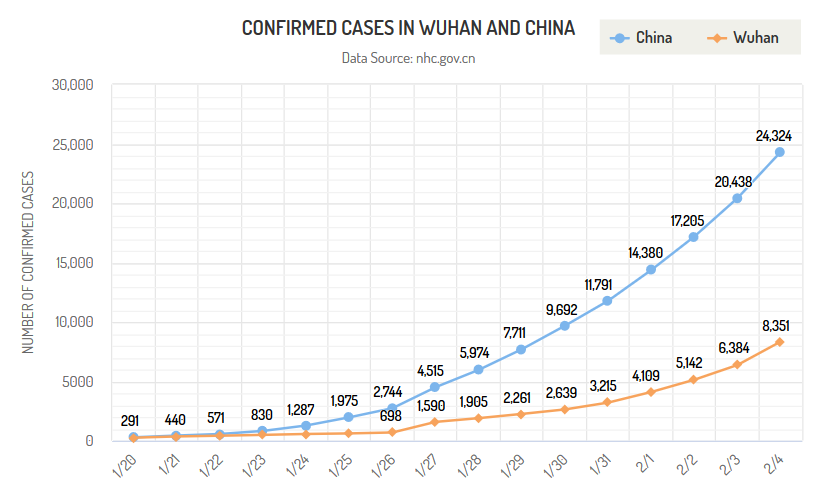
\includegraphics[width=0.8\textwidth]{figure/Confirmed_Cases.png}
    \caption{Confirmed Cases in Wuhan and China}
    \label{fig:Conf_Cases}
\end{figure}

However, as there exists a one-week incubation period for the infected on average, massive people have unconsciously exposed to virus carriers and then travelled to other places before the widespread outbreak. Although the Chinese government takes powerful measures in a short time, trying to prevent the epidemic situation from worsening, how to control the trend of outbreak development effectively still becomes an intractable problem.

\subsection{Related work}
Since the abrupt increase in the number of 2019-nCoV infections in China, much attention has been paid to the research on its trend and prevention. Many teams estimated the reproductive number of the virus based on the preliminary statistics, such as 3.11 by J. M. Read, \textit{et al.}~\cite{early_est}, 2.24 to 3.58 by Shi Zhao, \textit{et al.}~\cite{pre_est} and so on. Some efforts have been made looking into the taken and future control measures of the Chinese government, including travel restrictions, holiday extension etc. Tang Biao et al. worked on how travel restriction would limit the spread in Beijing~\cite{trans_risk} and Ai Siqi et al. explored the relation between the number of cases and the timing of city closure policy~\cite{city_closure}.

Up to the present, most articles build their models for a certain region, but few work constructs a systematic mathematical model to describe the interzone spread of 2019-nCoV, which is the main purpose of our attempt in this paper.

\subsection{Our Work}
In summary, our work addresses three primary problems:
\begin{enumerate}
    \item According to current reports and statistics on the appraisal of the epidemic, we build a compartmental model based on the SEIR~\cite{SI_model_origin} proposed by Kermack et al. to predict the spread trend of 2019-nCoV. Our model fits the collected data well and gives a reasonable prediction of both domestic and global infections in the next period of time.
    \item As traditional transportation brings a sudden and significant increase to the intensity of population flow, we quantify its influence based on epidemiology, either with or without the prevention and control measures by Chinese government, and thus explain the positive and negative effects of those measures.
    \item Based on our prediction model, we list some factors closely related to the development of epidemic situation and analyze their impact in the next two months. We also show that WHO will terminate the PHEIC in the end of March. 
\end{enumerate}

In Section 2, we state the basic assumptions of our model. Section 3 contains the nomenclature used for model description. Section 4 presents our modeling process and result. The characteristics of our model and the sufficient condition of high parameter sensitivity are discussed in Section 5 and some trains of thought against the spread of virus are proposed in Section 6. Finally, we conclude our paper in Section 7.

\section{Assumptions and Justifications}
Given current evidence and reports, our model makes the following assumptions:
\begin{itemize}
    \item \textbf{Virus carrier flows except those out from Wuhan are ignored.} According to our collected data, most victims of the virus got infected in Wuhan and the infection ratio in other regions is much lower. When considering the influence of population flows on the epidemic situation, only those from Wuhan to the rest of provinces make a significant difference.
    \item \textbf{The total population of any region is considered constant.} Birth and death are omitted when considering the total population. On one hand, we have few access to the detailed statistics of population flows and birth/death rate of a certain region. On the other hand, all of them make little difference to the spread of virus.
    \item \textbf{The incubation period is a random variable with exponential distribution with parameter $\theta$.} The Exposed developed into infectious ones at a proportion of $\theta$.
    \item \textbf{There is no outflow of population in Hubei once the extreme control measures are taken,} which means virus transfer among provinces is suppressed entirely. So we do not consider imported cases in this stage. 
    \item \textbf{The infections brought by exposers are neglected.} Although it's reported that exposers are also able to spread the virus, their spread ability is relatively much weaker than the infected ones and thus does not make significant difference to the epidemic situation.
    \item \textbf{The mutation speed of virus is relatively slow.} The cured individuals are immune to the virus. As for task 3, we will consider the scenario of secondary infection.
\end{itemize}

\section{Nomenclature}
Here are some notations to clarify before we introduce our work. The meaning of the superscript is also shown in table \ref{tab:Nomen}.

\linespread{1.0}
\begin{table}[H]
    \centering
    \caption{Nomenclature}
    \label{tab:Nomen}
    \begin{tabular}{p{4cm}p{10cm}}
    \hline
    Notation & Definition \\
    
    \hline
    $D$ & Death toll \\
    $R$ & Individuals having recovered from infection \\
    $I$ & Infected individuals \\
    $C$ & Confirmed cases  \\
    $E$ & Exposed individuals \\
    $S$ & Susceptible individuals \\
    $P$ & The total population of a region \\
    $F$ & The flowing population of a region \\
    $\theta$ & The reciprocal of incubation period \\
    $f_{t,o}$ & The ratio of outflow population from a region at $t$ \\
    $f_{t,i}$ & The ratio of inflow population to a regions at $t$ \\
    $f^{(0)}$ & $f_{out}$ or $f_{in}$ of Wuhan \\
    $f^{(1)}$ & $f_{out}$ or $f_{in}$ of other regions in Hubei \\
    $f^{(2)}$ & $f_{out}$ or $f_{in}$ of other regions outside Hubei in China \\
    
    \hline
    \end{tabular}
    \label{tab:notation}
\end{table}
\linespread{0.6}

\section{Modeling} \label{Sec:Modeling}
\subsection{Data Collection}

To have a better insight into this outbreak and simulate our model, we first collected the number of confirmed cases from a GitHub repository~\cite{data_github}. We organize the data in a temporal-spatial order to facilitate our training. Most provinces declared its first confirmed case around Jan. 22. Therefore, our data for these regions ranges from Jan. 22 to Feb. 4. However, since the virus originate from Wuhan in Hubei province, more data can be acquired from Hubei government official sites compared to other provinces. So more previous data has been collected for Hubei.

\subsection{MoC-SEIR: Modified Compartmental SEIR Model}

Compared with common infectious diseases, we find nCoV is a bit different in that carriers are likely to spread it even during incubation period when carriers might show similar symptoms with those suffering from serious flu. The trait makes it harder to distinguish between the positive and negative ones. It also translates into the soaring potentially infected population flowing out. Therefore, we modify the classic SEIR model so that it can fit current situation more precisely. In our modified SEIR model, each member of the population typically progresses from susceptible to exposed, then to infectious and finally to recovered or dead. The whole process is illustrated in the flow diagram Figure \ref{fig:SEIR}, in which the boxes represent the different compartments and the arrows the transition between compartments.

\begin{figure}[H]
    \centering
    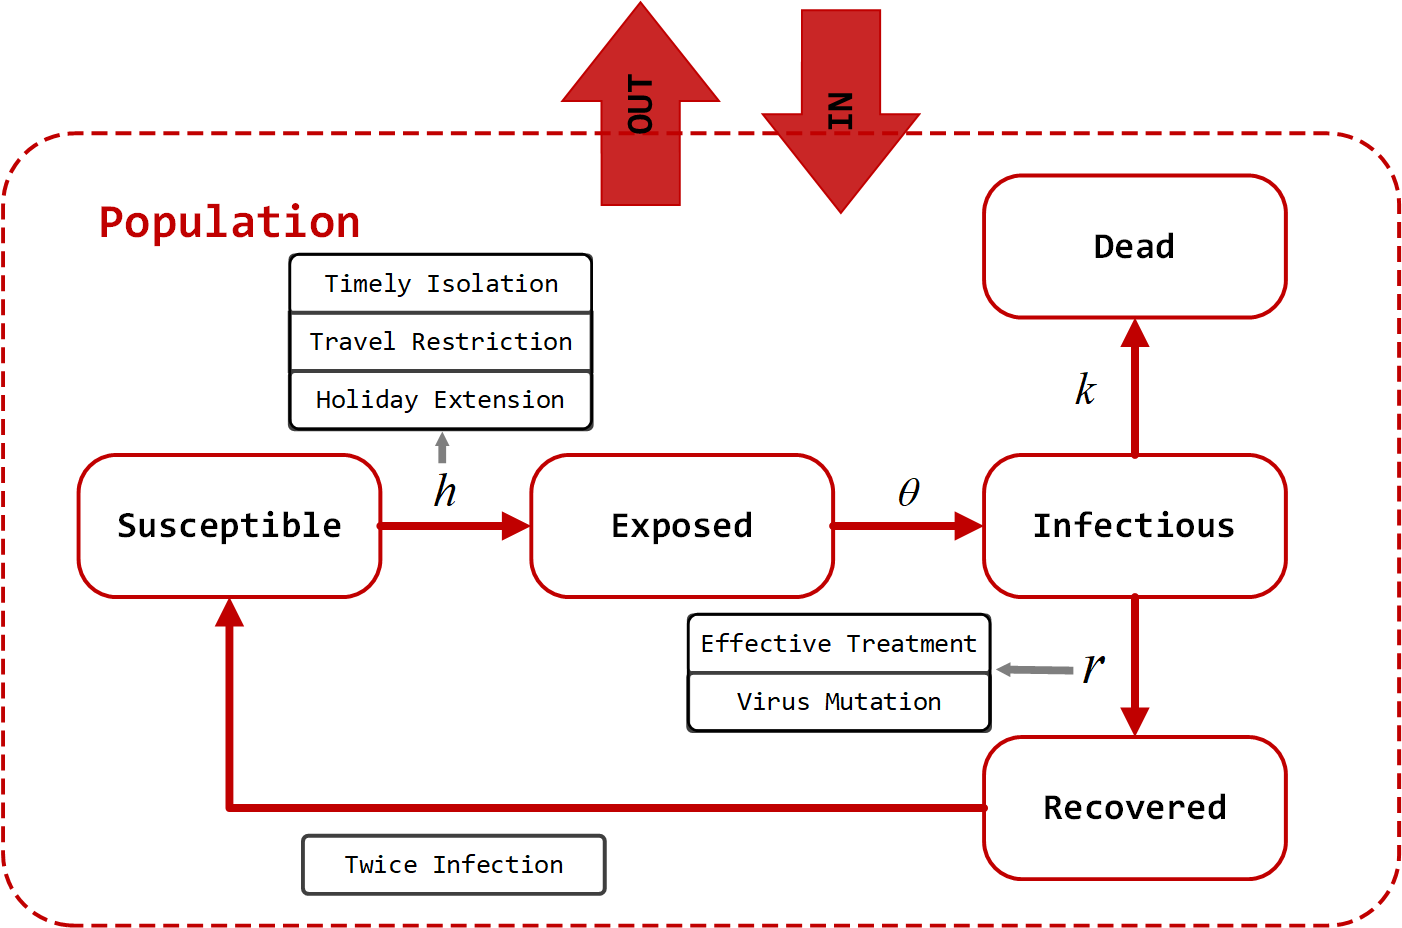
\includegraphics[width=0.9\textwidth,height=9cm]{053/figure/Flow_Chart.png}
    \caption{Modified Compartmental SEIR with Population Flow}
    \label{fig:SEIR}
\end{figure}

\subsubsection{Motivation}
Classic SEIR seems a satisfying model for the recent outbreak. It gives a curve of infections that grows exponentially in early stage and then levels off. However, given the known spread intensity of nCoV, we find that the curve has great deviation from the reported data in Wuhan, as shown in Figure~\ref{fig:noflow}. At the same time, we can hardly explain why countless infections have appeared in other regions of China without the idea of interzone population flows. In addition, it is obvious in Figure~\ref{fig:relation} that the number of confirmed cases is highly correlated $\left(r \approx 0.85\right)$ to the scale of inflow population from Wuhan. Therefore, we think it is necessary to introduce a variable to describe the effect of population flow.

\begin{figure}[htbp]
    \captionsetup{font={small}}
    \centering
    \begin{minipage}[c]{0.48\textwidth}
        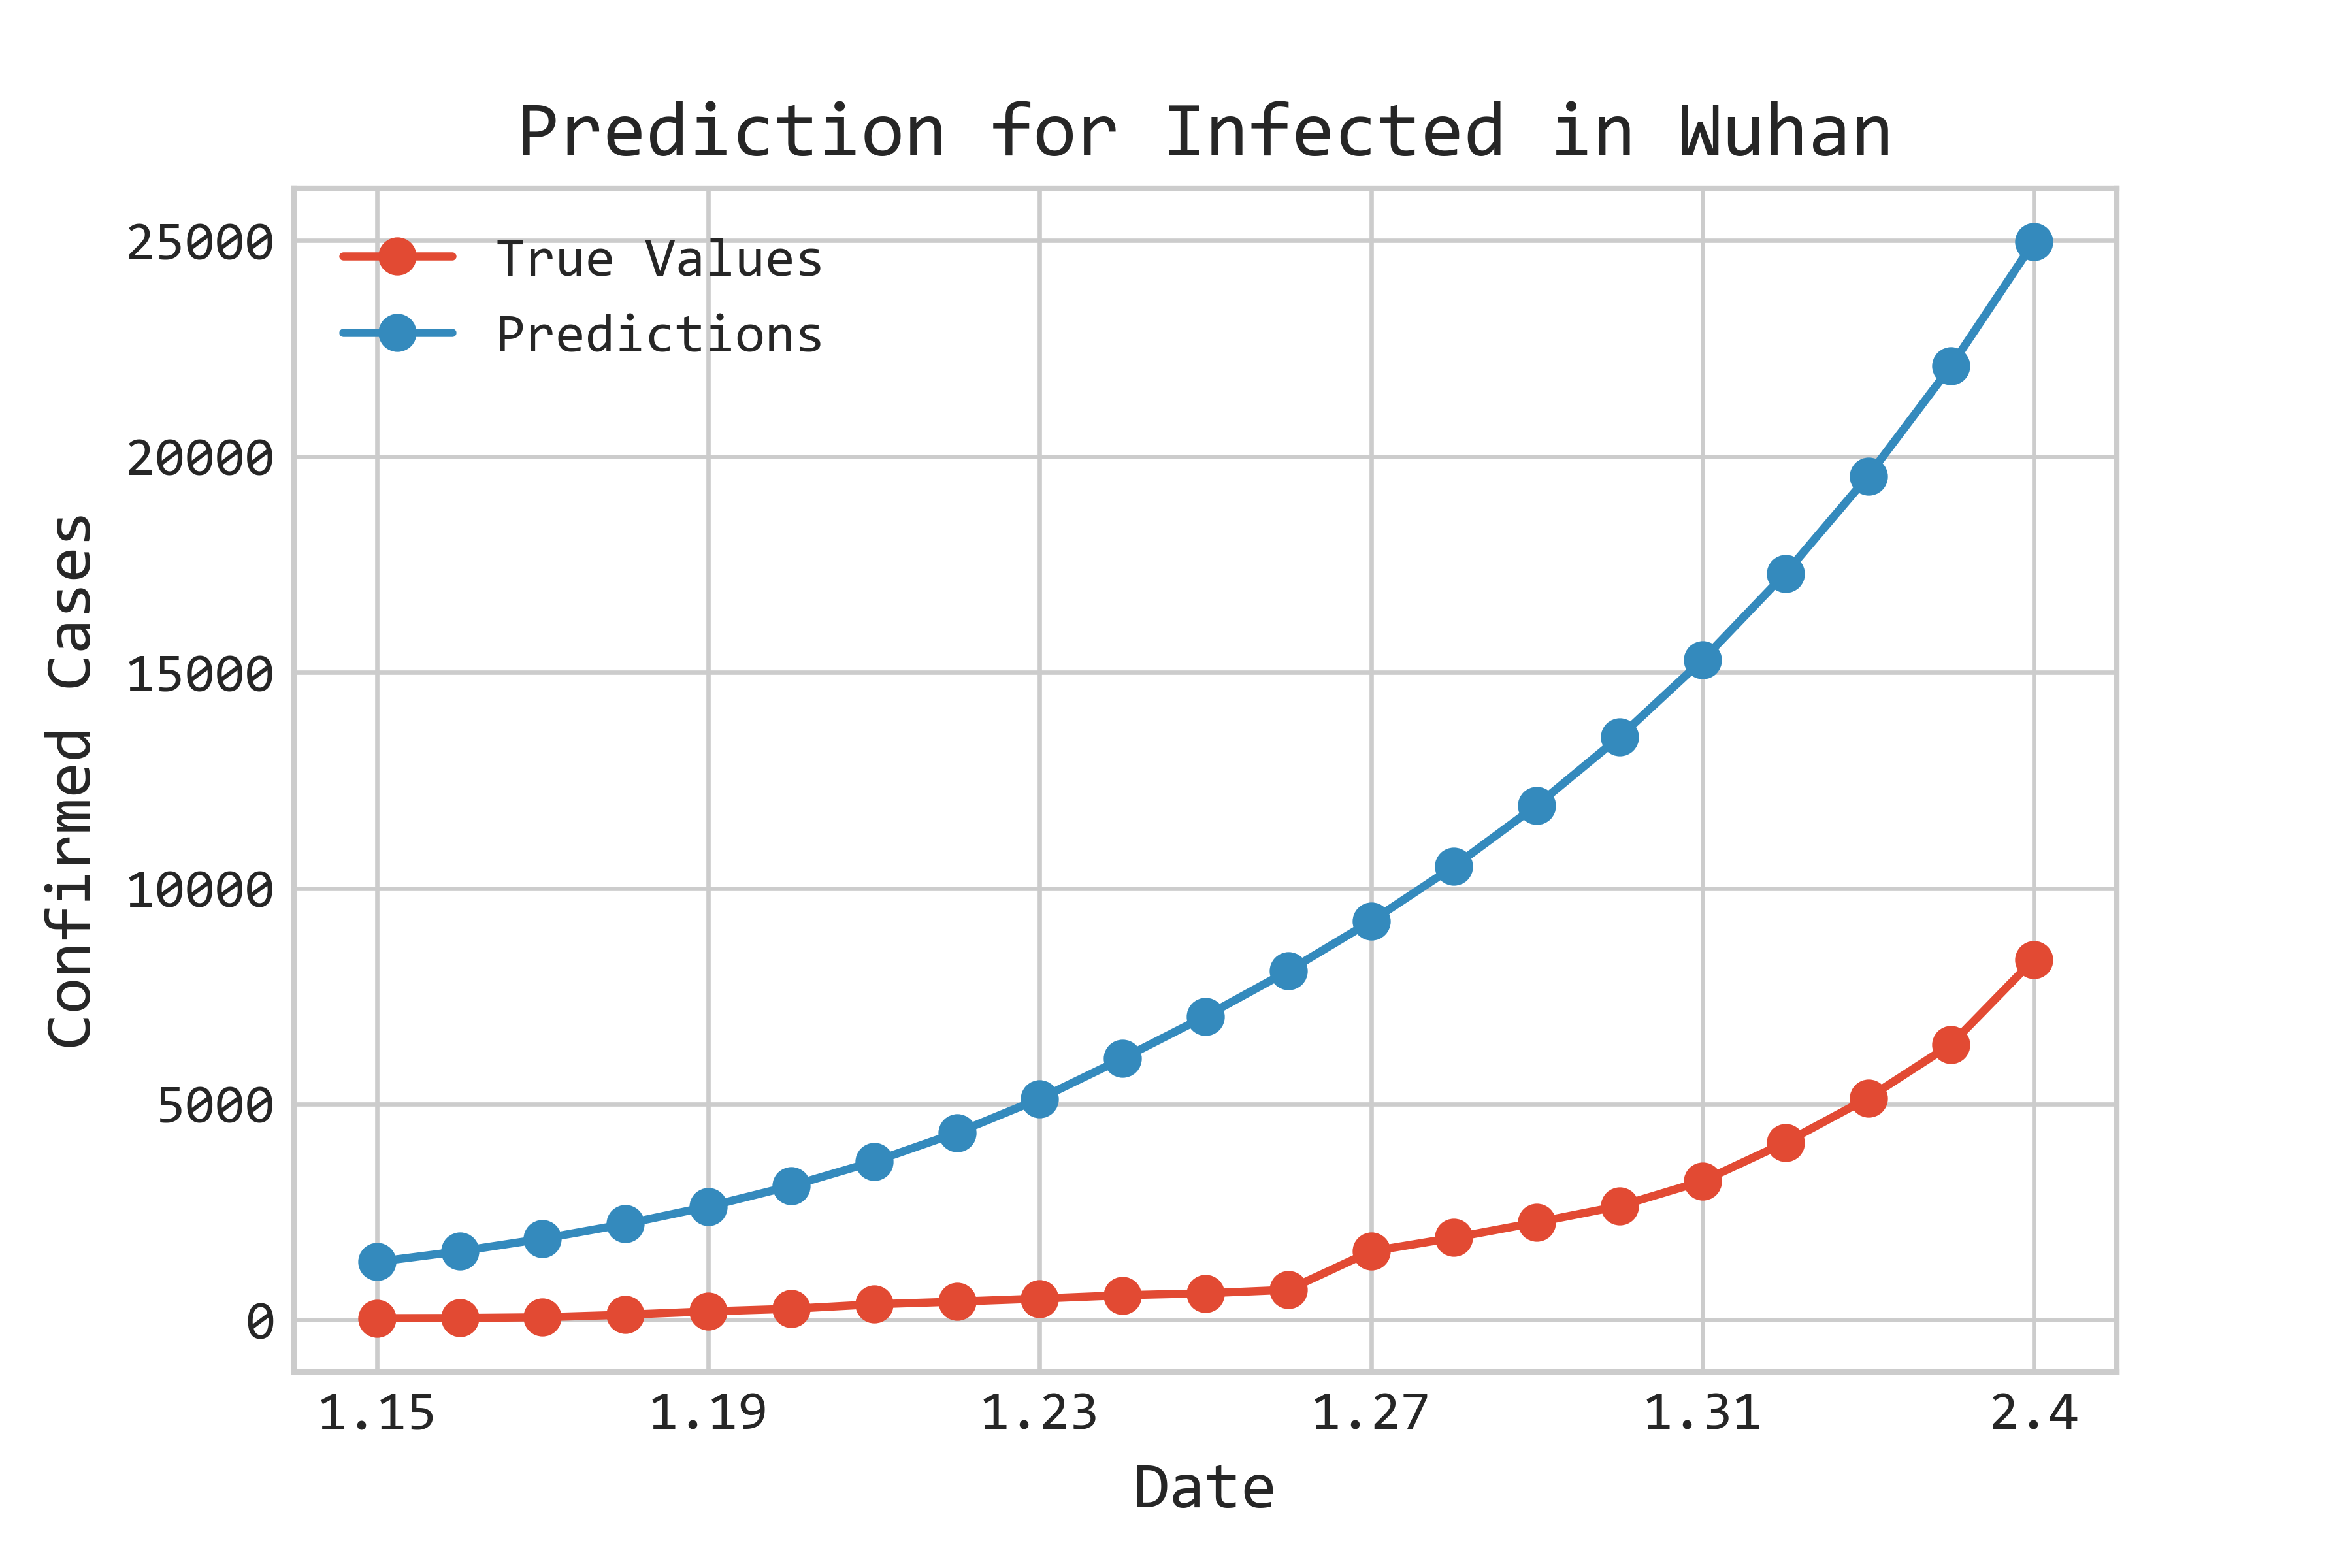
\includegraphics[width=1.0\textwidth]{figure/Wuhan_Naive.png}
        \caption{Curve Without Pop. Flow}
        \label{fig:noflow}
    \end{minipage}
    \begin{minipage}[c]{0.48\textwidth}
        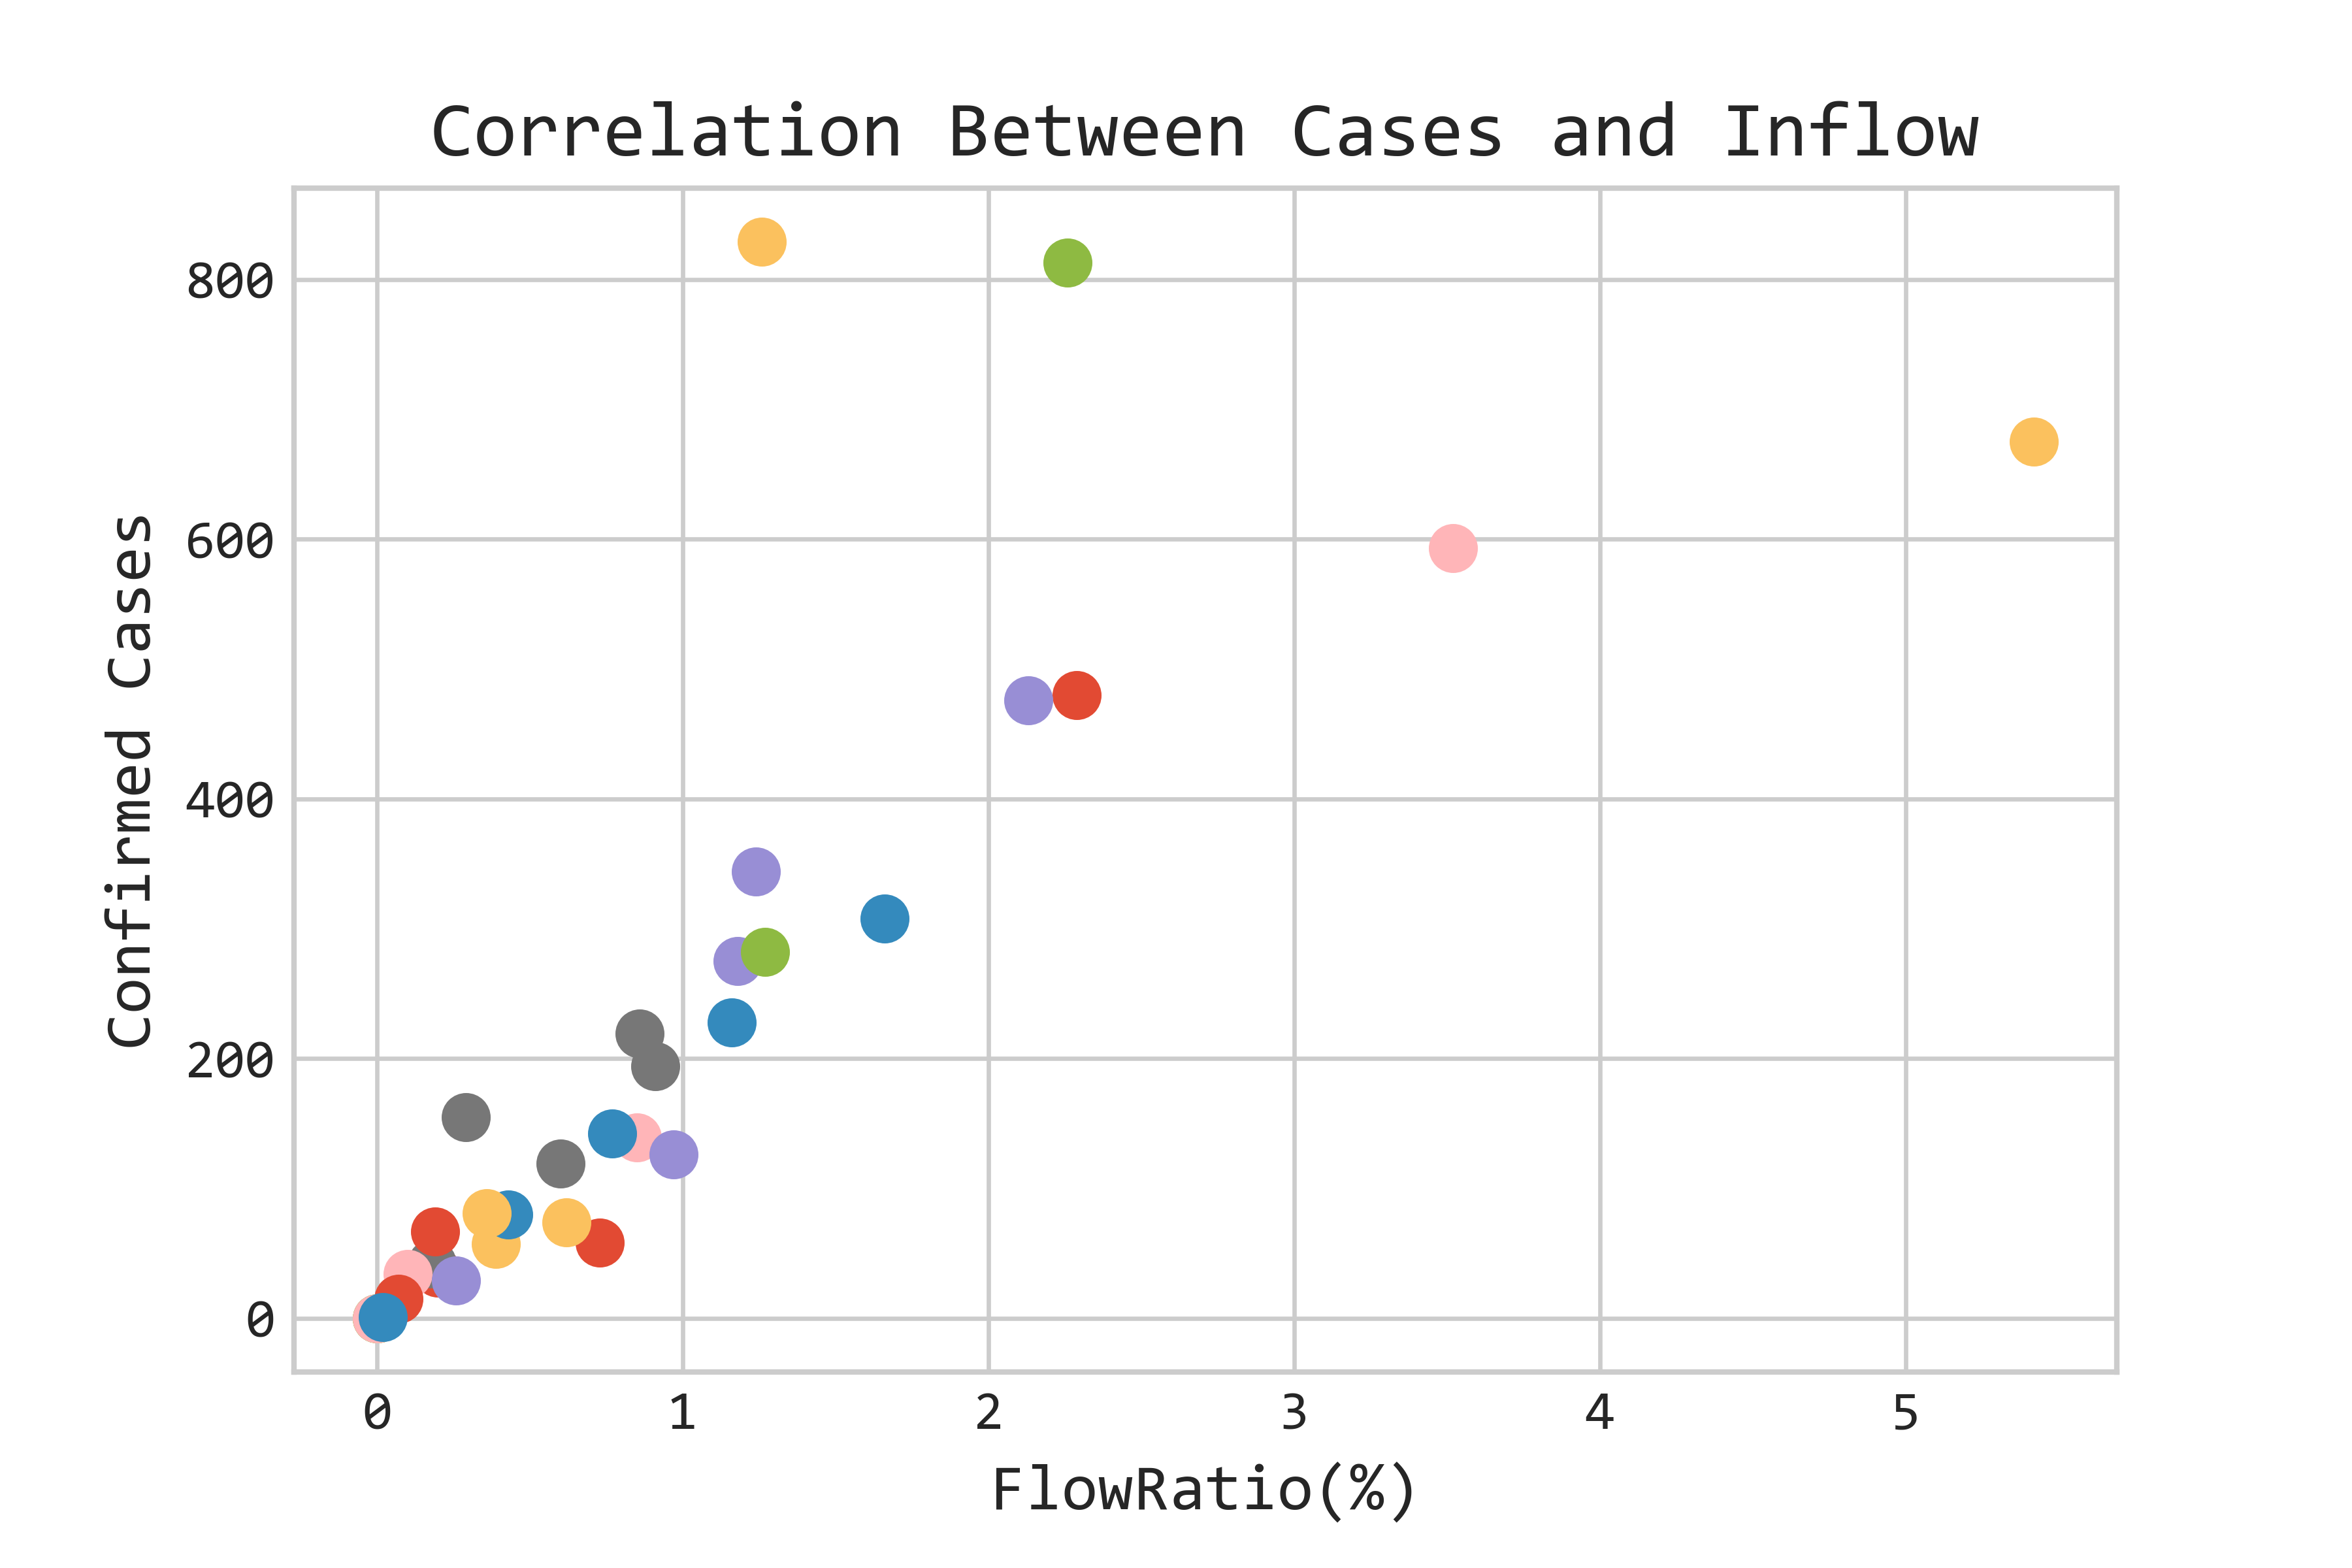
\includegraphics[width=1.0\textwidth]{figure/Relation_Ana.png}
        \caption{Correlation Between Cases and Inflow}
        \label{fig:relation}
    \end{minipage}
\end{figure}

\subsubsection{Iterative Equations} \label{subsubSec:eqn}
Like classic SEIR, first we have $\gamma$ as the chance of getting infected when an uninfected person is close to infectious one, $a$ as the probability of a susceptible individual staying close to an exposed or infectious person, $b$ as the infection efficiency and $h=\gamma a b I$, where $h$ stands for the mathematical expectation of daily infection ratio among $P$. The exposed transitions to infectious at a rate of $\theta$. The total infectious individuals die at a proportion of $k$ and recover at a proportion of $r$ per day.

As we mentioned before, incubation period is a random variable with exponential distribution with parameter $\theta$. We also assume the birth rate equals death rate and thus the total population stays constant. Therefore, the basic form of our model's differential equations can be easily inferred as~\eqref{eqn:cont_diff} $\sim$ (5), where $j \in \lbrace 0, 1, 2 \rbrace$:
\begin{align} \label{eqn:cont_diff}
S_t^{(j)} &= P_t^{(j)} - E_t^{(j)} - I_t^{(j)} - R_t^{(j)} - D_t^{(j)} \\
\frac{{\rm d}E_t^{(j)}}{{\rm d}t} &= hS_t^{(j)} + \left(f_{t, i}^{(j)} - f_{t, o}^{(j)} - \theta\right)E_t^{(j)} \\
\frac{{\rm d}I_t^{(j)}}{{\rm d}t} &= \theta E_t^{(j)} - \left(r + k + f_{t,o}^{(j)} - f_{t,i}^{(j)}\right)I_t^{(j)} \\
\frac{{\rm d}R_t^{(j)}}{{\rm d}t} &= rI_t^{(j)} \\
\frac{{\rm d}D_t^{(j)}}{{\rm d}t} &= kI_t^{(j)}
\end{align}

Considering that the number of a certain group varies little every 24 hours, we use difference equations~\eqref{eqn:disc_diff} $\sim$ (10) instead and iterate once a day in our implementation corresponding to computational efficiency.
\begin{align} \label{eqn:disc_diff}
S_t^{(j)} &= P_t^{(j)} - E_t^{(j)} - I_t^{(j)} - R_t^{(j)} - D_t^{(j)} \\
\Delta E_t^{(j)} &= E_{t+1}^{(j)} - E_t^{(j)} = hS_t^{(j)} + \left(f_{t,i}^{(j)} - f_{t,o}^{(j)} - \theta\right)E_t^{(j)} \\
\Delta I_t^{(j)} &= I_{t+1}^{(j)} - I_t^{(j)} = \theta E_t^{(j)} - \left(r + k + f_{t,o}^{(j)} - f_{t,i}^{(j)}\right)I_t^{(j)} \\
\Delta R_t^{(j)} &= R_{t+1}^{(j)} - R_t^{(j)} = rI_t^{(j)} \\
\Delta D_t^{(j)} &= D_{t+1}^{(j)} - D_t^{(j)} = kI_t^{(j)}
\end{align}

According to our first two assumptions, we have three cases for different regions:
\begin{enumerate}
    \item \textbf{Wuhan} There are little population flow into Wuhan city, meaning we can set $f_{t,i}^{(0)} = 0$ and thus simplify our difference equations (7) and (8) as following:
    \begin{align}
        \Delta E_t^{(0)} &= E_{t+1}^{(0)} - E_t^{(0)} = hS_t^{(0)} - \left(f_{t,o}^{(0)} + \theta\right)E_t^{(0)} \\
        \Delta I_t^{(0)} &= I_{t+1}^{(0)} - I_t^{(0)} = \theta E_t^{(0)} - \left(r + k + f_{t,o}^{(0)}\right)I_t^{(0)}
    \end{align}
    \item \textbf{Hubei except for Wuhan} A large proportion (up to two thirds) of Wuhan's outflow population does not leave Hubei province, causing the epidemic situation in other regions inside Hubei deeply influenced by this group. Simultaneously, we can reasonably leave out the outflow in this case as the density of virus carriers is much lower. So just let $f_{t,o}^{(0)} = 0$ in equations (7) and (8), and we will obtain the simplified equations specifically:
    \begin{align}
        \Delta E_t^{(1)} &= E_{t+1}^{(1)} - E_t^{(1)} = hS_t^{(1)} + \left(f_{t,i}^{(1)} - \theta\right)E_t^{(1)} \\
        \Delta I_t^{(1)} &= I_{t+1}^{(1)} - I_t^{(1)} = \theta E_t^{(1)} - \left(r + k - f_{t,i}^{(1)}\right)I_t^{(1)}
    \end{align}
    When considering the whole Hubei Province, we add the two cases above together.
    \item \textbf{Other Provinces} As virus carrier flows from these regions are ignored, we still have $f_{t,o}^{(2)} = 0$ and thus get the simplified expressions for $\Delta E_t$ and $\Delta I_t$ the same as equations (13) and (14).
\end{enumerate}

\subsubsection{Parameter Determination} \label{subSec:Para}
In our modified SEIR model, we need to choose suitable values for five parameters, which is $\theta$, $r$, $k$, $\gamma$, and $b$. As will be shown in Section~\ref{Sec:analysis}, some of them tend to have visible impacts on our model’s performance.

\begin{itemize}
    \item Some researchers have given their predictions of 2019-nCoV's incubation period, ranging from five to eight days, as mentioned in~\cite{inc_1,inc_2, inc_3}. Without loss of generality, we take one week as the incubation period, and thus $\theta = 1 / 7$.
    \item The average mortality and survival rate has leveled off in the past few days, and we take $3.5\%$ for both of them. And we assume a one-week recover period $\lambda^{-1} = 7$ for each 'infectious' on average. Based on the theory of exponential distribution, we have $k = 0.035\lambda = 0.5\%$ all the time, $r = 0.035\lambda = 0.5\%$ in the first 30 days and $r = 2 \times 0.035\lambda = 1.0\%$ as the more infected people are diagnosed and treated earlier.
    \item According to recent news, the spread ability of 2019-nCoV is astonishing, as a large proportion of the infectious got infected during a very short stay with other carriers. Thus we choose a large constant, letting $\gamma = 0.75$.
    \item Till now there have not been many works focusing on the infection efficiency of the virus, and from collected information we only infer that its $b$ is no less than that of SARS in 2003. Therefore, we use $b = 0.6$, same as the value often used for SARS.
\end{itemize}

\subsubsection{Basic Reproductive Number} \label{subsubSec:R0}
Here we introduce the concept of basic reproductive number $R_0$, which an important concept in the evaluation of infectious diseases. In SEIR model without dynamic birth and death, $R_0$ is defined by Equation~\eqref{eqn:classic_R0}:
\begin{equation} \label{eqn:classic_R0}
    R_0 = \frac{\gamma a b P}{\lambda}
\end{equation}
Where $\gamma$, $a$, $b$, $P$, and $\lambda$ have the same definitions as in this article.

Based on the parameters of our model, we can compute $R_0$ of 2019-nCoV as following:
\begin{equation*}
    R_0 = \frac{0.75 \times 0.6 \times P}{1 / 7 \times P} = 3.15
\end{equation*}
Which is generally consistent with the given values in other works.

The basic reproductive number $R_0$ is the initial mathematical expectation of infections brought by a single infected individual, which measures the spread ability of virus. As time goes by, the reproductive number $R_0$ might have different values, and the sufficient and necessary condition for continuous spread of an infectious disease is that it has its $R_0 \geq 1$. If $R_0 \textless 1$, the virus become extinct eventually. The $R_0$ of SARS is estimated in the range 2 to 4, but this virus is more contagious and we have better medical conditions, too. Above all, we think our $3.15$ would be a reasonable estimate.

\subsection{Implementation and Result}

\subsubsection{Model Validation}
First we validate our modified SEIR model on some provinces' statistics. However, we find that the predictions are not exactly consistent with in some provinces, which is reasonably caused by the inaccuracy of population flow proportion between provinces. The uncertainty in the spread process of the disease should also be taken into consideration. For example, one infected person may influence all in his/her carriage and the ratio may deviate from the collected data. Therefore, we modify the population flow into specific provinces in order to make more precise predictions. 

\begin{figure}[htbp]
    \centering
    \begin{subfigure}[t]{0.45\textwidth}
        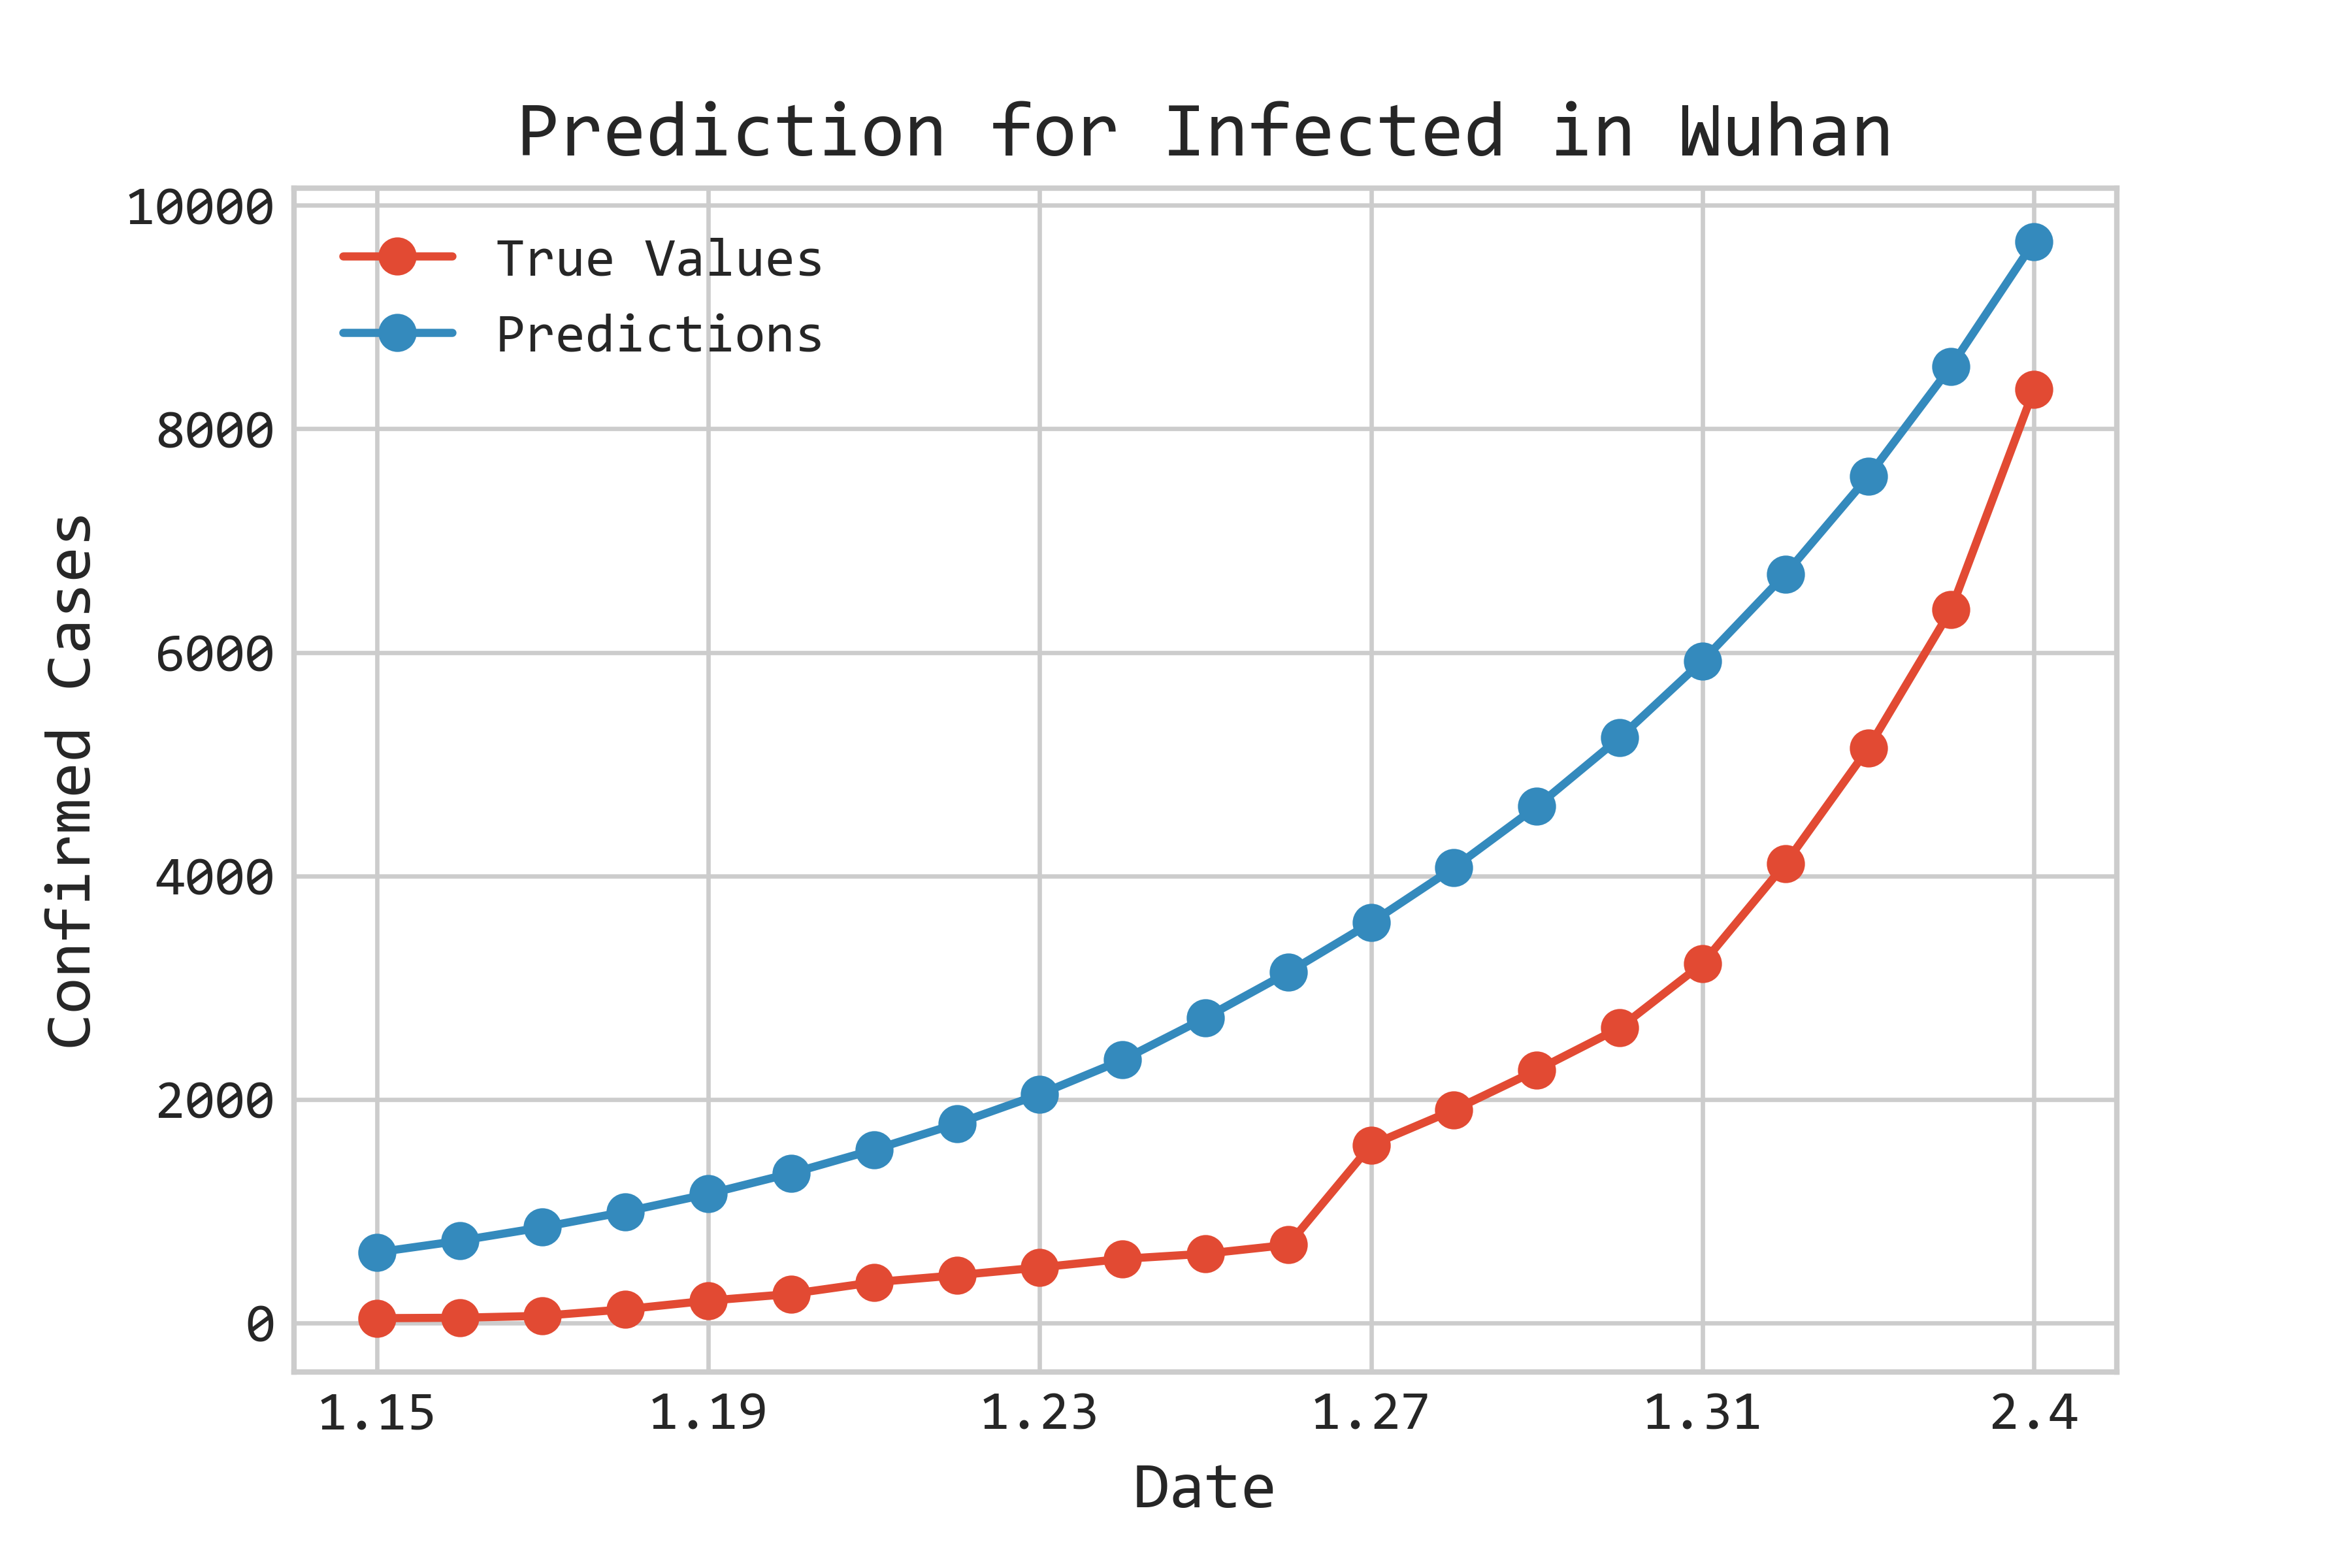
\includegraphics[width=1.0\textwidth]{figure/Wuhan_Comp.png}
        \caption{Wuhan}
        \label{fig:Val_Wuhan}
    \end{subfigure}
    \begin{subfigure}[t]{0.45\textwidth}
        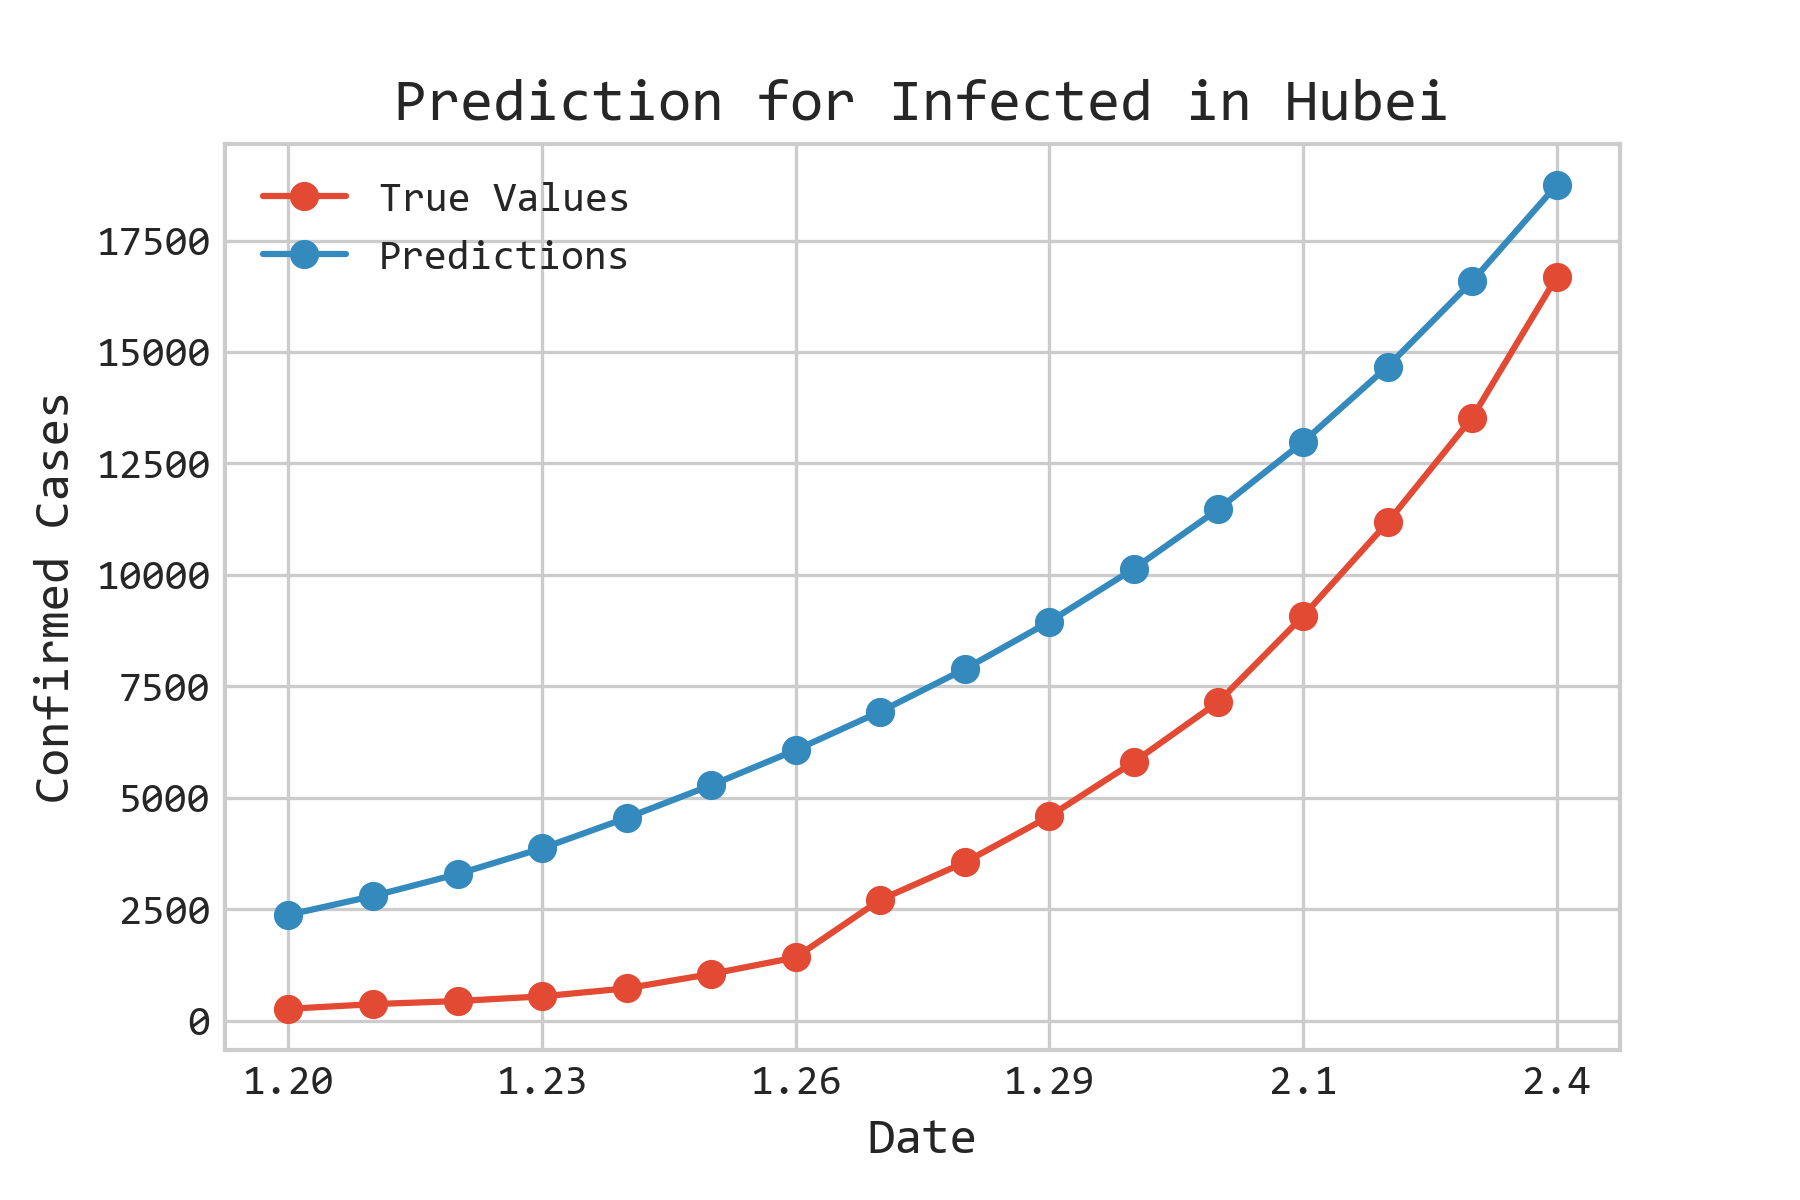
\includegraphics[width=1.0\textwidth]{figure/Hubei_Comp.png}
        \caption{Hubei}
        \label{fig:Val_Hubei}
    \end{subfigure}
    \\
    \begin{subfigure}[t]{0.45\textwidth}
        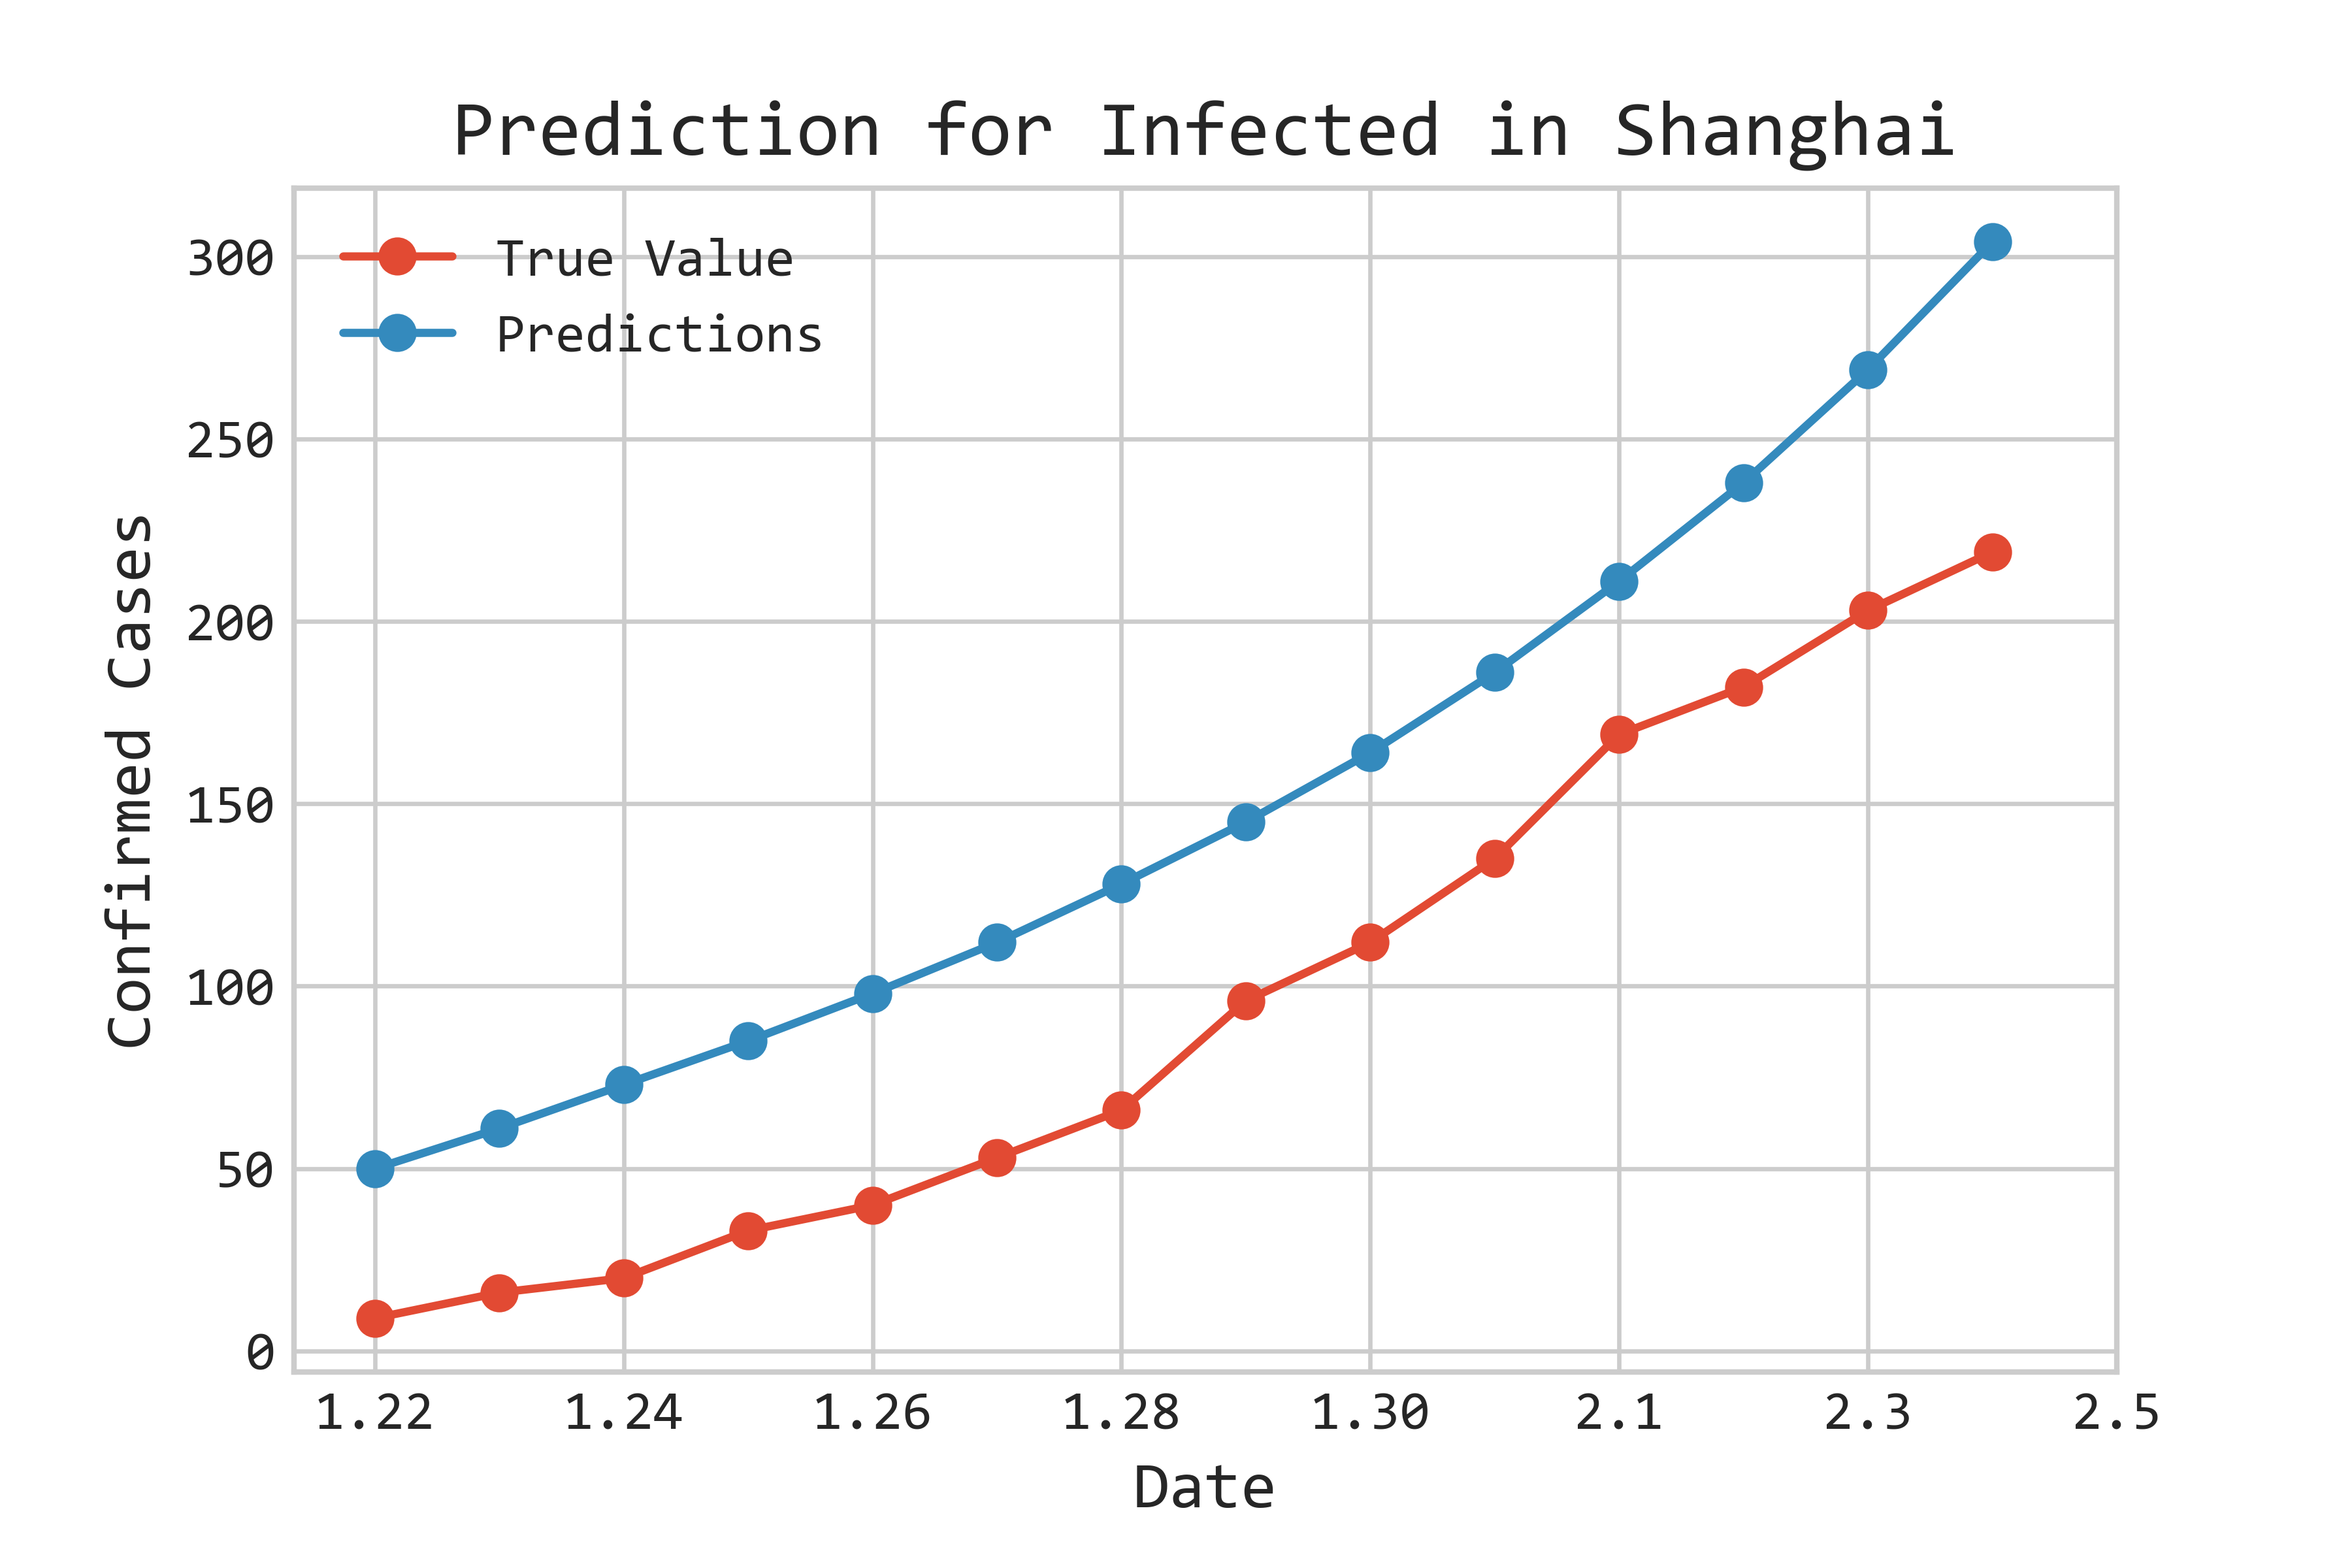
\includegraphics[width=1.0\textwidth]{figure/Shanghai_Validation.png}
        \caption{Shanghai}
        \label{fig:Val_Shanghai}
    \end{subfigure}
    \begin{subfigure}[t]{0.45\textwidth}
        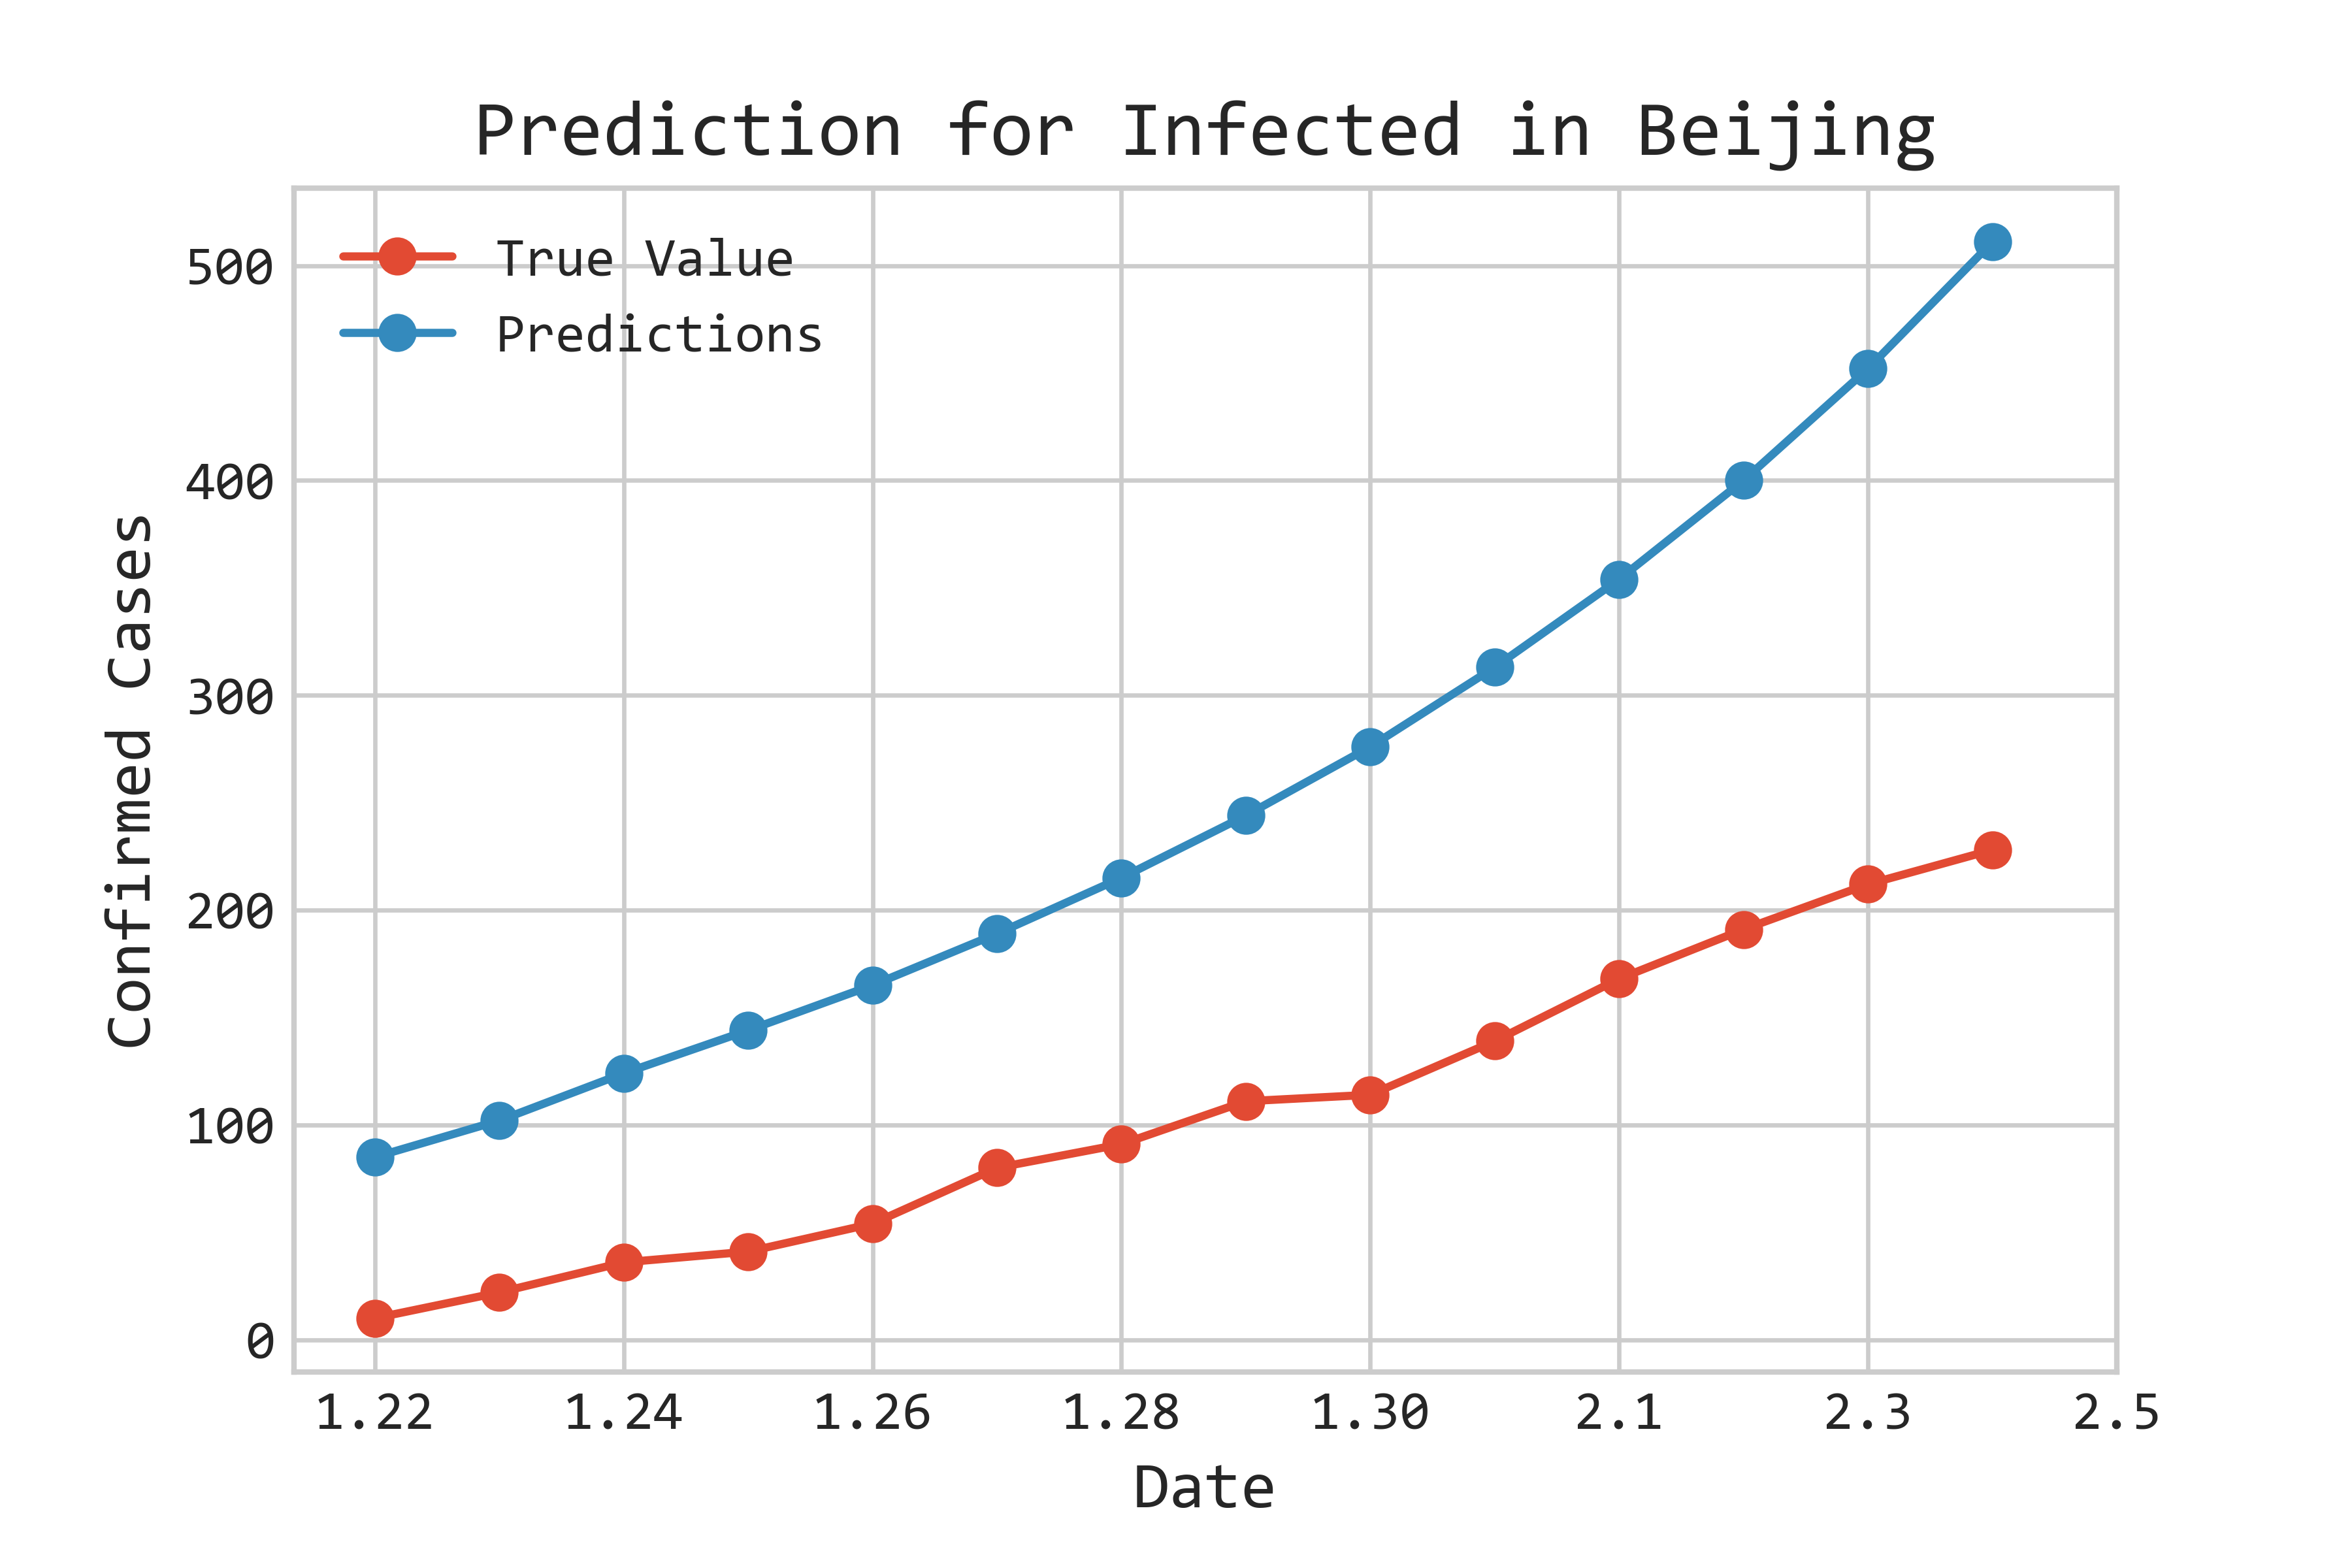
\includegraphics[width=1.0\textwidth]{figure/Beijing_Validation.png}
        \caption{Beijing}
        \label{fig:Val_Beijing}
    \end{subfigure}
    \caption{Model Validation on the Datasets of Some Regions}
    \label{fig:Val}
\end{figure}

 Predictions for Wuhan and several provinces are shown in Figure~\ref{fig:Val}. We point out that we predict the infected cases in Figure~\ref{fig:Val} and the confirmed case is not equal to the infected case because some infected cases are not confirmed timely. That is to say, it is reasonable that the predicted number is higher that of confirmed cases publicly announced. Therefore, it is justified that our model is highly consistent with reality of last two weeks.

\begin{figure}[hb]
    \centering
    \includegraphics[width=0.9\textwidth]{053/figure/China_Total_Prediction.png}
    \caption{Domestic Infection Prediction}
    \label{fig:domestic}
\end{figure}

\subsubsection{Domestic and Global Predictions} \label{subsec:pred}
With its effectiveness proved, the modified compartmental SEIR now can be used to predict the domestic and global infections in the next period of time.

Considering domestic infections, we divide Chinese mainland into 31 provinces, and then implement our model using corresponding iteration equations on each of them. Finally we take the summation of all provinces' predicted value as our prediction for domestic infections. Our predictions can be seen in Figure~\ref{fig:domestic}.

\begin{figure}[H]
    \captionsetup{font={small}}
    \centering
        \begin{minipage}[c]{0.48\textwidth}
            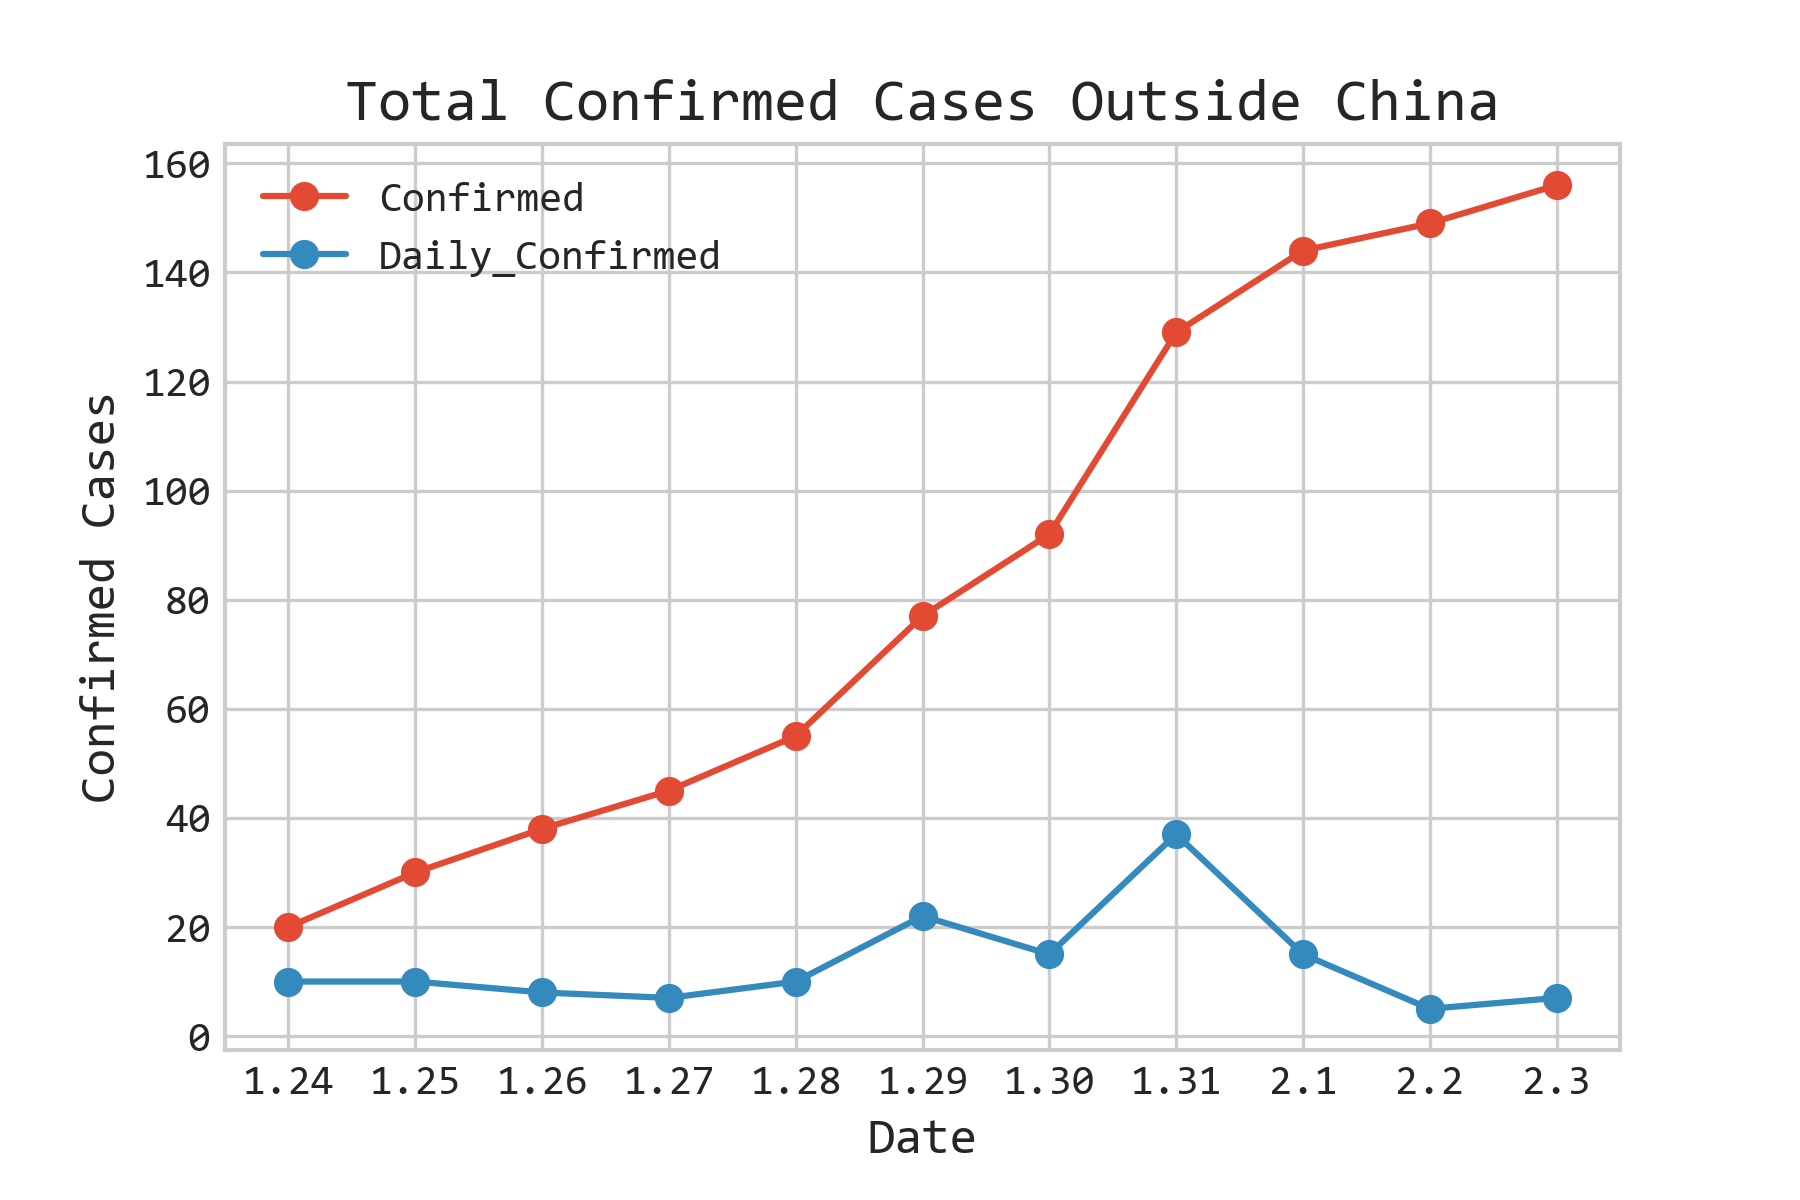
\includegraphics[width=1.0\textwidth]{figure/Global_Total.png}
            \caption{Total Confirmed Cases Outside China}
            \label{fig:Glob_Total}
        \end{minipage}
        \begin{minipage}[c]{0.48\textwidth}
            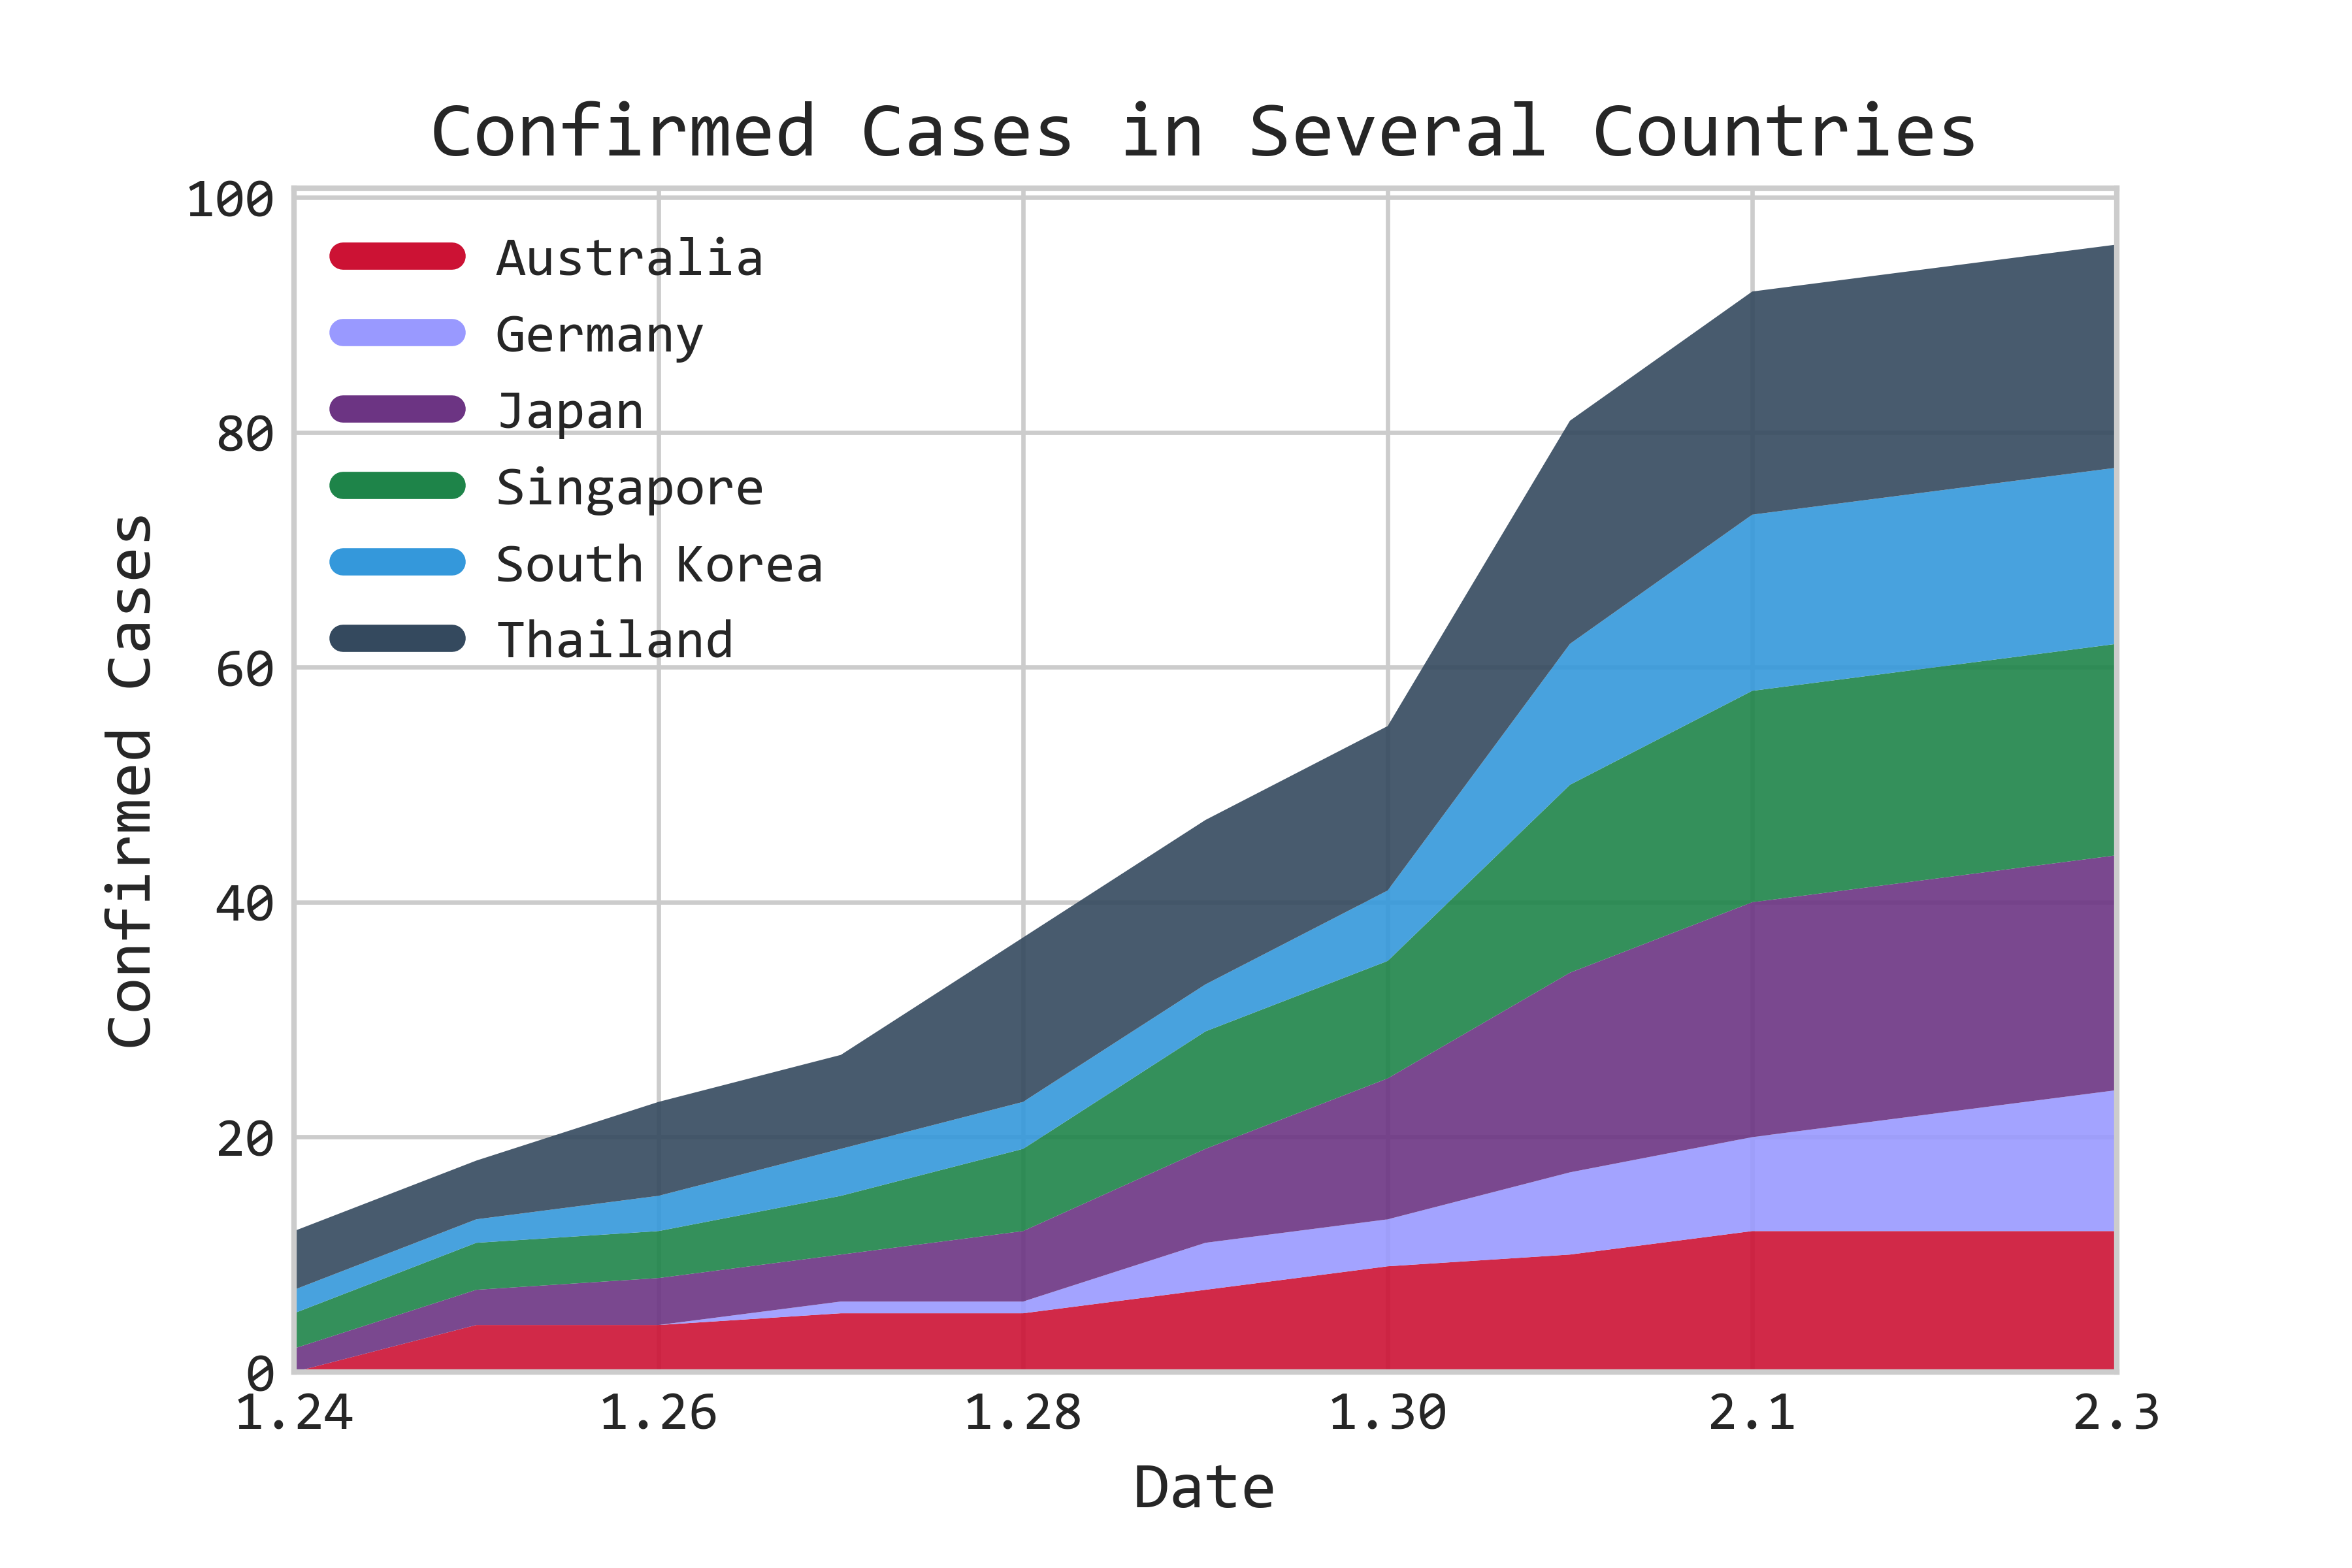
\includegraphics[width=1.0\textwidth]{figure/Global_Partial.png}
            \caption{Confirmed Cases in Some Countries}
            \label{fig:Glob_Partial}
        \end{minipage}
\end{figure}

As for global infections, we first analyze the situation from Jan. 24 to Feb. 3 because the influence of 2019-nCoV came to emerge outside China around Jan. 24.

As is shown in Figure~\ref{fig:Glob_Total}, the total confirmed cases outside China were on a daily increase of less than 40. Figure~\ref{fig:Glob_Partial} indicates confirmed cases in countries suffering relatively seriously from 2019-nCov, mainly attributed to geological reason and  international population flow. Generally speaking, the confirmed cases is under 20 cases in a single country. Therefore, outside China, the outbreak of 2019-nCov is discretely distributed and kept under control.

\begin{figure}[H]
    \centering
    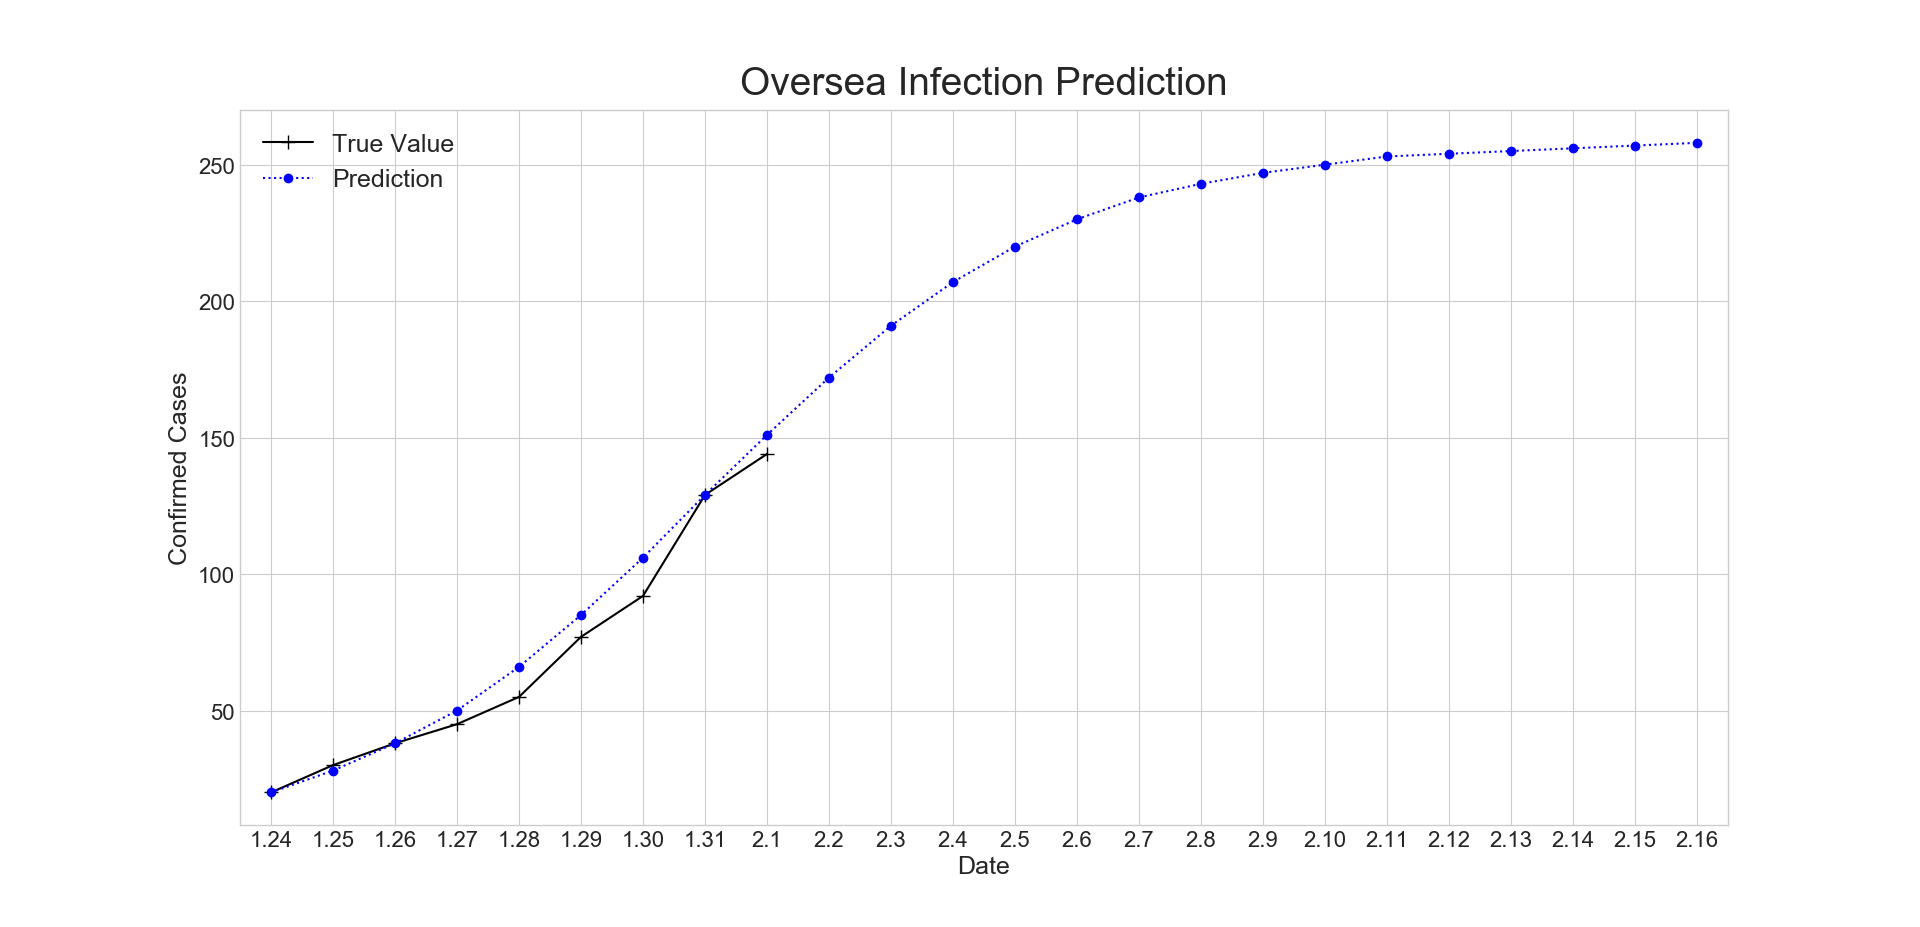
\includegraphics[width=0.9\textwidth]{figure/Oversea_Prediction.png}
    \caption{Oversea Infection Prediction}
    \label{fig:oversea}
\end{figure}

Considering the poor statistics from other countries and the influences brought by potential uncertain factors, we choose the grey prediction model Grey Verhulst to forecast the trend of oversea infections because it can take into account the spread saturability of virus under powerful control, and then obtain the result in Figure~\ref{fig:oversea}, which indicates that the number of oversea infections is about to level off in the next two weeks and the main reasons might be early discovery, timely isolation and travel restriction from China.

\begin{figure}[H]
    \centering
    \begin{subfigure}[b]{0.48\textwidth}
        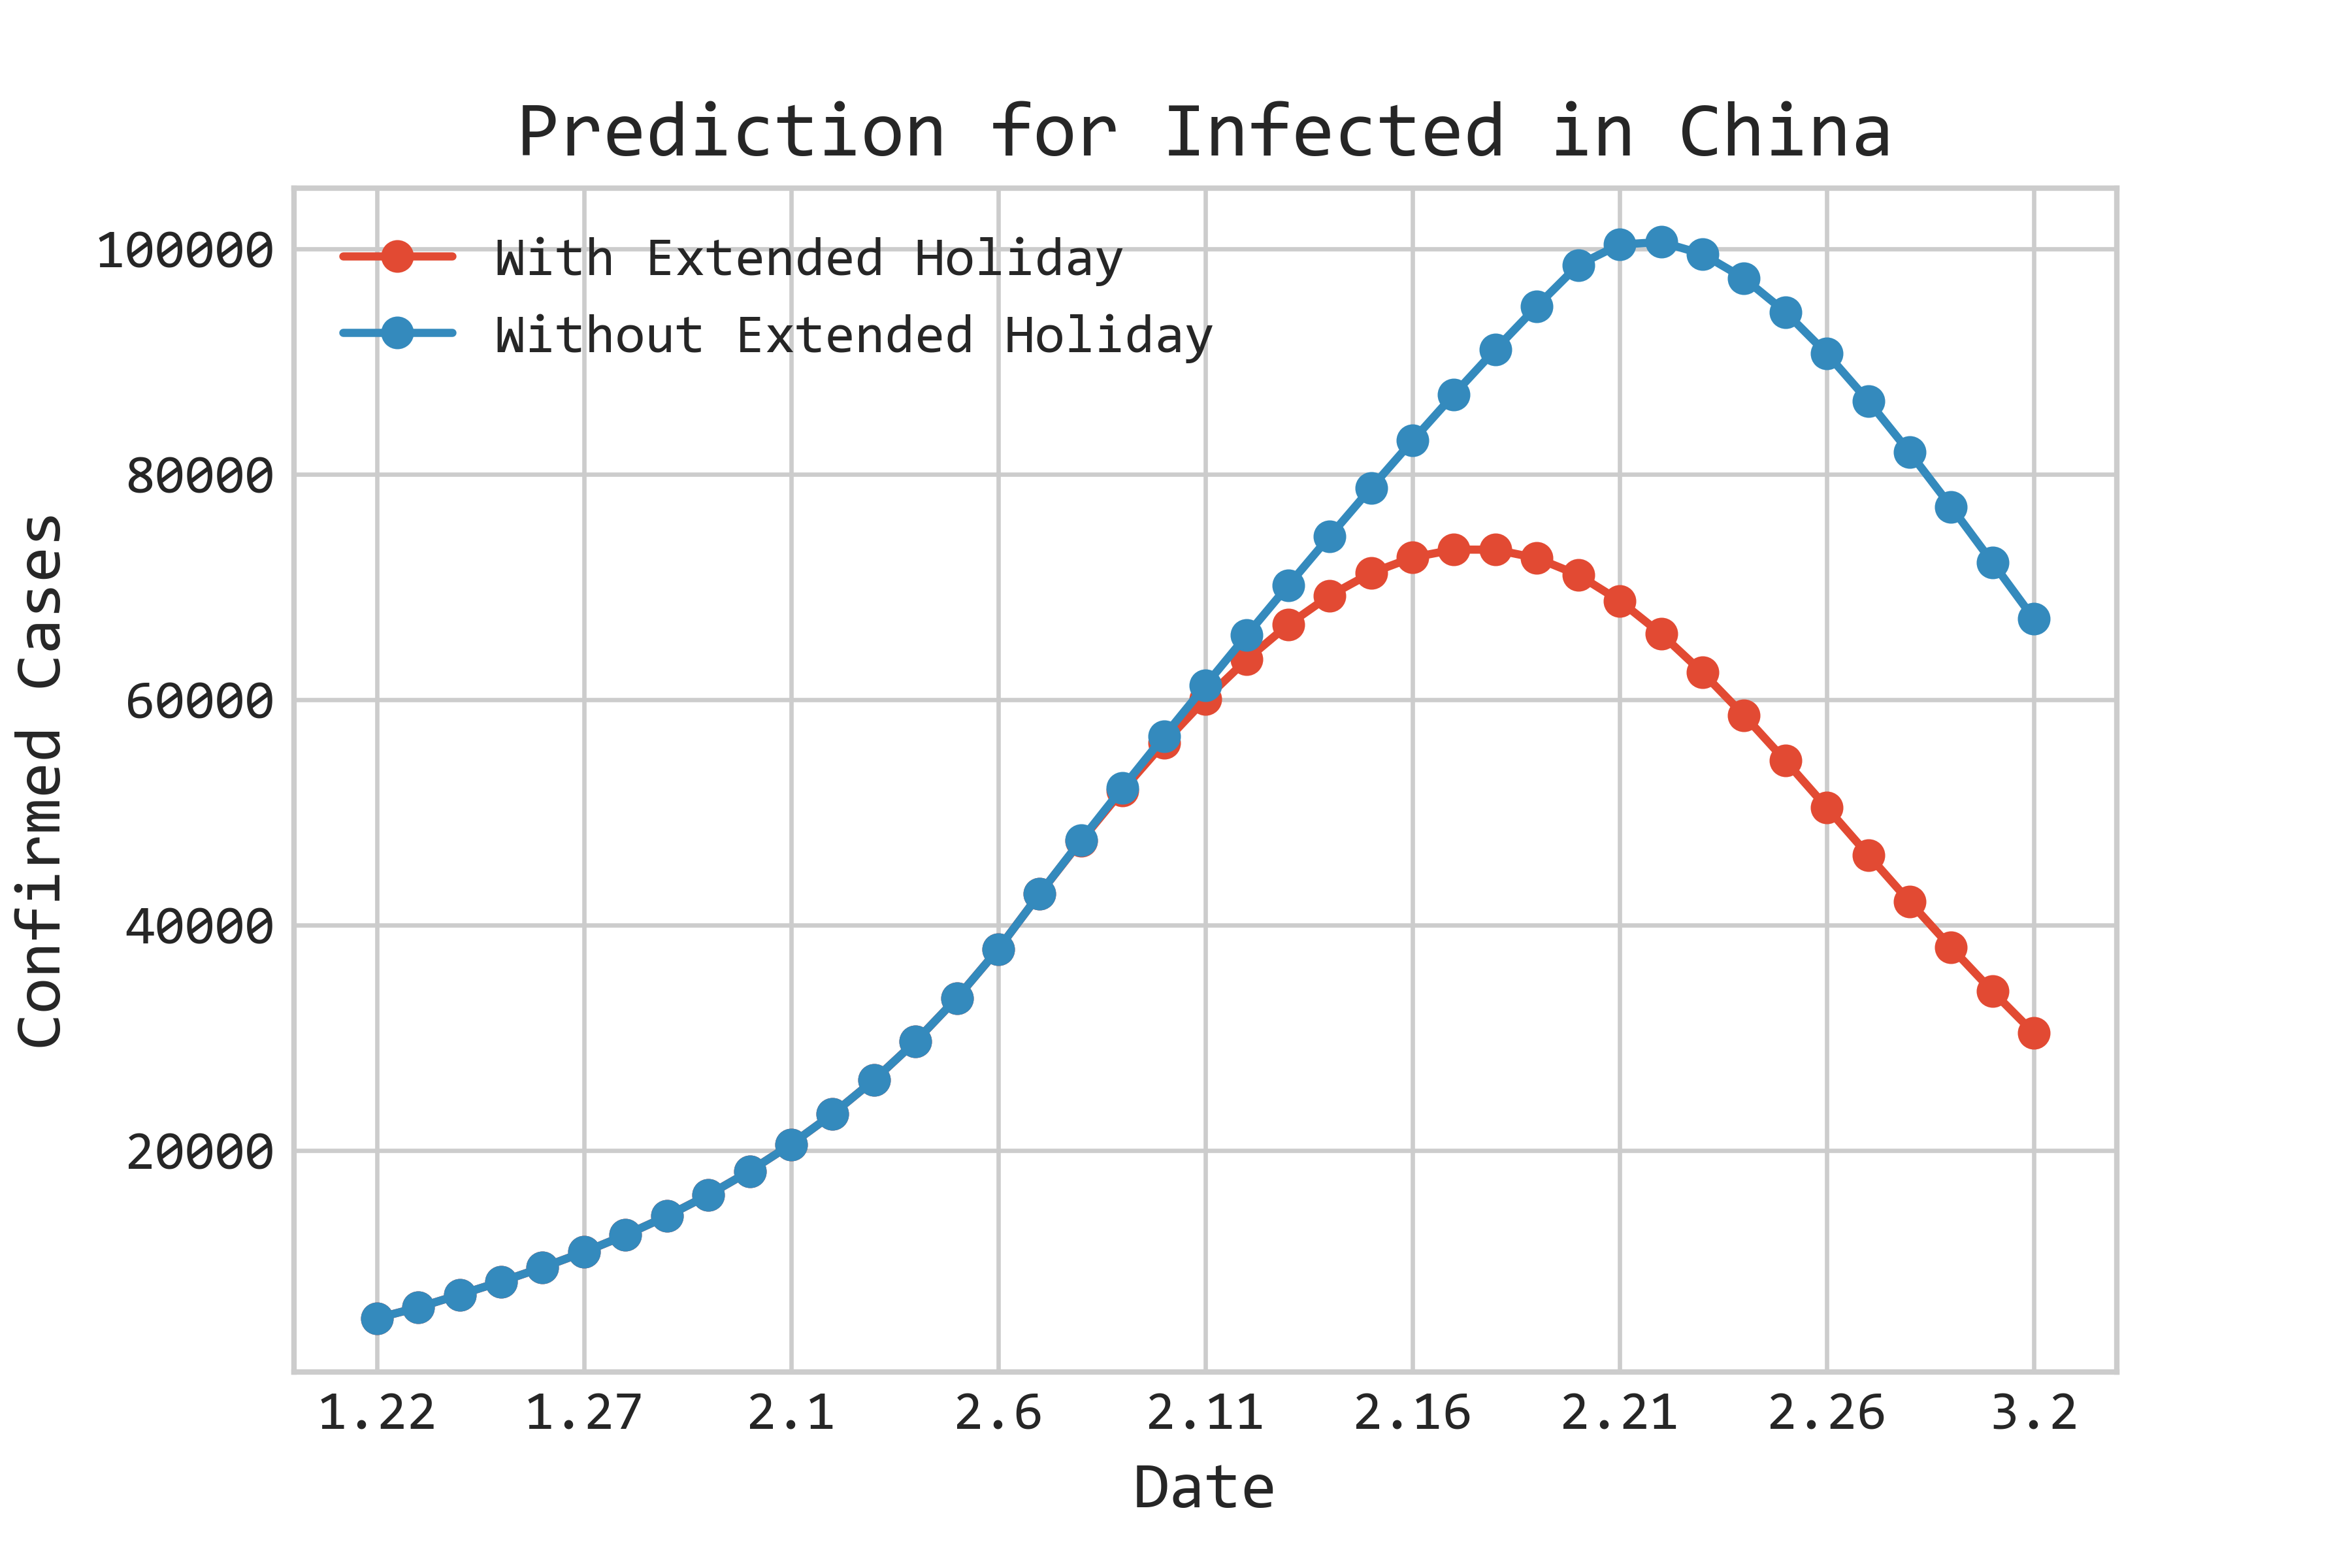
\includegraphics[width=\textwidth]{figure/China_Total_Holiday_Comp.png}
        \caption{\small{Holiday Extension}}
        \label{fig:Holidaay}
    \end{subfigure}%
    \begin{subfigure}[b]{0.48\textwidth}
        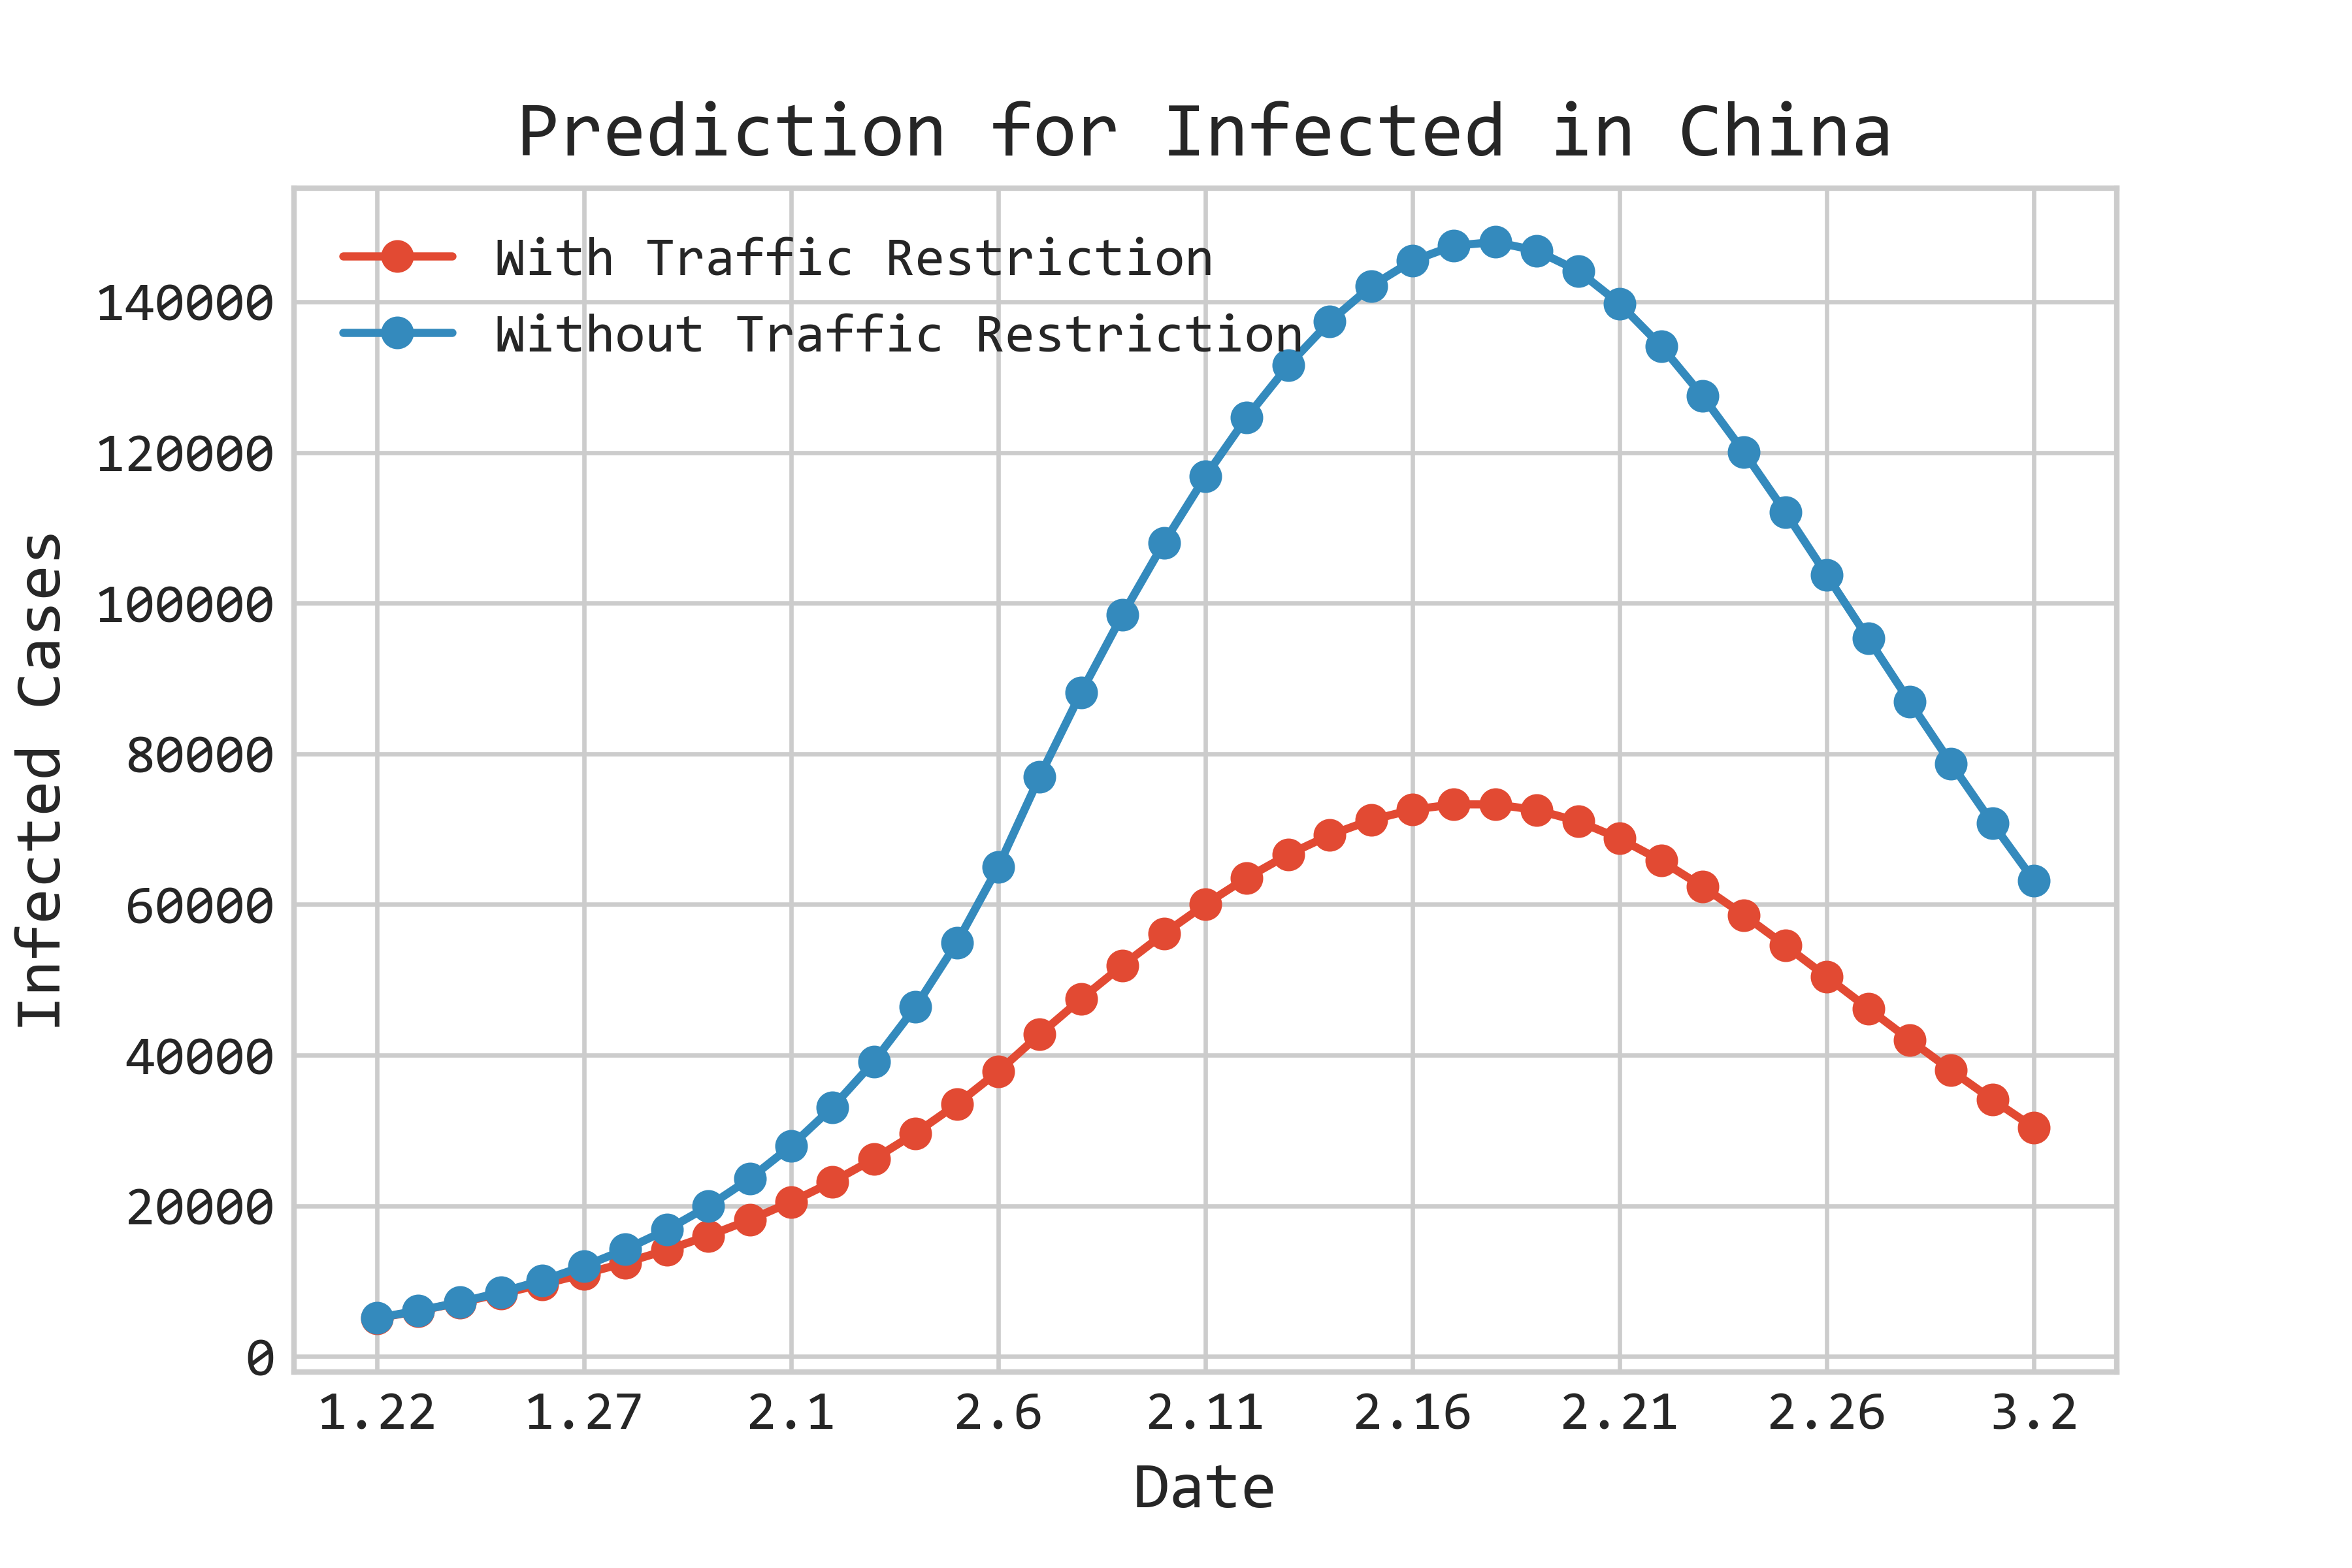
\includegraphics[width=\textwidth]{figure/Prediction_Without_Traf_Rest.png}
        \caption{\small{Traffic Restriction}}
        \label{fig:Traf_Rest}
    \end{subfigure}
    \caption{Quantification of Measures' effect}\label{fig:Measures}
\end{figure}

\subsubsection{Quantification of Measures' Effect}
    We have presented our model's prediction in Section~\ref{subsec:pred} with major control measures taken by the Chinese government, including travel restriction and holiday extension. To analyze the effectiveness of these measures, in this part we will exhibit our predictions without the influence of them as comparison.
    
    As illustrated in Figure ~\ref{fig:Stack_No_Tra_Rest}, policies like quarantine, travel limitations and holiday extension do blunt the outbreak's impacts. Up to 68\% potential infections have been cut according to our speculation. To be more specific, travel limitations arrest the soaring infections during traditional Chinese new year and the extended holiday put off the massive influx of people in the city which could get the outbreak out of control. Some other measures like temperature check stations and suspension of public transportation play their parts too. But for all these prompt measures, the virus could have claimed far longer lives.

\begin{figure}[H]
    \centering
    \begin{subfigure}[b]{0.3\textwidth}
        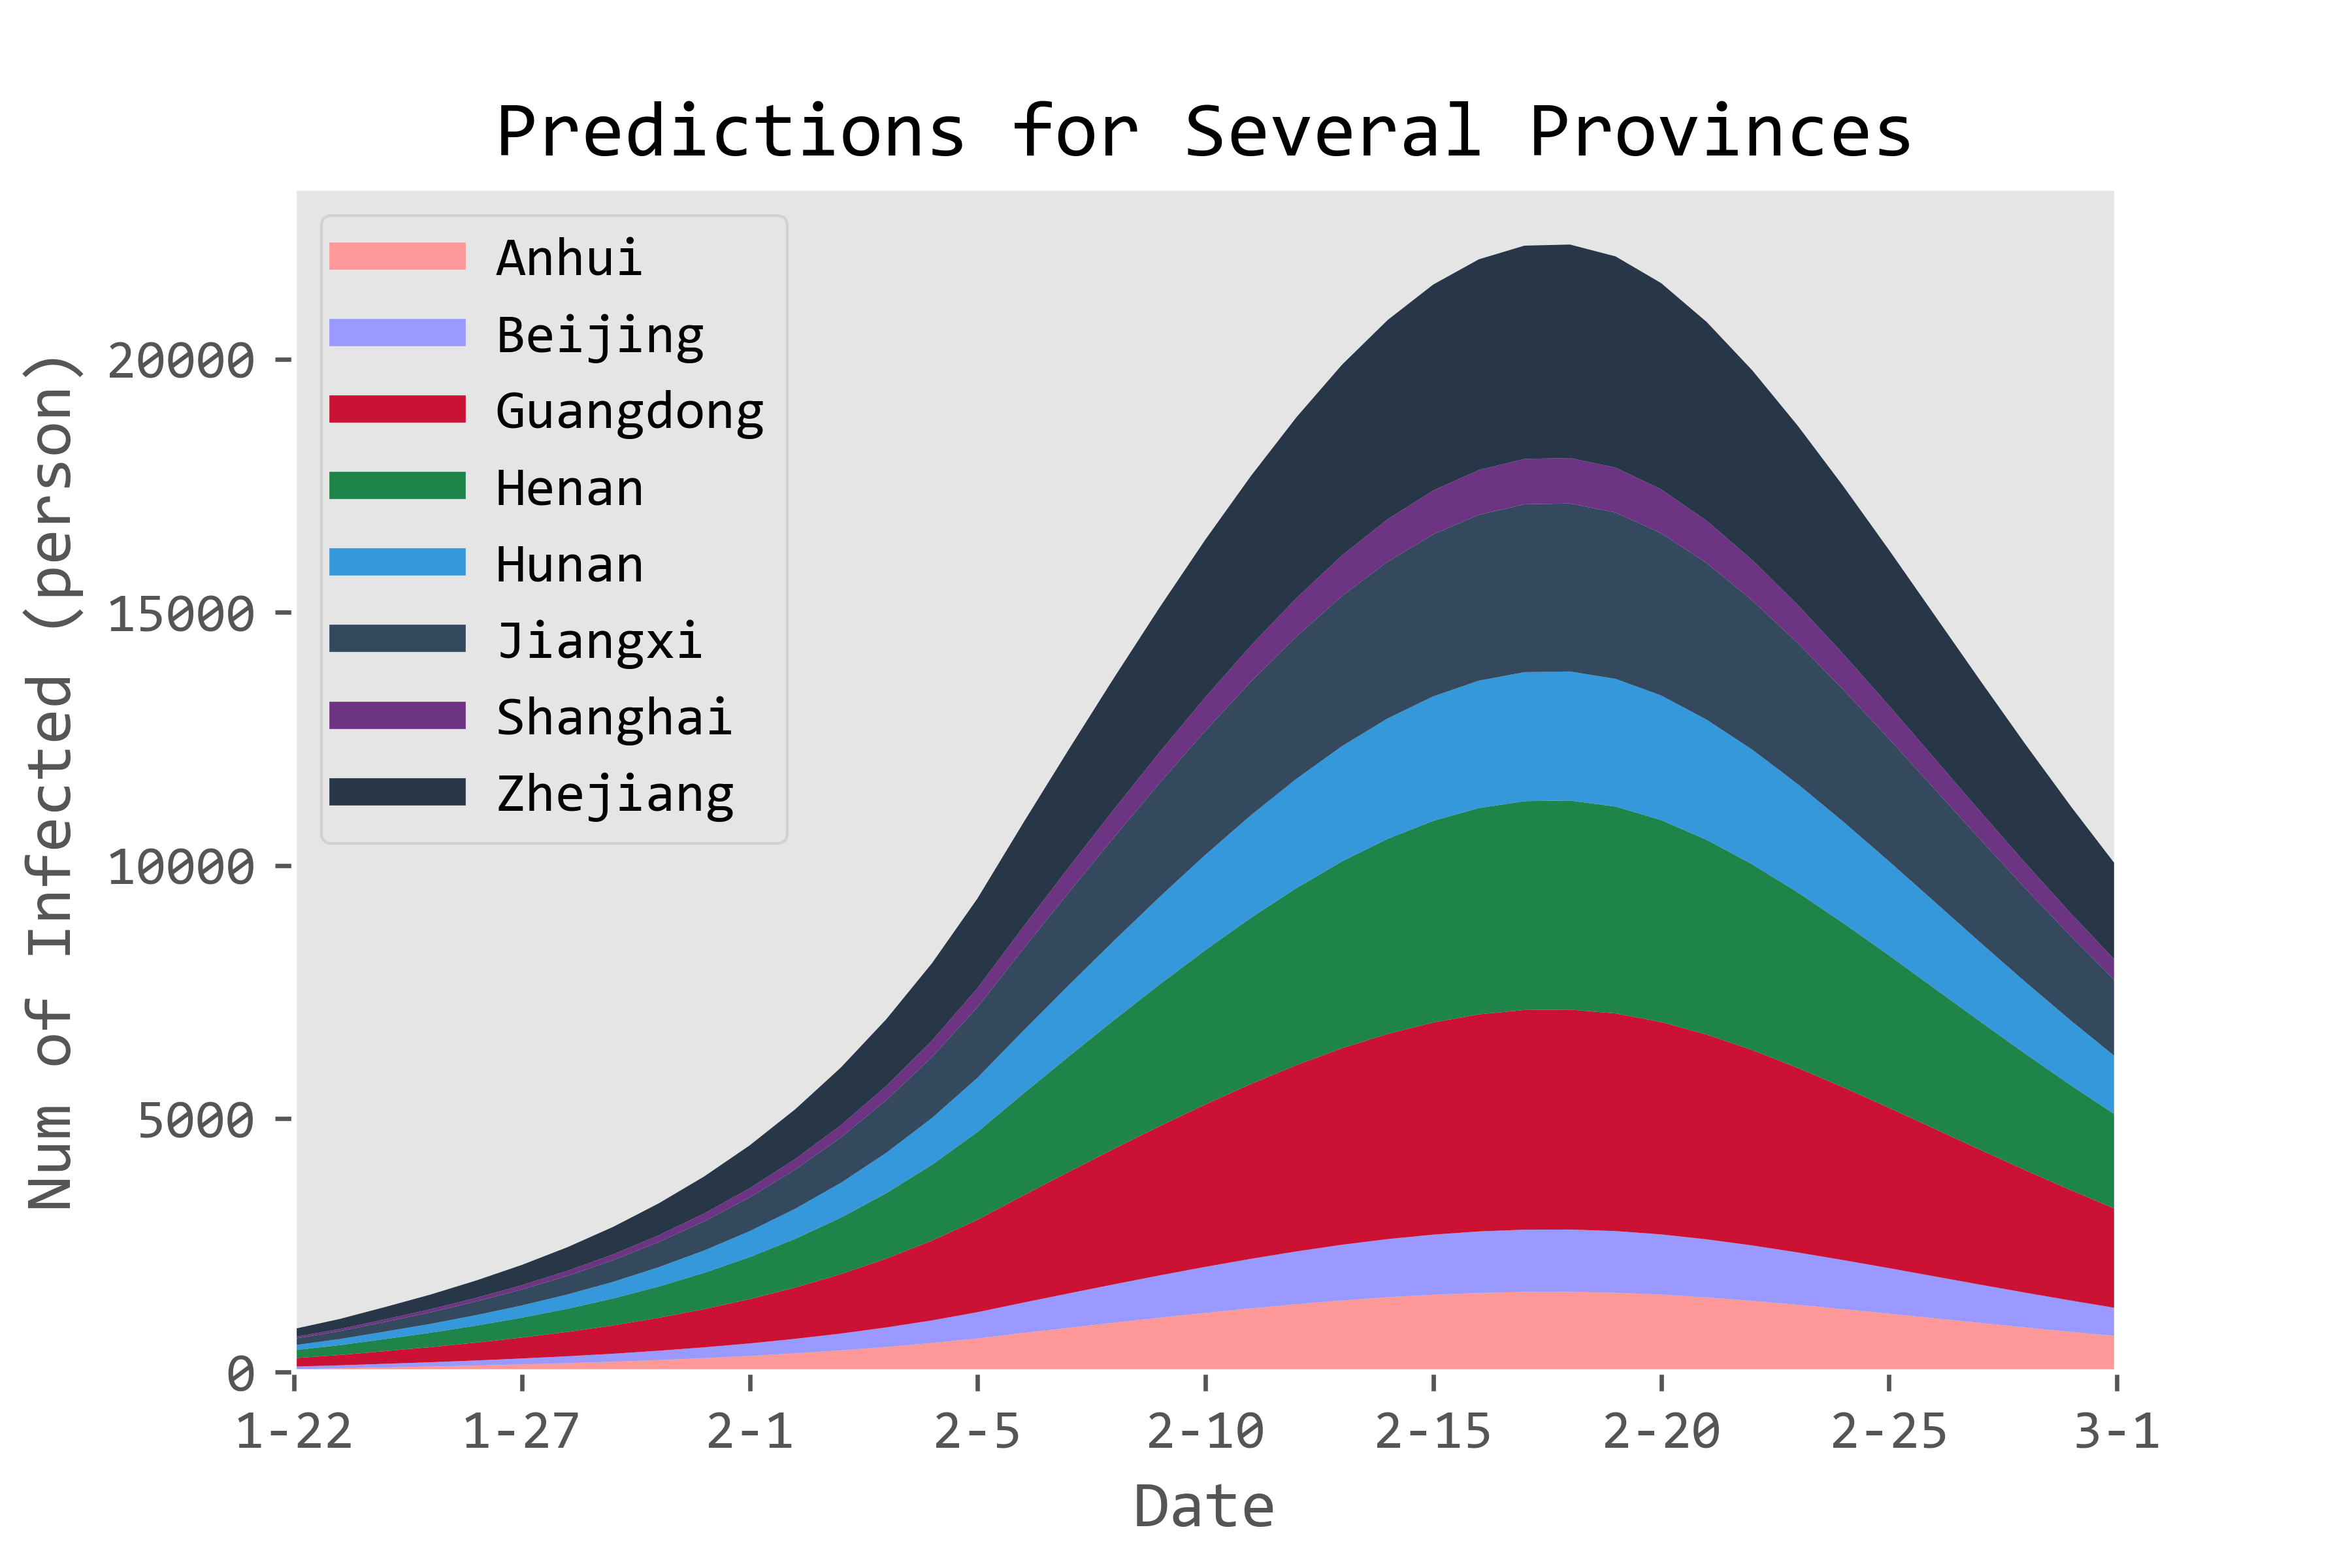
\includegraphics[width=\textwidth]{figure/Stack_Province.png}
        \caption{\small{Effective Measures}}
        \label{fig:Stack_Both}
    \end{subfigure}%
    \begin{subfigure}[b]{0.3\textwidth}
        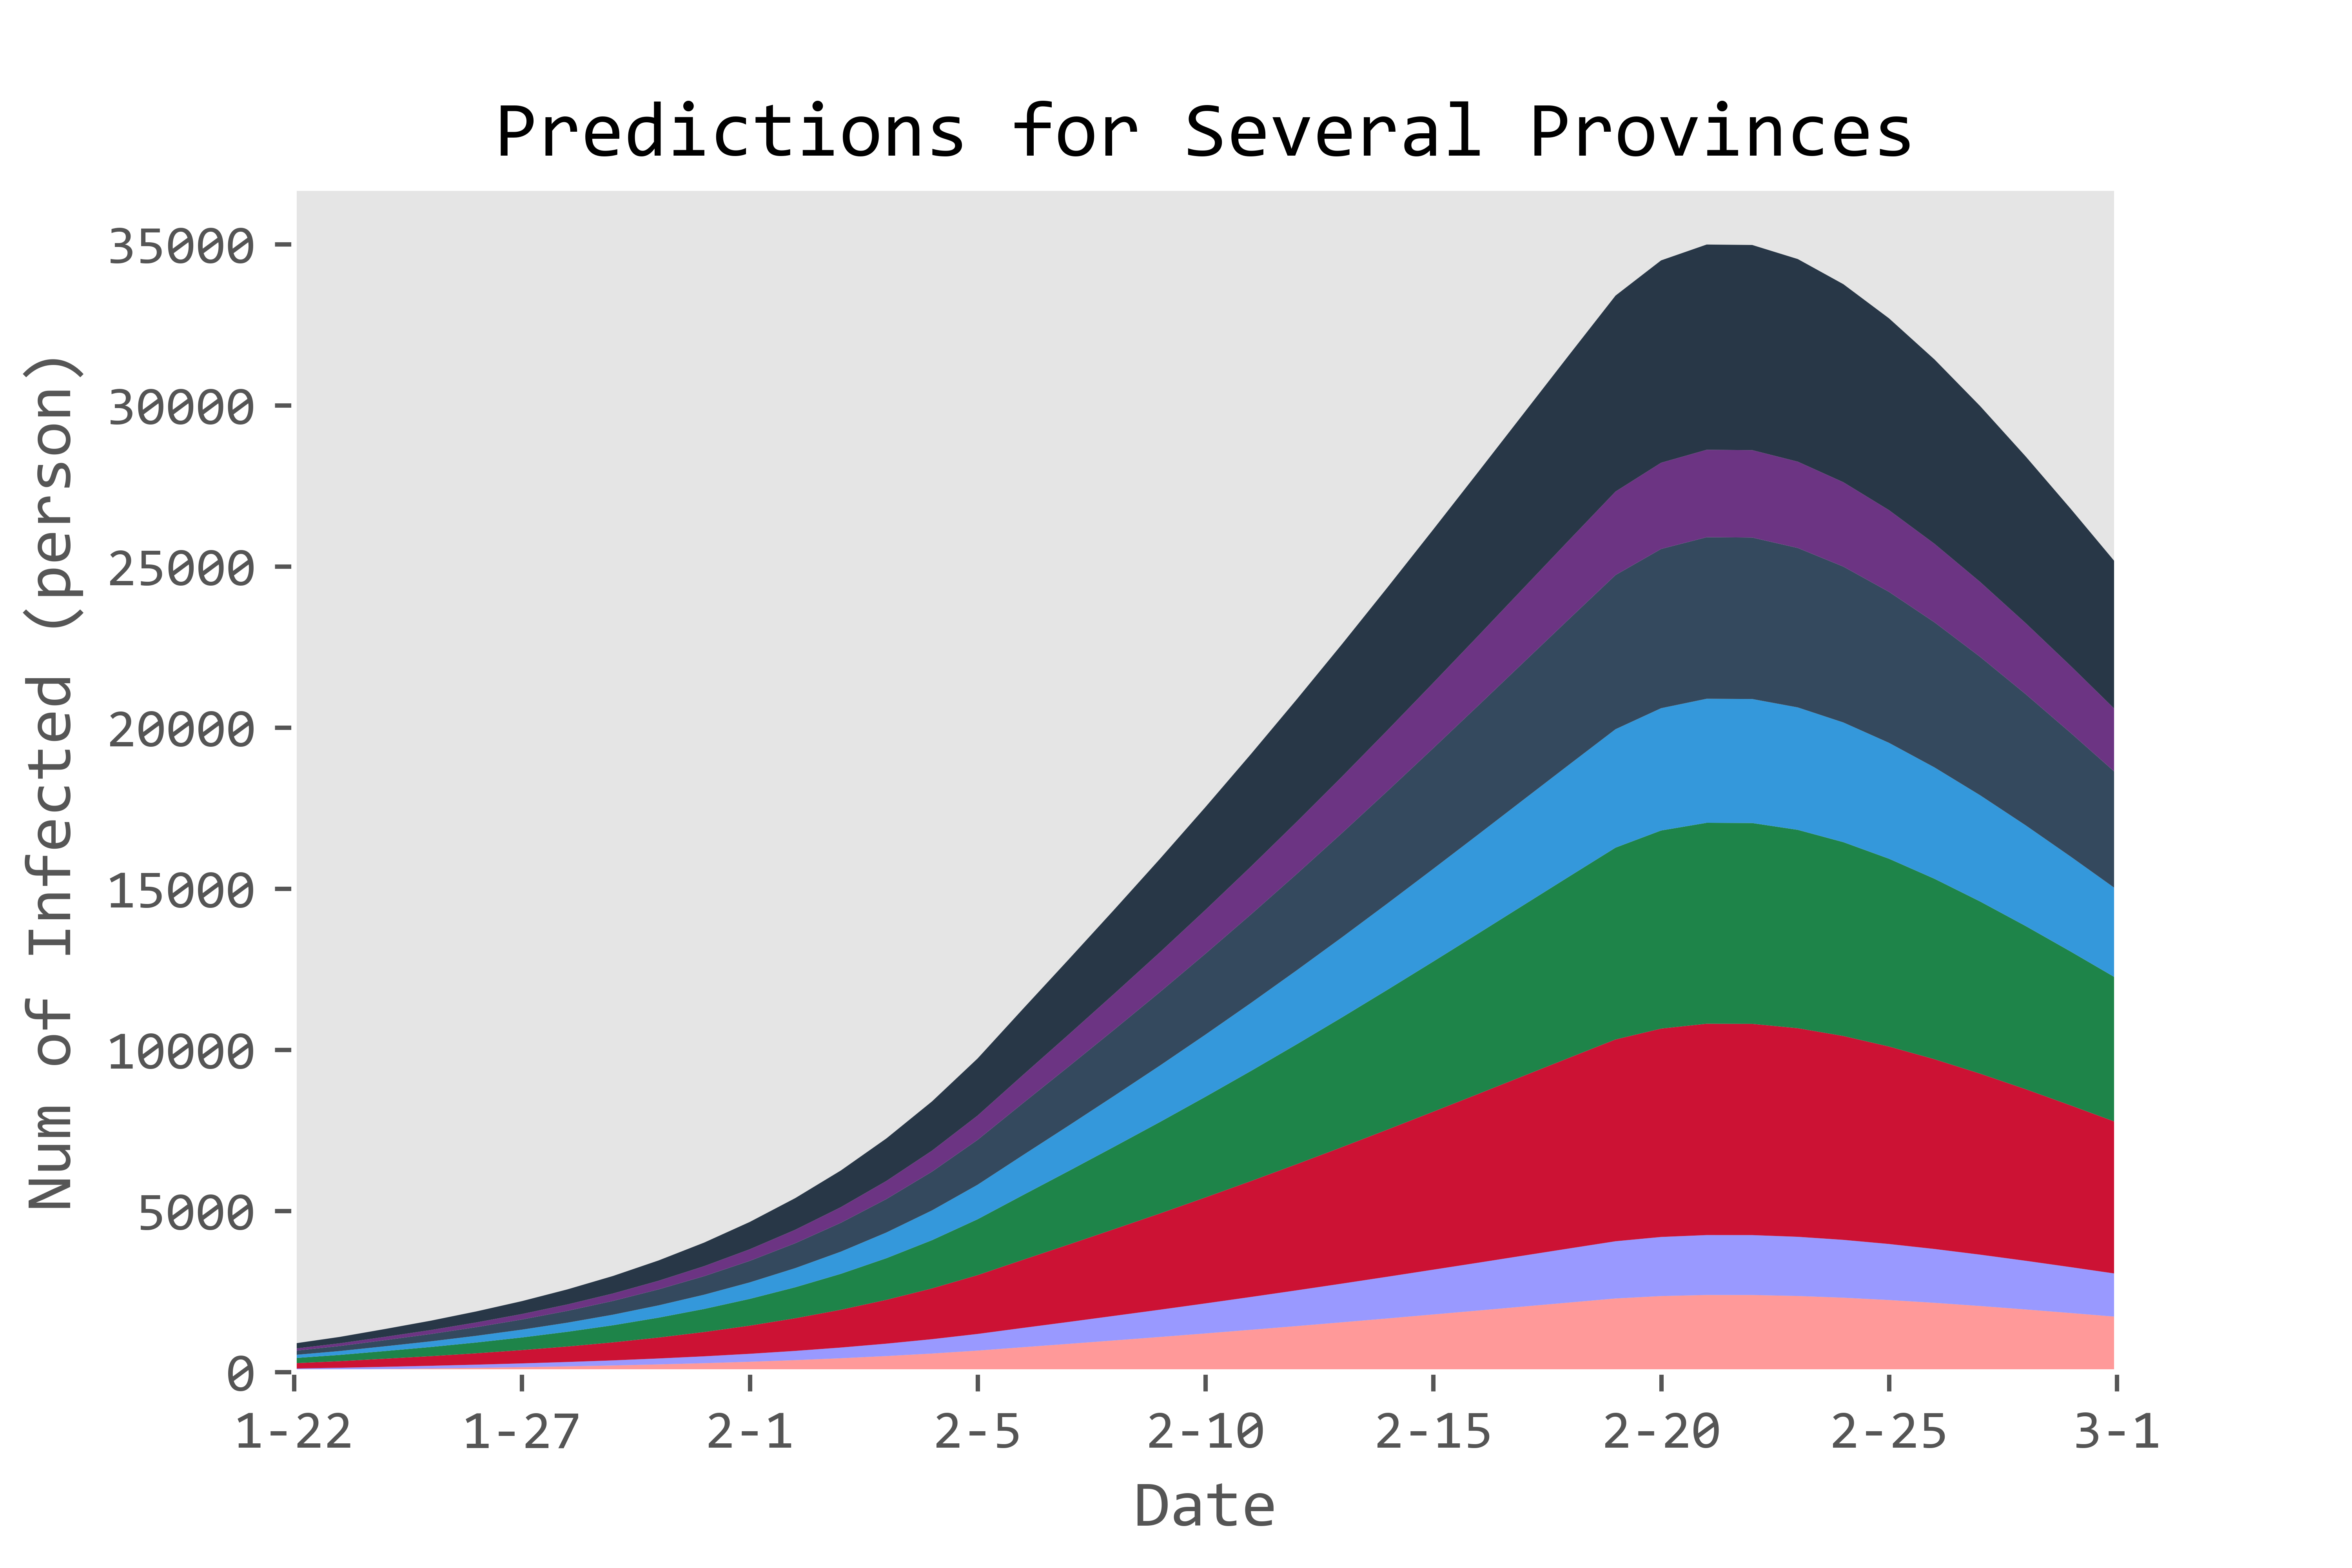
\includegraphics[width=\textwidth]{figure/Stack_Province_No_Holiday.png}
        \caption{\small{Without Extended Holiday}}
        \label{fig:Stack_No_Holiday}
    \end{subfigure}%
    \begin{subfigure}[b]{0.3\textwidth}
        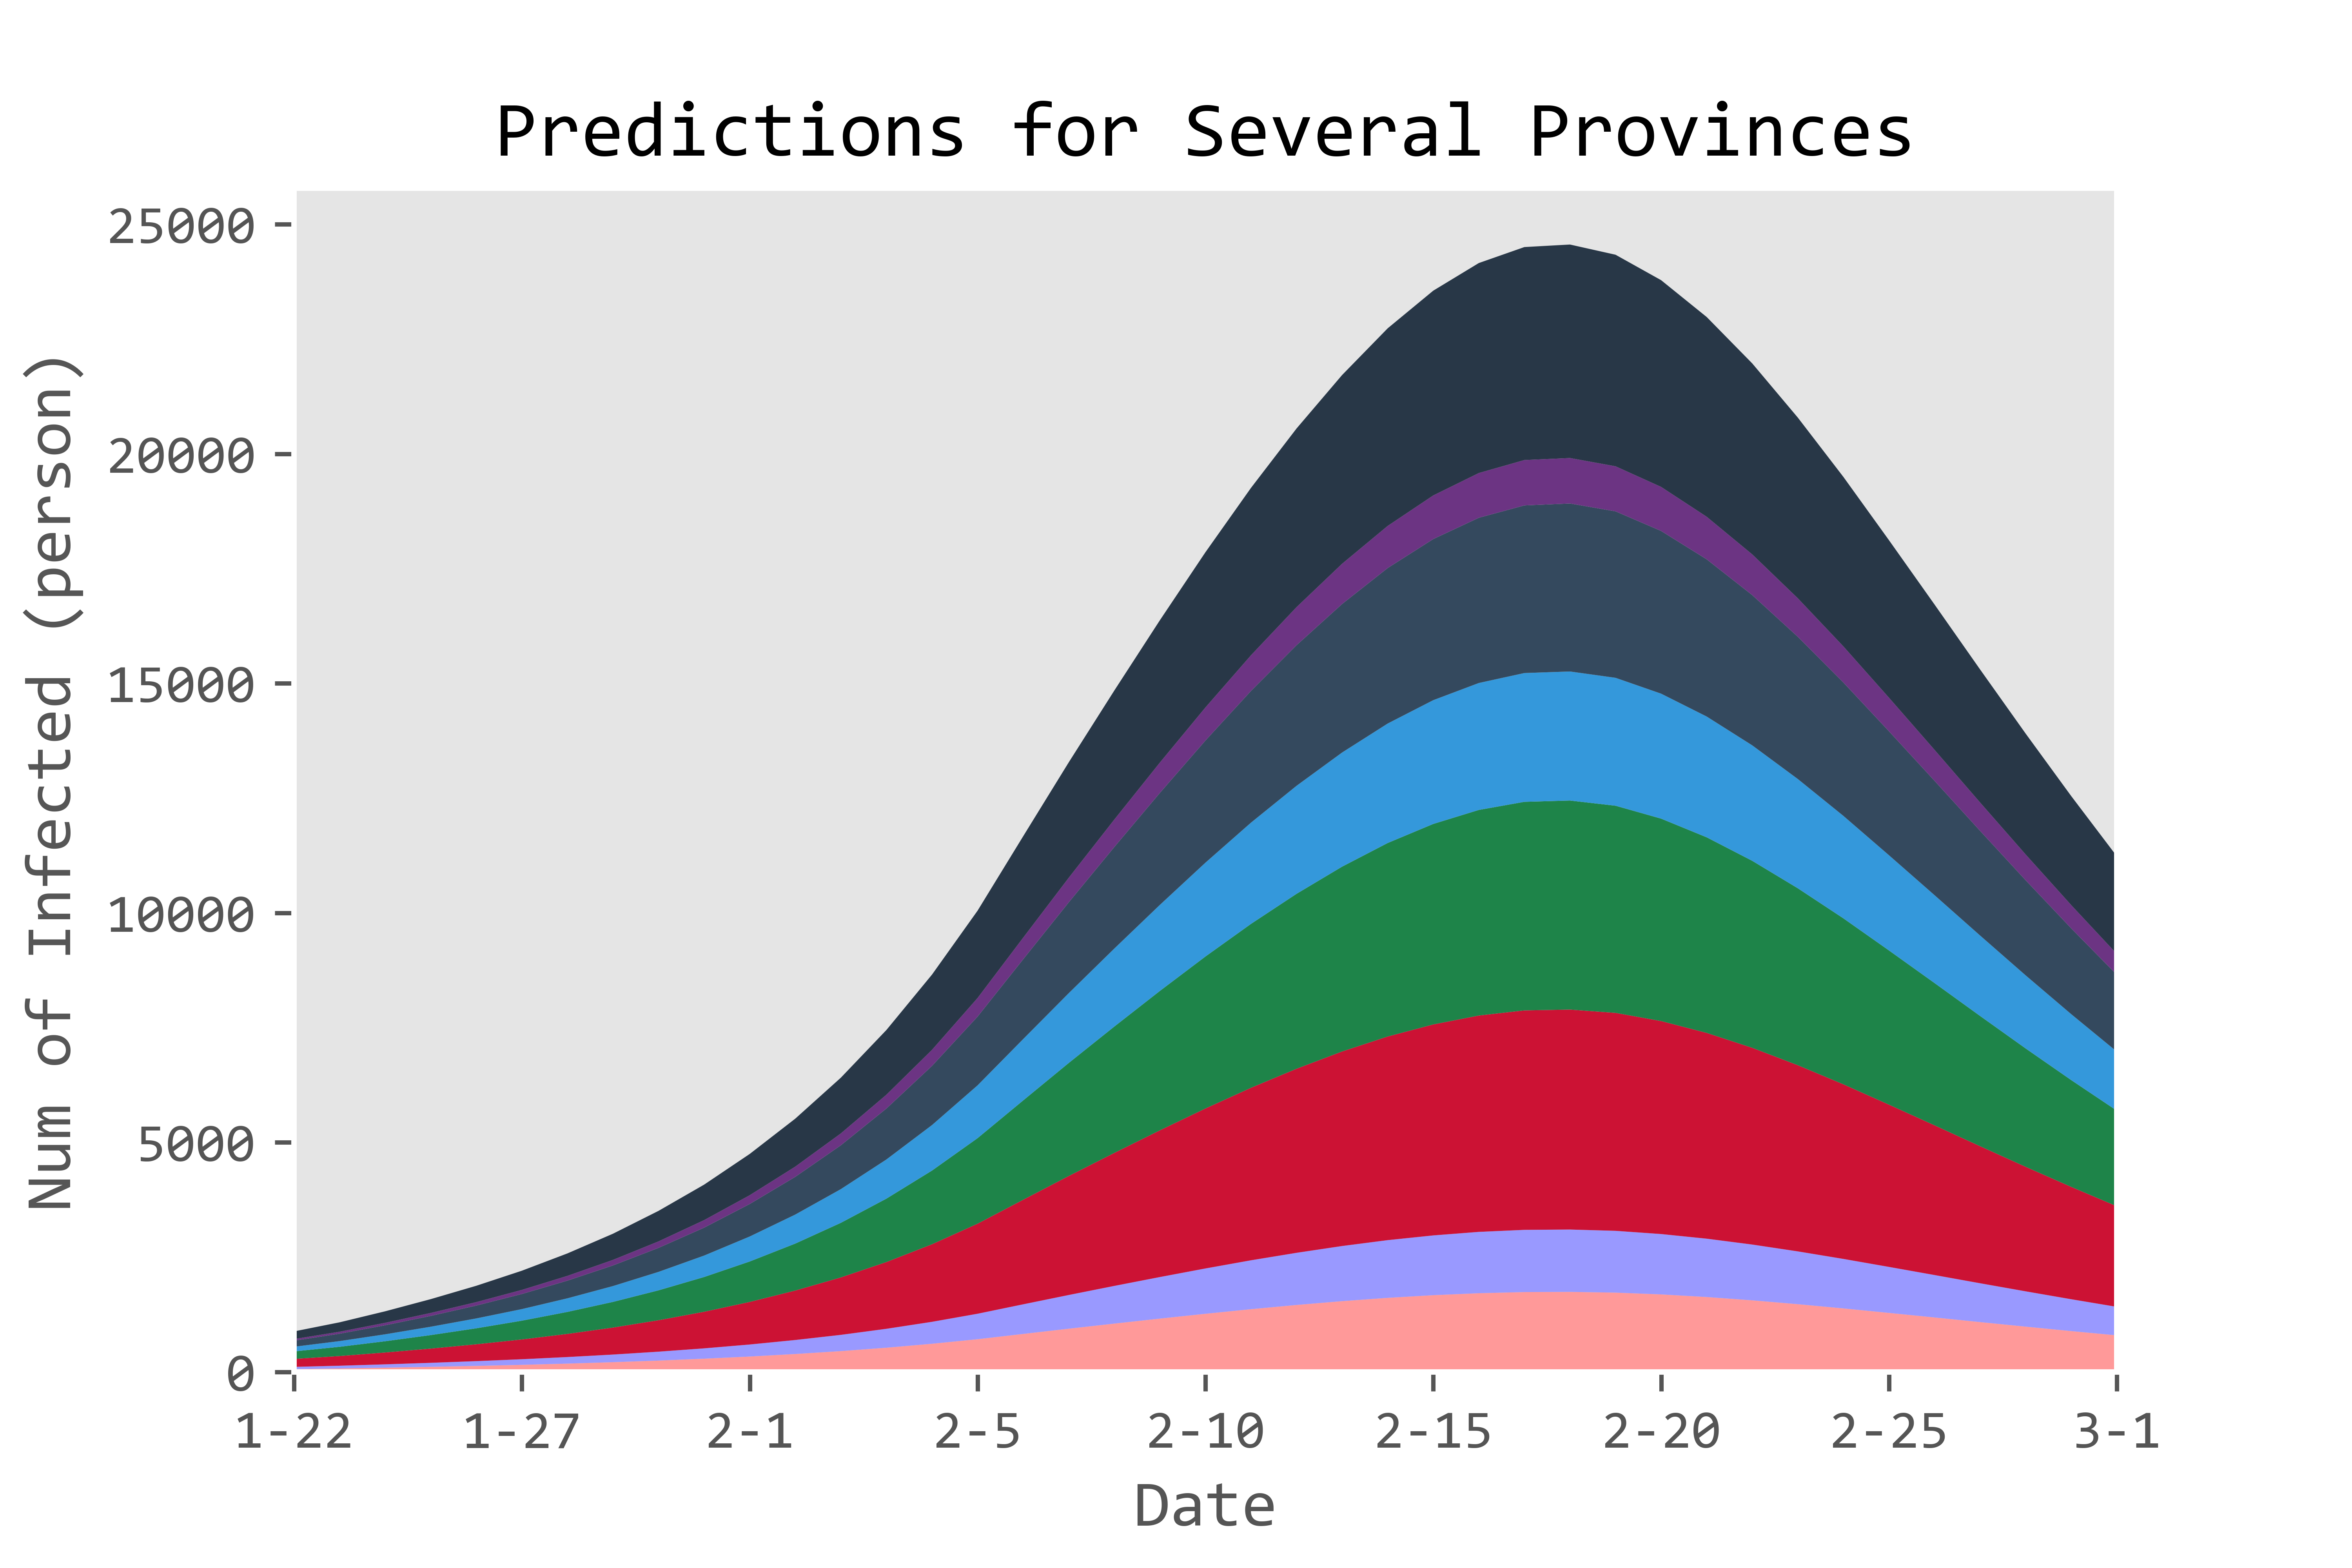
\includegraphics[width=\textwidth]{figure/Stack_Province_No_Geo_Restriction.png}
        \caption{\small{Without Traffic Restriction}}
        \label{fig:Stack_No_Tra_Rest}
    \end{subfigure}
    
    \caption{Predictions for Several Provinces in China}\label{fig:Stack}
\end{figure}

    Nevertheless, the reduction came with a cost. The lockdown --- encircling roughly 50 million people --- is unprecedented in scale and experts have questioned its ethics. Wuhan and its home province, Hubei, have borne the brunt of the epidemic as the sudden shutdown of transportation links into and around the area slowed the shipping of vital medical supplies. The scarcity partly contributed to the the difference in death rates of regions. The fatality rate in Wuhan is 4.1 percent and 2.8 percent in Hubei, compared to  0.17 percent elsewhere in mainland China. 
    
    Let's discuss the negative impacts in a larger scale. The Spring Festival break used to be a golden week, a boom for tourism and other tertiary industries. The tourism is in deep recession after coronavirus hit the whole country. It sharply slashed the revenue of tourism, over 70 billion dollars based on a report of 2019 by State Tourism Agency. The industry is also in depression. They have to delay resuming work to avoid the risk of getting employees infected. In final analysis, the pathogen put the whole economy under severe strain.

\subsection{Emergence of Various Factors}
If we put this problem into a bigger picture, many possible factors should be taken into consideration, including presence of secondary infection, discovery of effective treatment method and returning after Spring Festival.

\subsubsection{Presence of Secondary Infection}
There are two cases for secondary infection: non-permanent immunity and virus mutation. In case of non-permanent immunity, we return the recovered individuals to the susceptible stage immediately after their recovery, and thus our model is to become SEIS. In this case, the iterative equations (6)$\sim$(10) should be rewritten as following, ignoring the group of $R$:

\begin{align*}
    S_t^{(j)} &= P_t^{(j)} - E_t^{(j)} - I_t^{(j)} - D_t^{(j)} \\
    \Delta E_t^{(j)} &= E_{t+1}^{(j)} - E_t^{(j)} = hS_t^{(j)} + \left(f_{t,i}^{(j)} - f_{t,o}^{(j)} - \theta\right)E_t^{(j)} \\
    \Delta I_t^{(j)} &= I_{t+1}^{(j)} - I_t^{(j)} = \theta E_t^{(j)} - \left(r + k + f_{t,o}^{(j)} - f_{t,i}^{(j)}\right)I_t^{(j)} \\
    \Delta D_t^{(j)} &= D_{t+1}^{(j)} - D_t^{(j)} = kI_t^{(j)}
\end{align*}

We then implement our model according to the derivation above. The result is shown in Figure~\ref{fig:Twice_Inf}. As the number of recovered individuals is relatively small compared to the population of whole region, this type of secondary infection does not make a significant difference to our prediction.

In another case, the trend of epidemic situation will turn around immediately. The mutation of a virus means the increase of infecting chance $\gamma$ to $\gamma'$ for a susceptible individual to get infected. It at last leads to a rise in basic reproductive number $R_0$. We simulate the case in which we increase $\gamma$ by $0.015$ per day since Feb.10 until $\gamma'=1.0$, and plot the curve in Figure~\ref{fig:Mutation} compared with the original one. The consequence of virus mutation is much more serious, as the epidemic situation will be hard to control in a relatively long period of time.

\begin{figure}[htbp]
    \captionsetup{font={small}}
    \centering
        \begin{minipage}[c]{0.48\textwidth}
            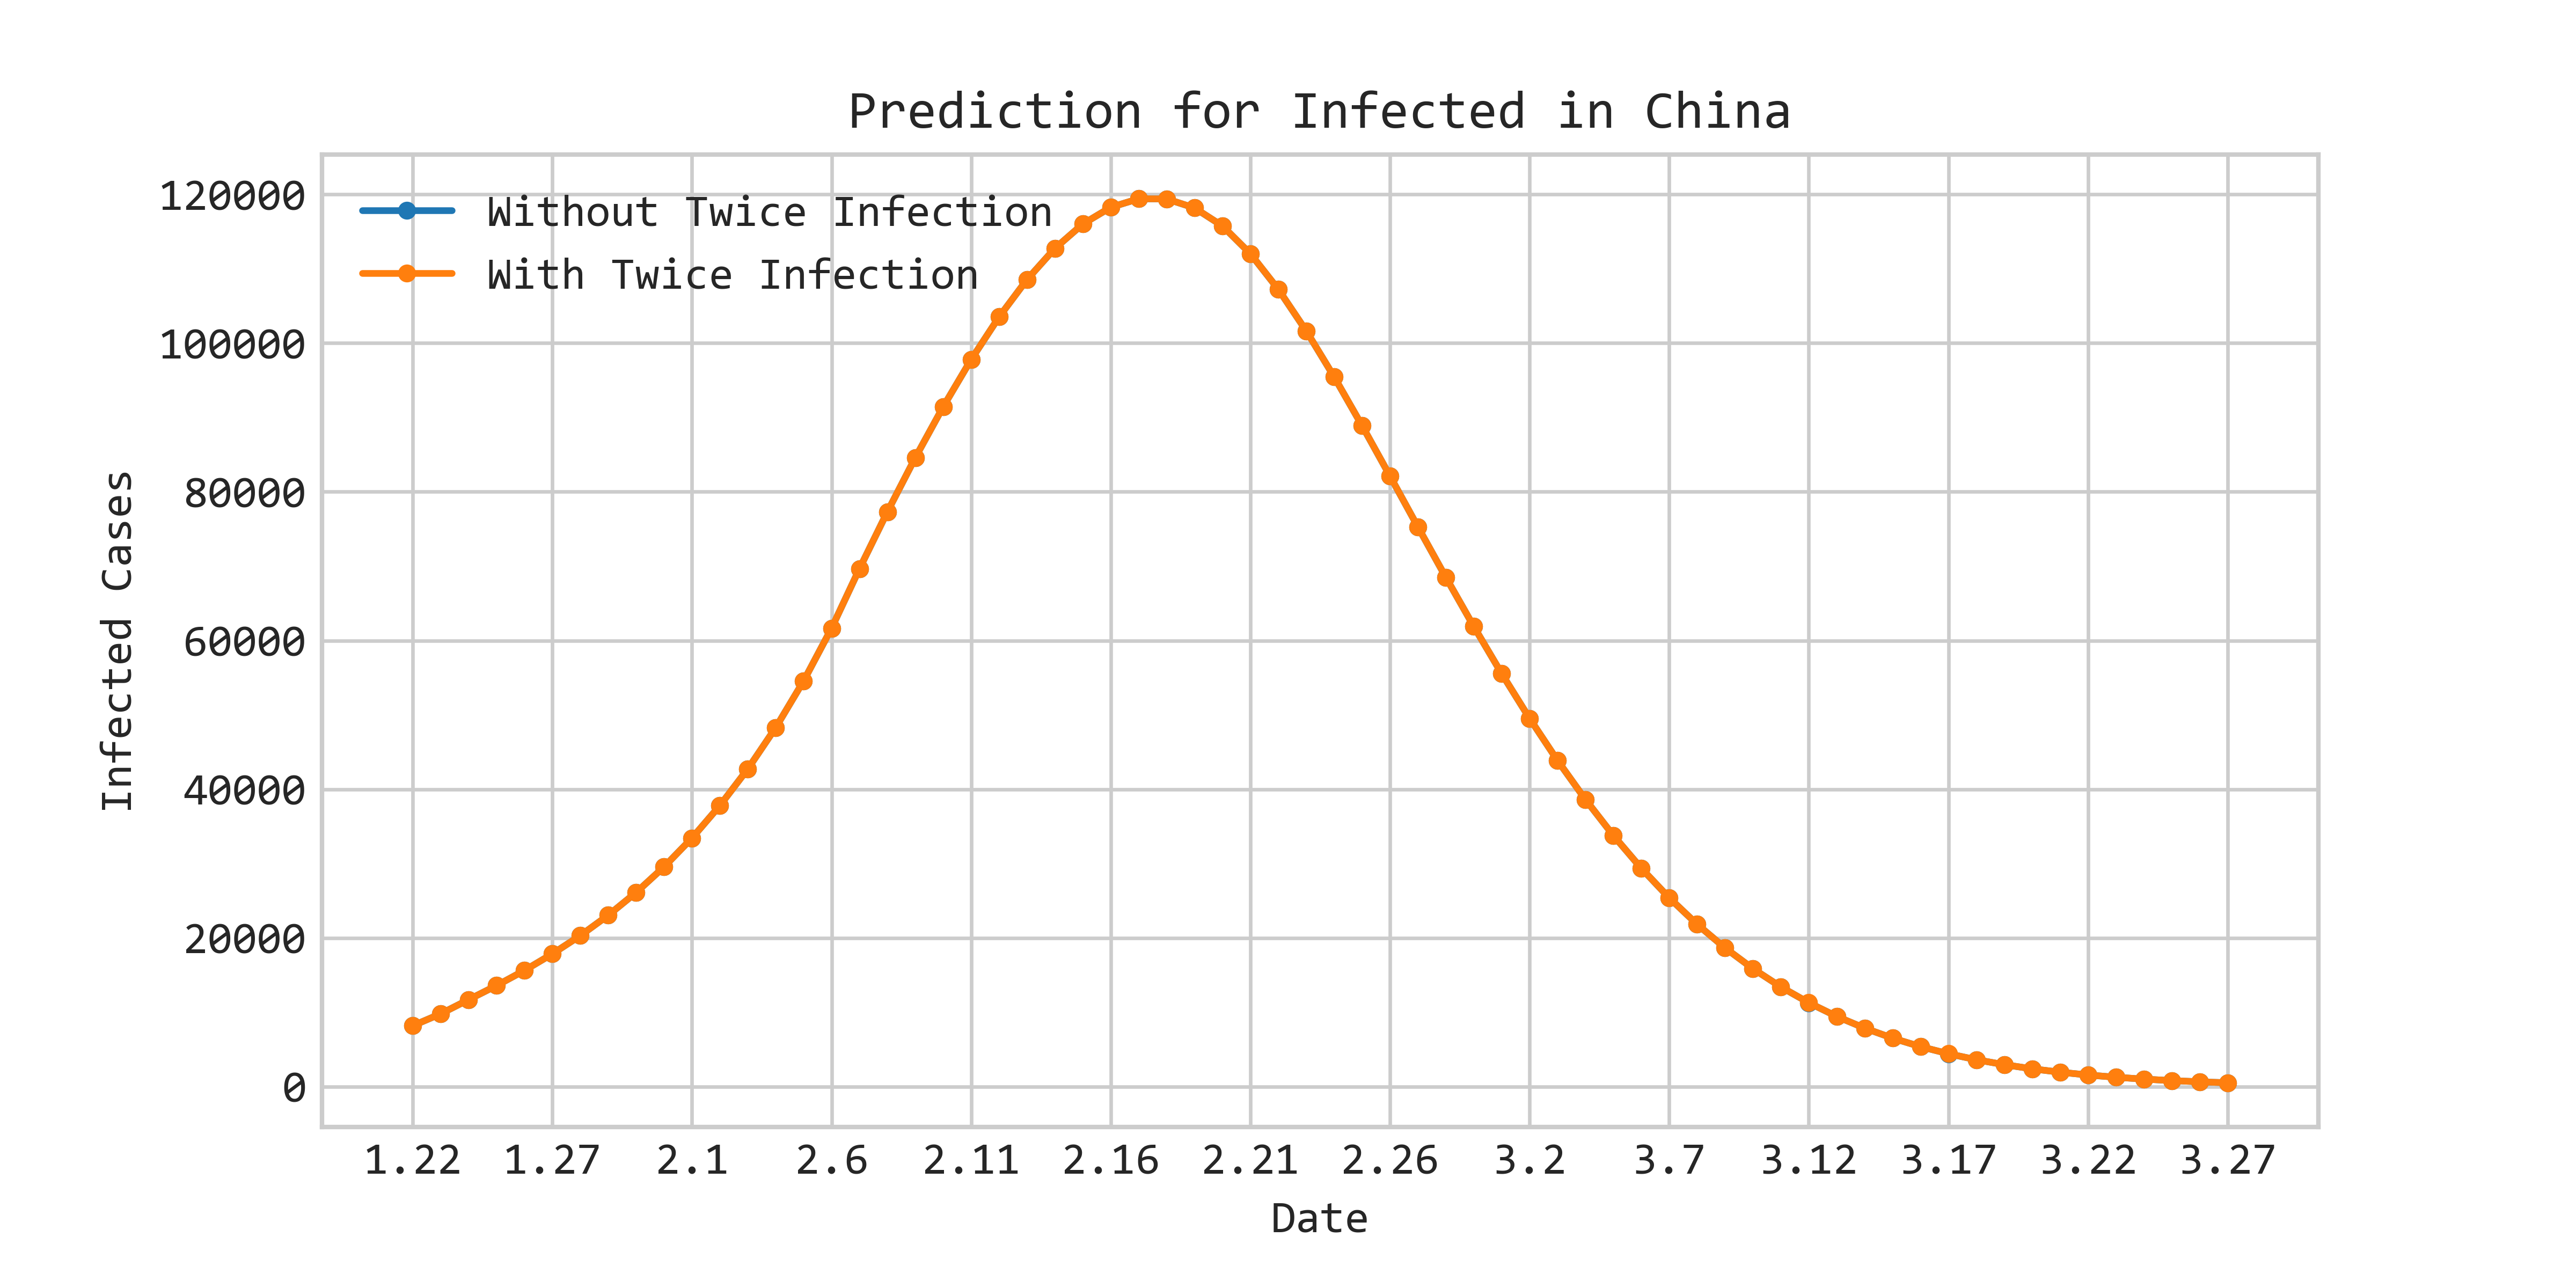
\includegraphics[width=1.0\textwidth]{053/figure/Prediction_With_Twice_Inf.png}
            \caption{Prediction with Twice Infection}
            \label{fig:Twice_Inf}
        \end{minipage}
        \begin{minipage}[c]{0.48\textwidth}
            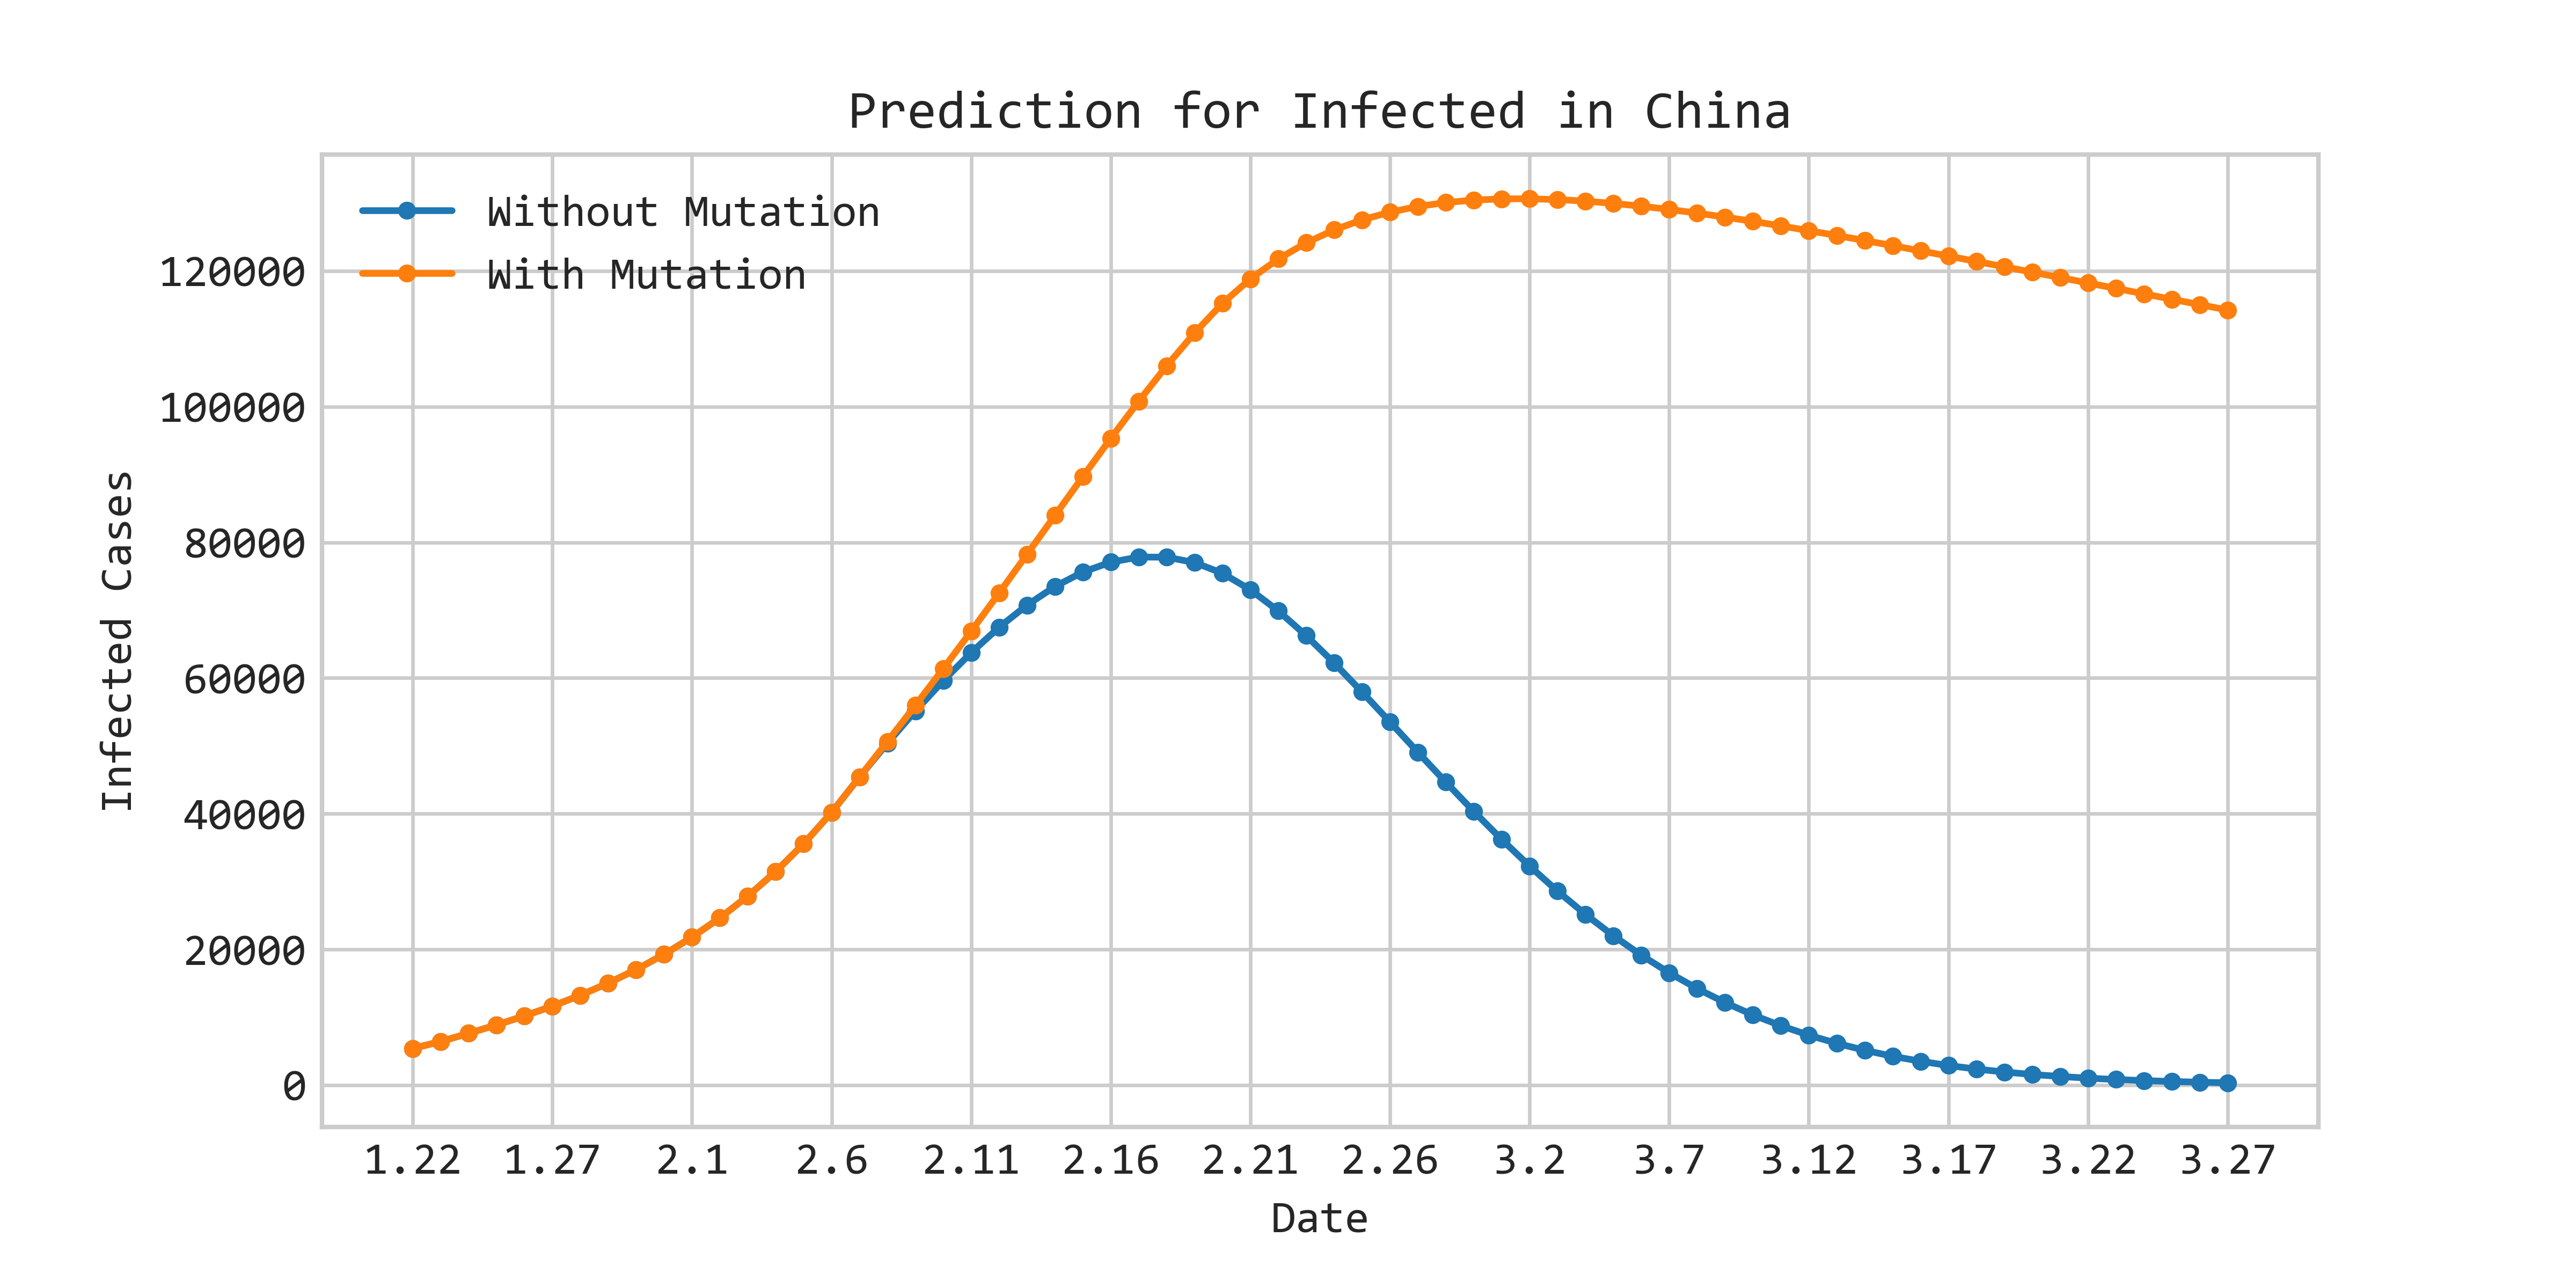
\includegraphics[width=1.0\textwidth]{figure/Prediction_With_Mutation.png}
            \caption{Prediction with Virus Mutation}
            \label{fig:Mutation}
        \end{minipage}
\end{figure}

\subsubsection{Discovery of Effective Treatment Method} \label{subsubSec:treat}
When an effective treatment method is developed for a certain disease, the major and direct result will be a sharp rise in its recover ratio. Therefore, we assume the recover rate $r$ of 2019-nCoV will increase to 0.05, which means our treating efficiency is ten times as before.

We rerun our model with $r$ raised at different timestamps, and thus obtain a curve showing the influence of new treatment and its timing in Figure~\ref{fig:New_Med}.


The influence of effective treatment is clear: the earlier it is discovered, the earlier China can control the situation and the less total infections. More importantly, the shortage of test kits is a bigger issue. If we don't have the actual number of infections, then we may make the wrong prediction and underestimate the situation.

\begin{figure}[htbp]
    \captionsetup{font={small}}
    \centering
        \begin{minipage}[c]{0.48\textwidth}
            \includegraphics[width=1.0\textwidth]{053/figure/Prediction_New_Medicine.png}
            \caption{Prediction with New Medicine}
            \label{fig:New_Med}
        \end{minipage}
        \begin{minipage}[c]{0.48\textwidth}
            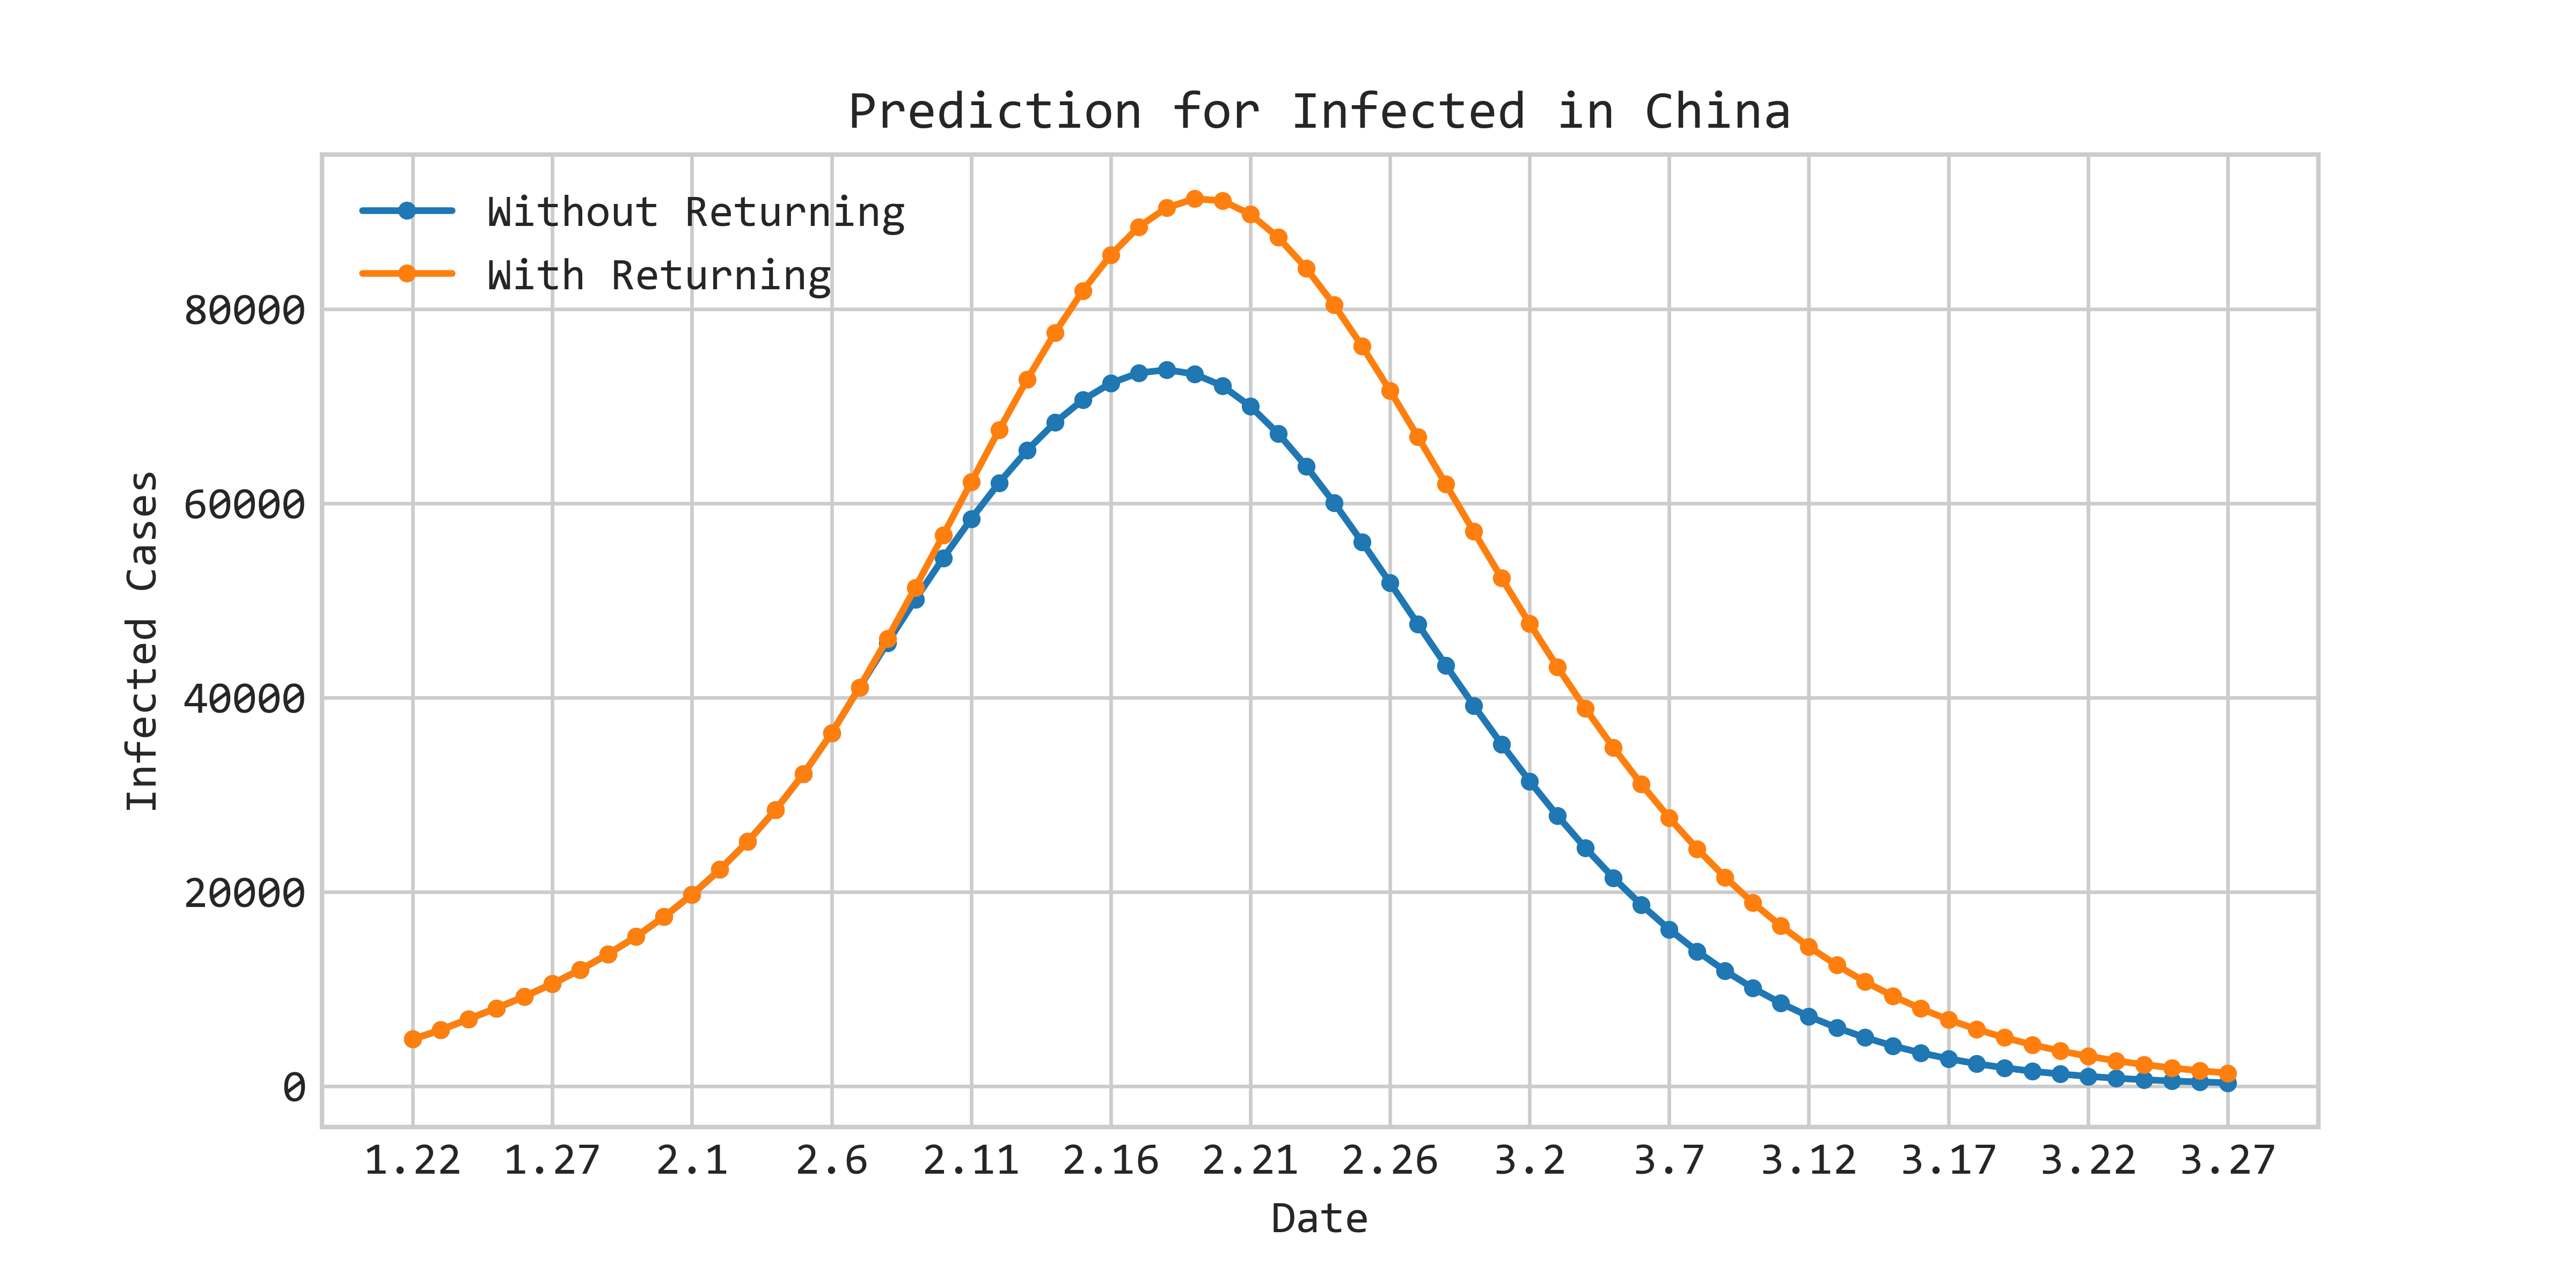
\includegraphics[width=1.0\textwidth]{053/figure/Prediction_WithReturning.png}
            \caption{Prediction with Returning to Work }
            \label{fig:Return}
        \end{minipage}
\end{figure}

\subsubsection{Returning after Spring Festival}
The traditional transportation in China also involves the large-scale returning after Chinese New Year, which means another peak of population flow between regions. Because of the control measures of Chinese government, the traffic pulse has been buffered. To restore its impact on the spread of epidemic, we let $a$ (thus $h$) rise a bit after the Spring Festival and then level down to the same value as our original model. Figure~\ref{fig:Return} exhibits the influence of the returning rush.

From the picture, we can see that the big returning after festival reasonably leads to a higher peak of infections, which also proves the effectiveness of our countries' measures.

To sum up, all signs point to the possibility that WHO will terminate the PHEIC earlier than 3 months routine review.

\section{Model Analysis} \label{Sec:analysis}
\subsection{Sensitivity Analysis}
In Section~\ref{subSec:Para}, we chose values for some parameters in our model according to recent reports and statistics. Here we are going to discuss the sensitivity of them, utilizing the reproductive number $R$ defined in Section~\ref{subsubSec:R0}. Before detailed discussion, we formalize the sensitivity $S(x)$ of a variable $x$ in this article as following:

\textbf{Definition} \textit{Given the peak of infections $I_p(x = x_0)$, the sensitivity of variable $x$ at $x = x_0$ is:}
\begin{equation*}
S_x(x_0) = \left[\left(\frac{{\rm d}I_p(x)}{I_p(x)}\right) \middle/ \left(\frac{{\rm d}x}{x}\right)\right]\bigg|_{x = x_0} = \left[\left(\frac{{\rm d}I_p(x)}{{\rm d}x}\right)\left(\frac{x}{I_p(x)}\right)\right]\bigg|_{x = x_0}
\end{equation*}

Since the peak is only accessible through numeric simulation, we take its difference as its differential, just as what we did with the equations in Section~\ref{subsubSec:eqn}.

\subsubsection{The Sensitivity of $b$ and $\gamma$}
These two parameters are closely related to the reproductive number $R$, and thus have huge impacts on the peak of  infections as shown in Figure~\ref{fig:Sens_b} and~\ref{fig:Sens_gama}. We also evaluate their sensitivity and impact on the reproductive number $R$ numerically:

\begin{align*}
    S_b(b = 0.6) &= \frac{134000 - 40000}{0.65 - 0.55} \times \frac{0.6}{74000} \approx 7.62\\
    S_{\gamma}(\gamma = 0.75) &= \frac{120000 - 45000}{0.8 - 0.7} \times \frac{0.75}{74000} \approx 7.60 \\
    \frac{{\rm d}R}{{\rm d}b} &= \frac{\gamma a P}{\lambda} = 5.25 \\
    \frac{{\rm d}R}{{\rm d}\gamma} &= \frac{a b P}{\lambda} = 4.2
\end{align*}

Here we can summarize an important inference: The parameters in SEIR model tend to have high sensitivity since tiny changes could lead to a large difference in the reproductive number $R$. This can be proved on the contrary by looking into the sensitivity of total population $P$: Similarly we have $\frac{{\rm d}R}{{\rm d}P} = \frac{\gamma a b}{\lambda} < 10^{-6}$, so even if we double $P$ to more than $2 \times 10^7$, the infections are quite the same as before.

\begin{figure}[H]
    \centering
    \begin{subfigure}[t]{0.45\textwidth}
        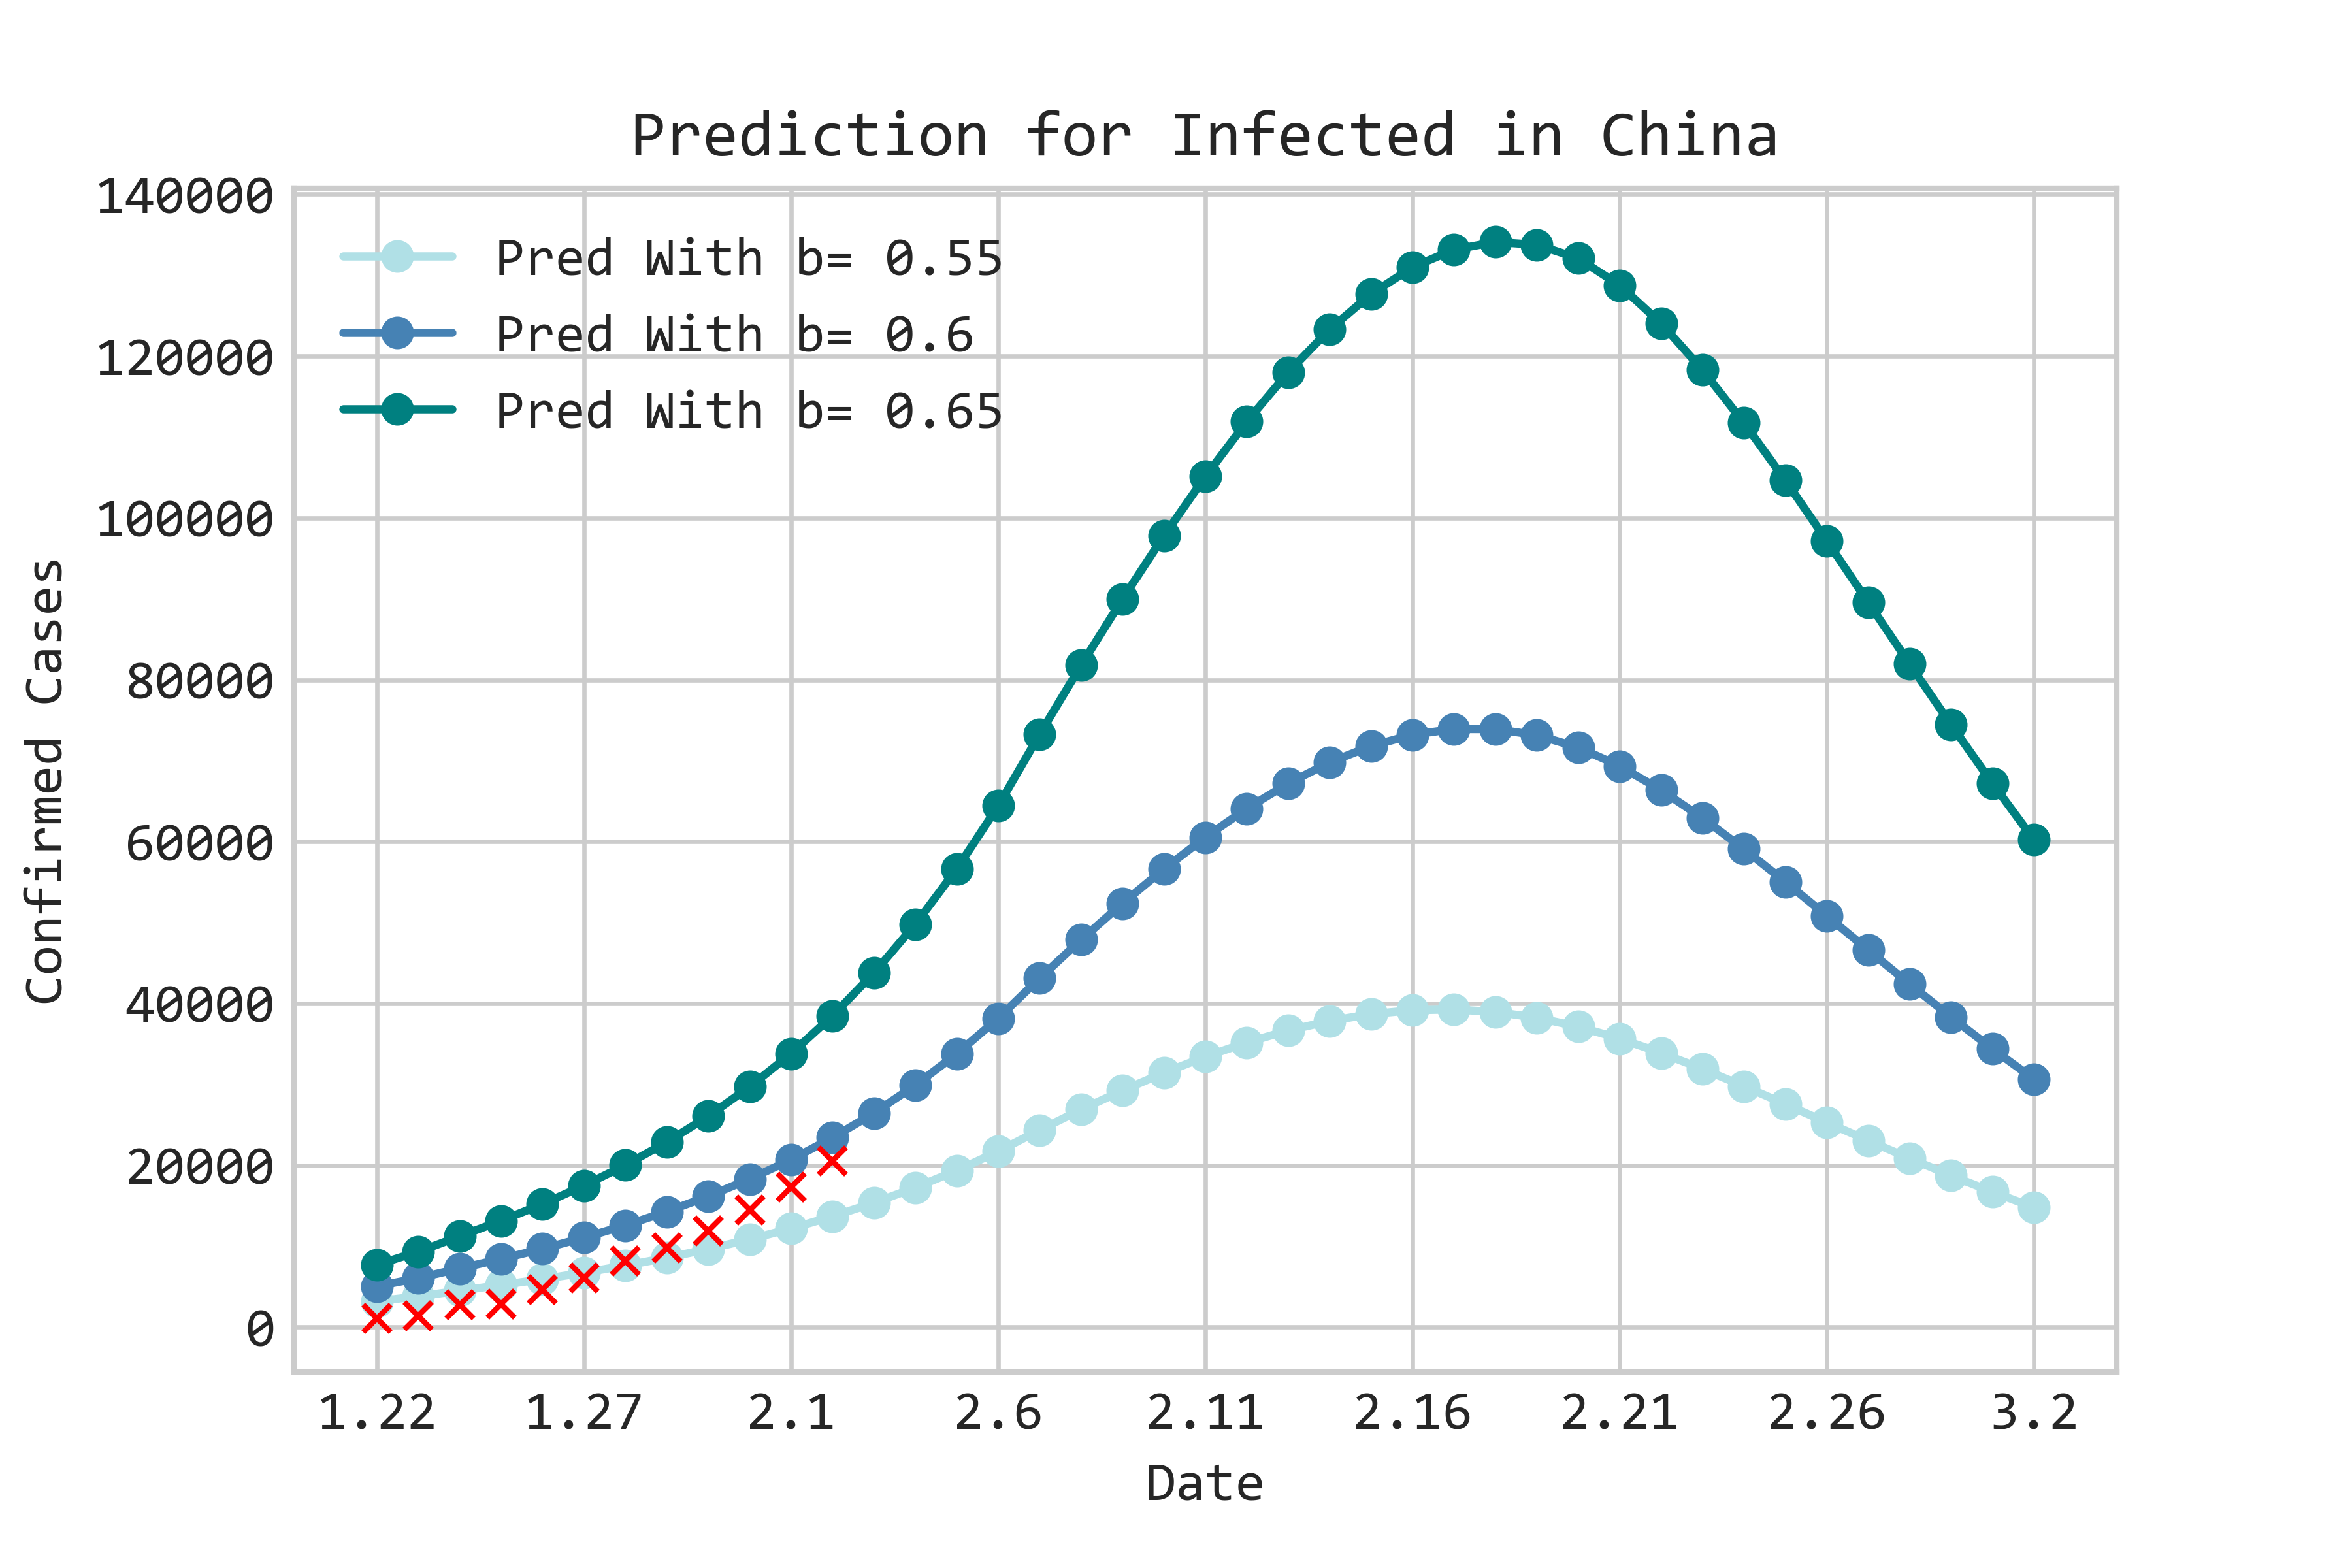
\includegraphics[width=1.0\textwidth]{053/figure/Sens_b.png}
        \caption{Sensitivity of $b$}
        \label{fig:Sens_b}
    \end{subfigure}
    \begin{subfigure}[t]{0.45\textwidth}
        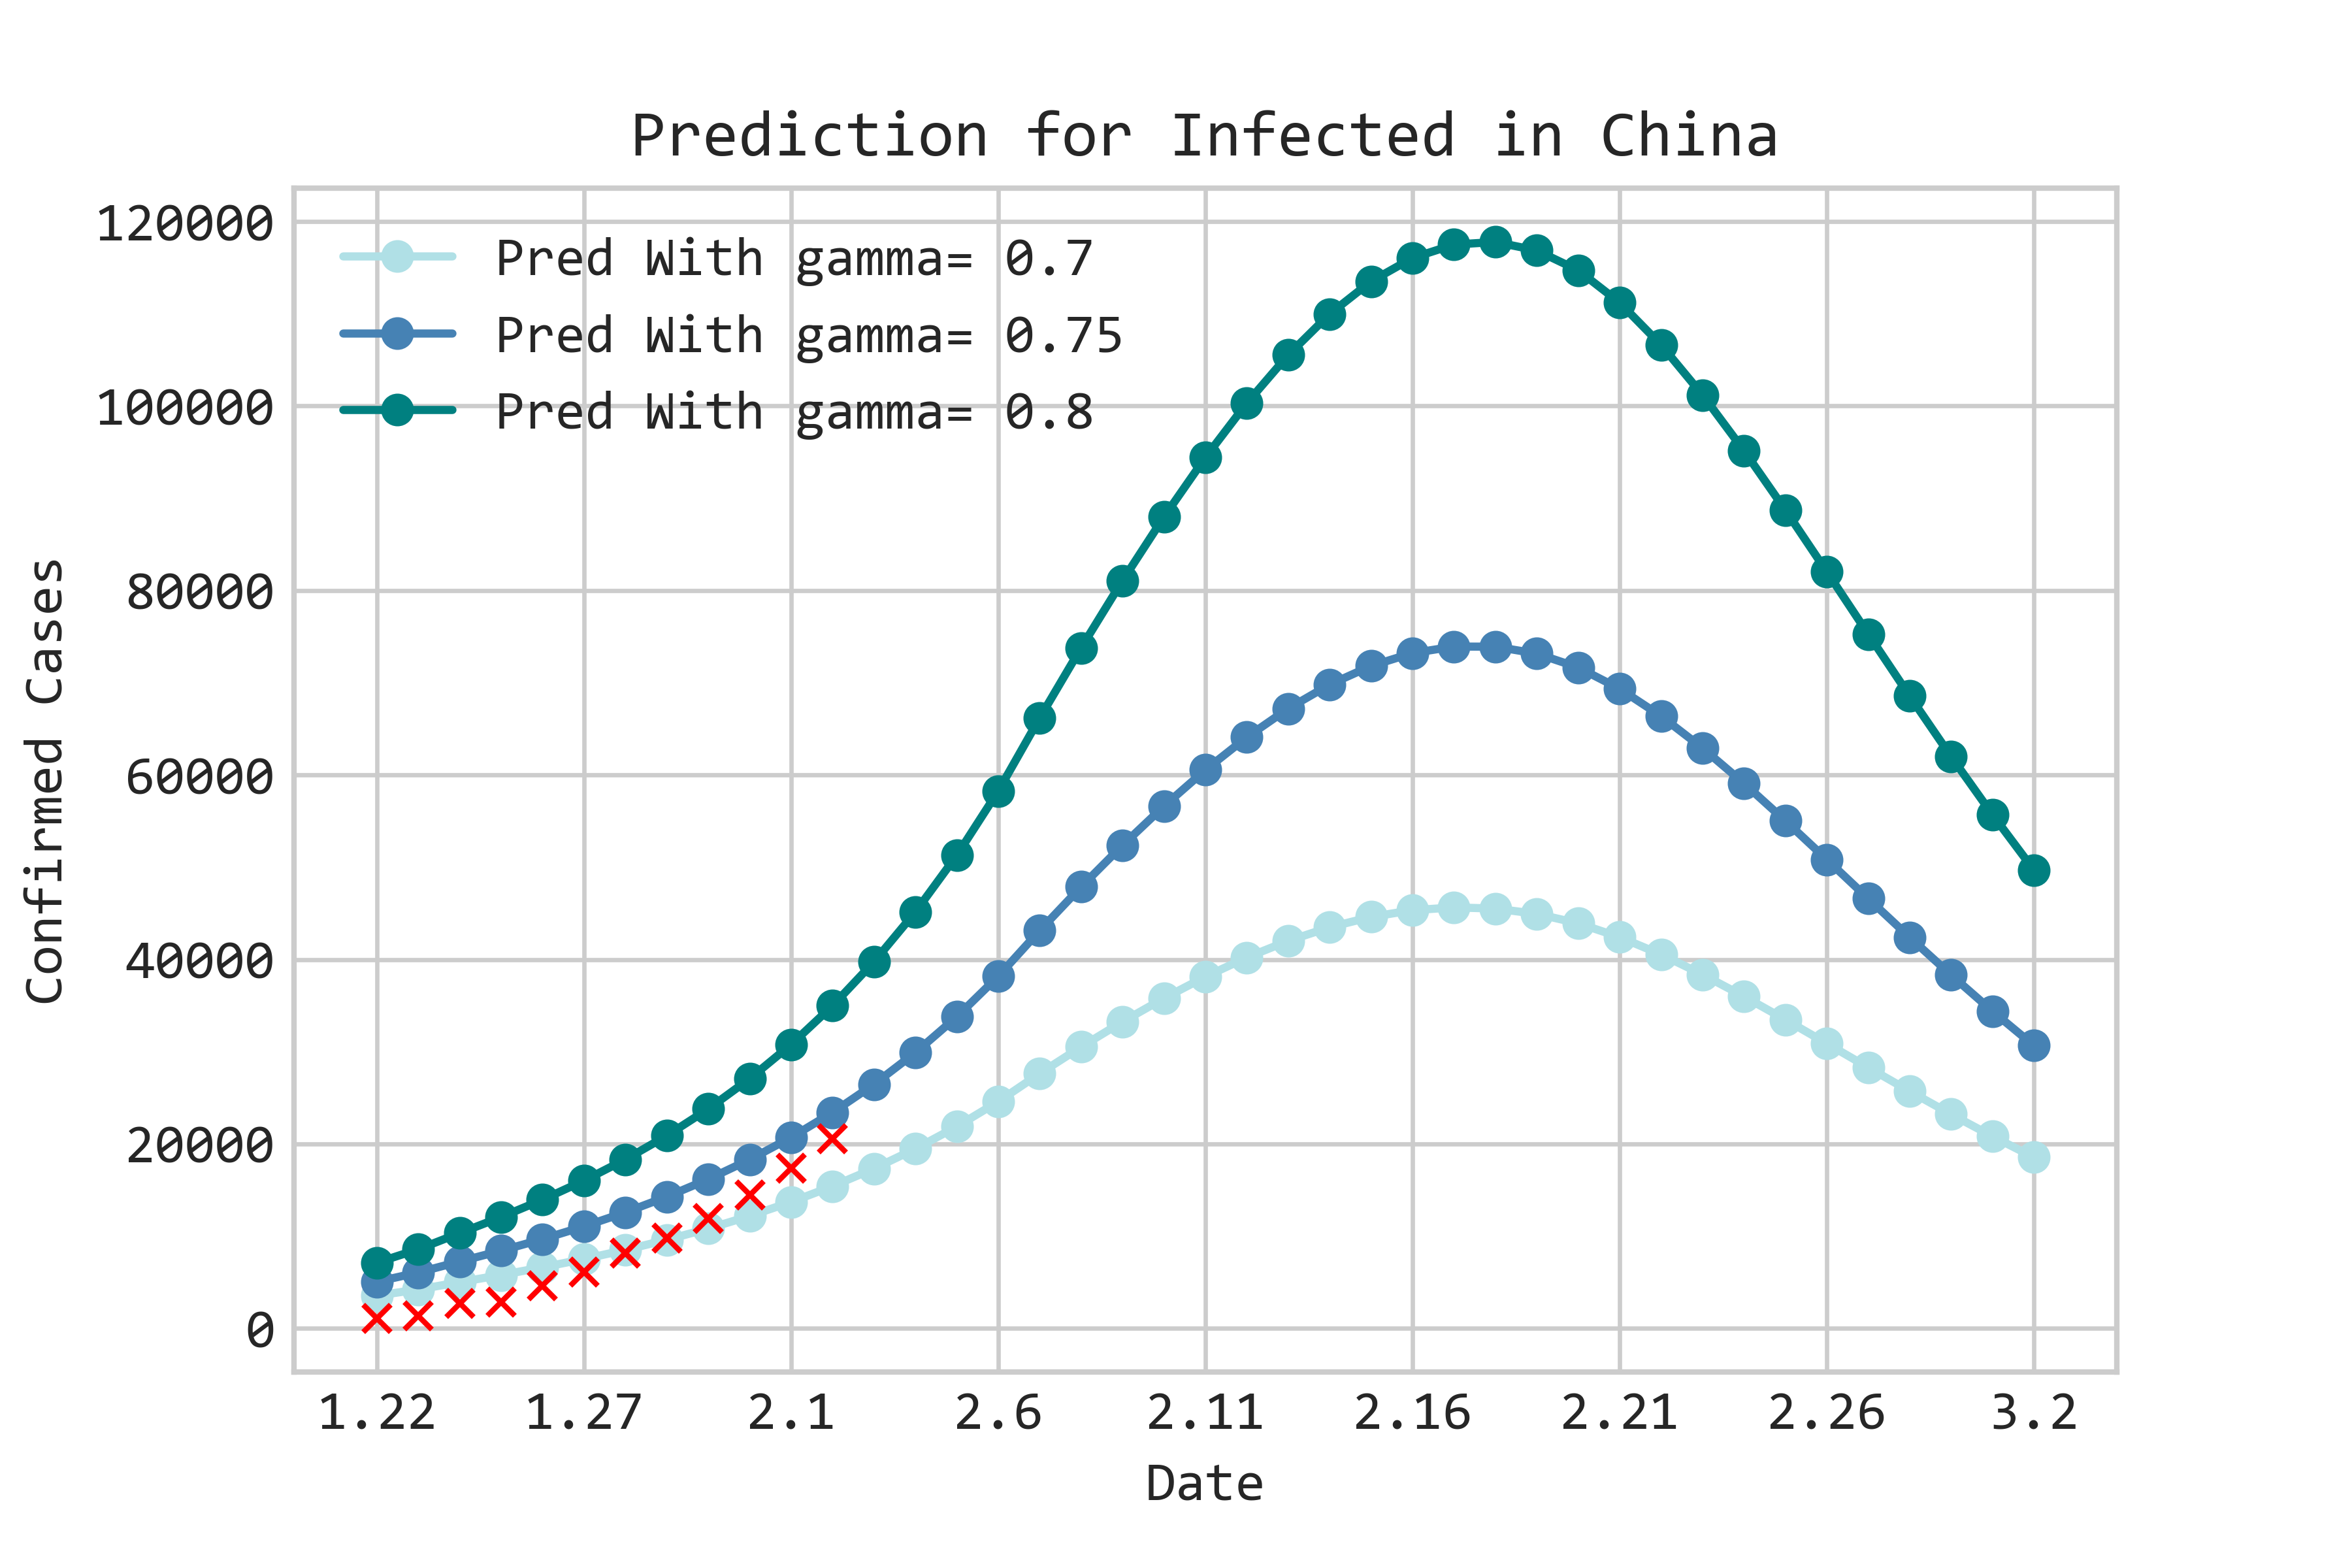
\includegraphics[width=1.0\textwidth]{053/figure/Sens_gamma.png}
        \caption{Sensitivity of $\gamma$}
        \label{fig:Sens_gama}
    \end{subfigure}
    \\
    \begin{subfigure}[t]{0.45\textwidth}
        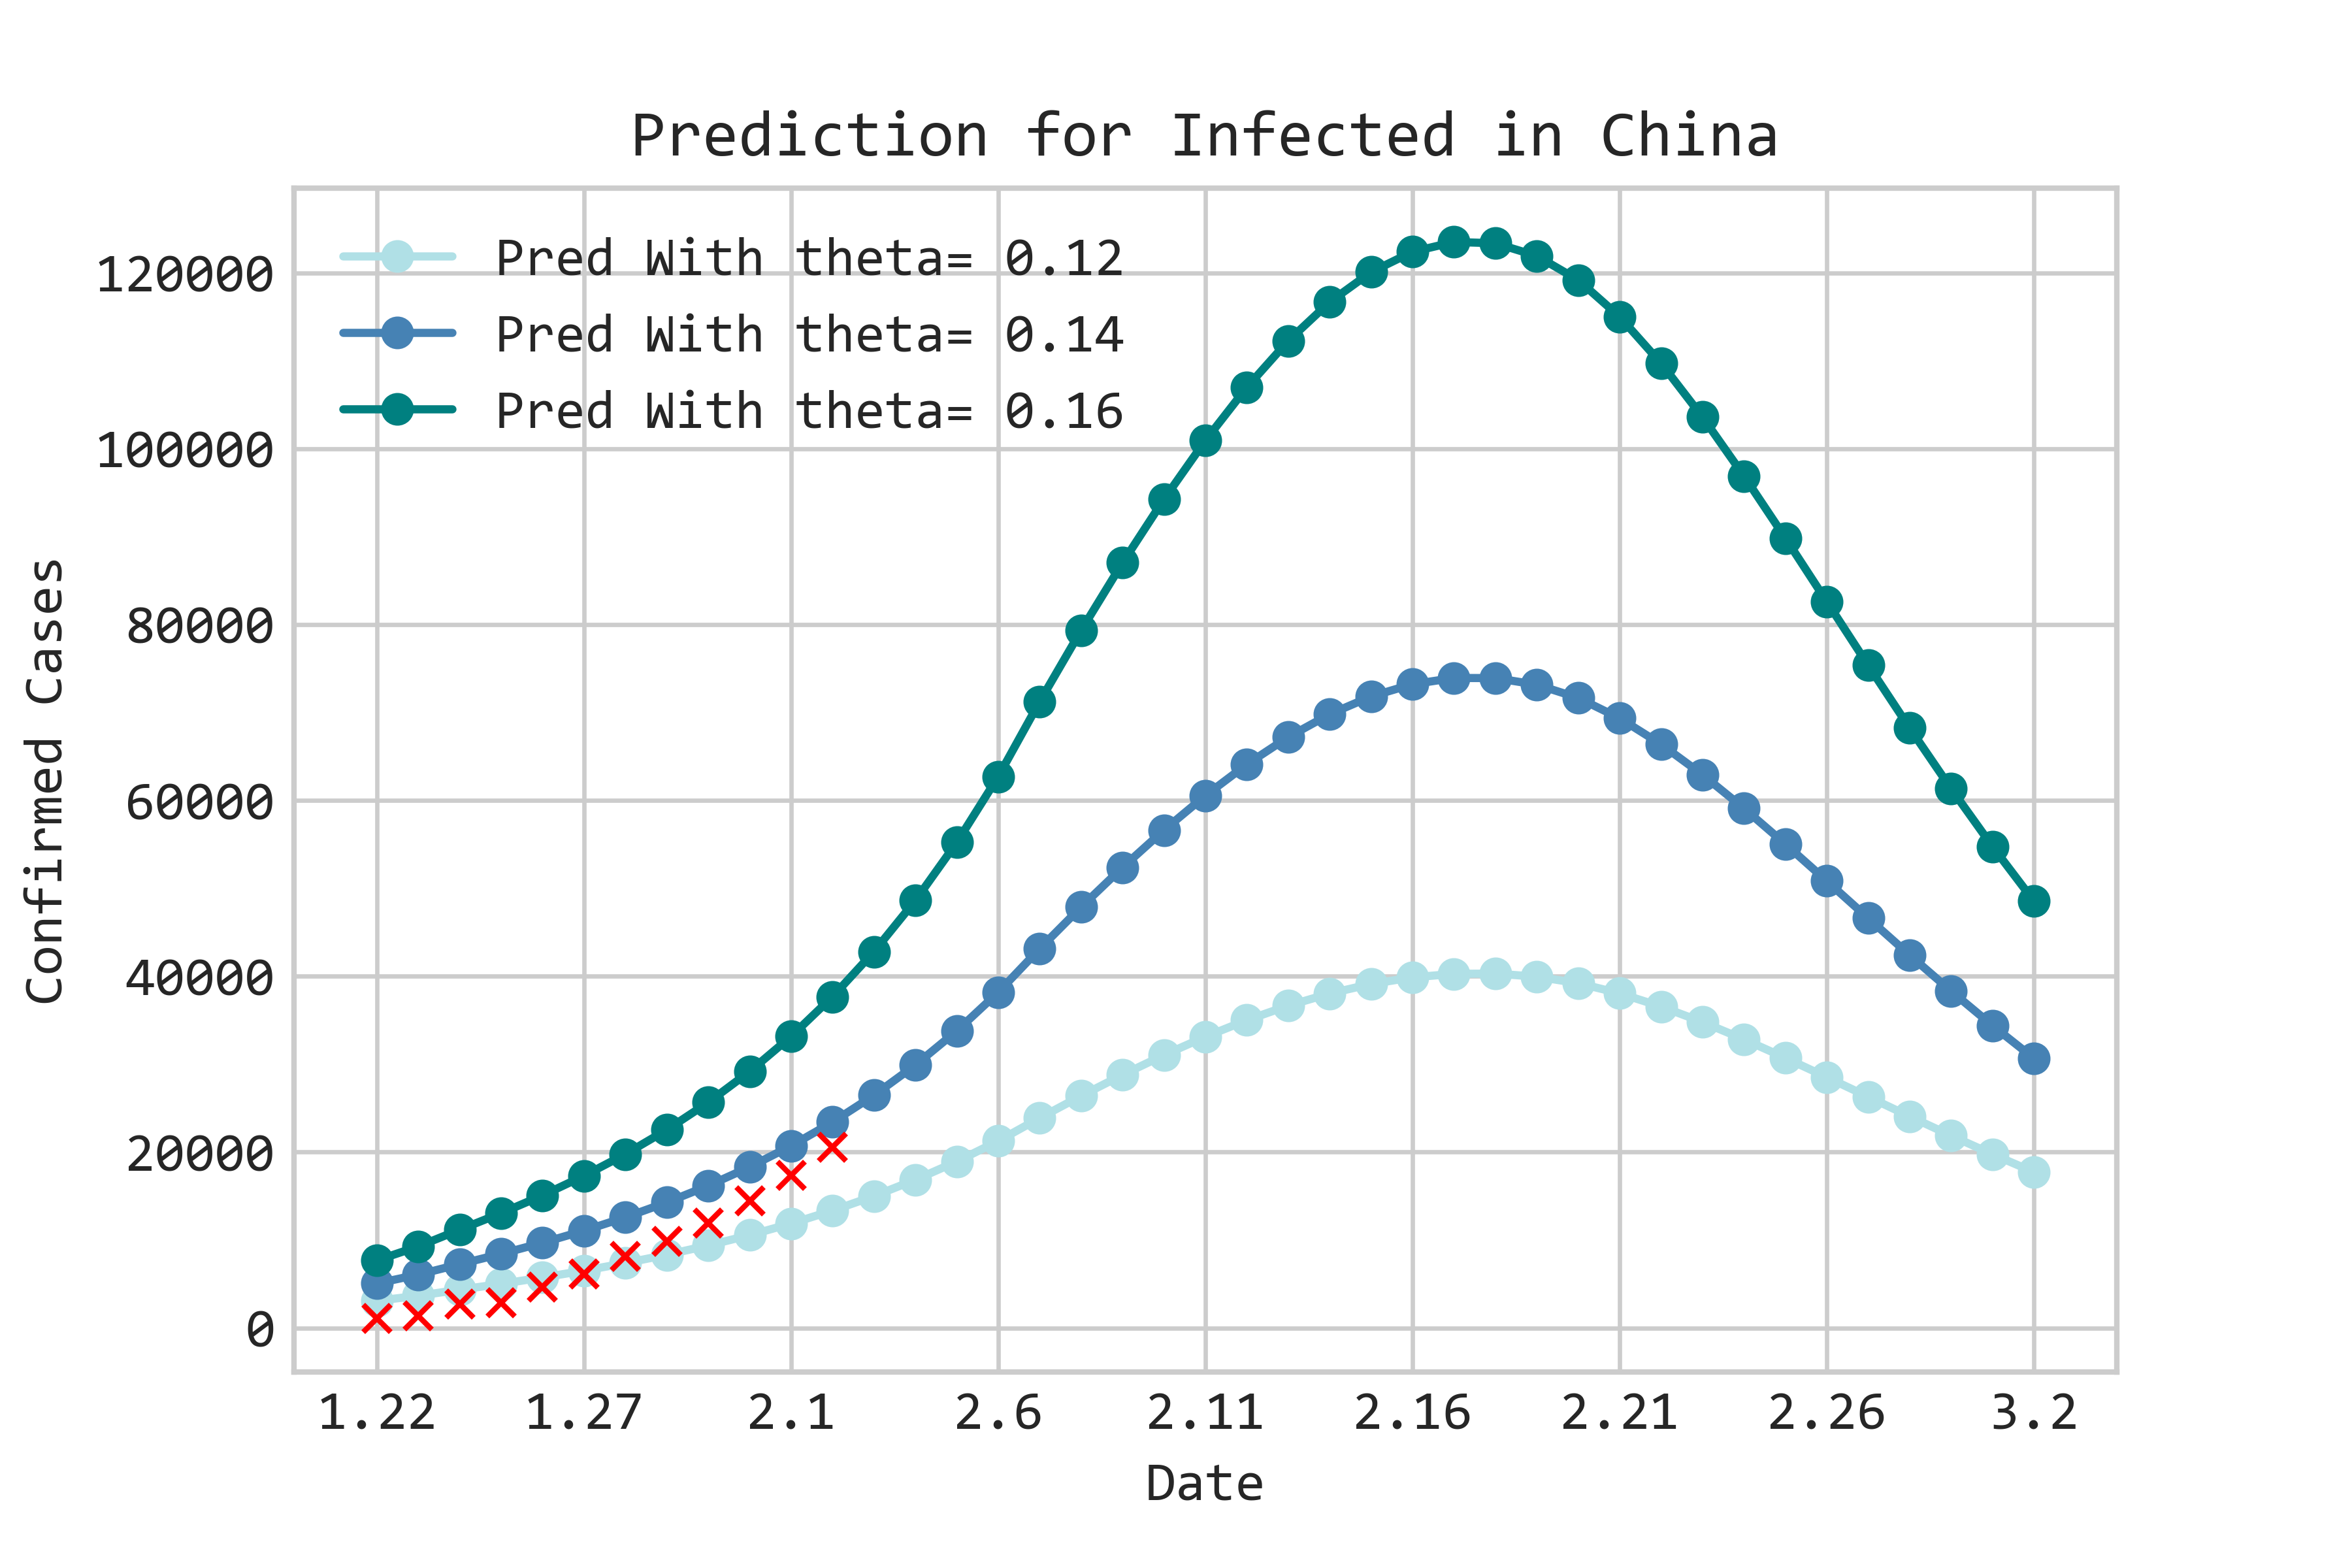
\includegraphics[width=1.0\textwidth]{053/figure/Sens_theta.png}
        \caption{Sensitivity of $\theta$}
        \label{fig:Sens_thita}
    \end{subfigure}
    \begin{subfigure}[t]{0.45\textwidth}
        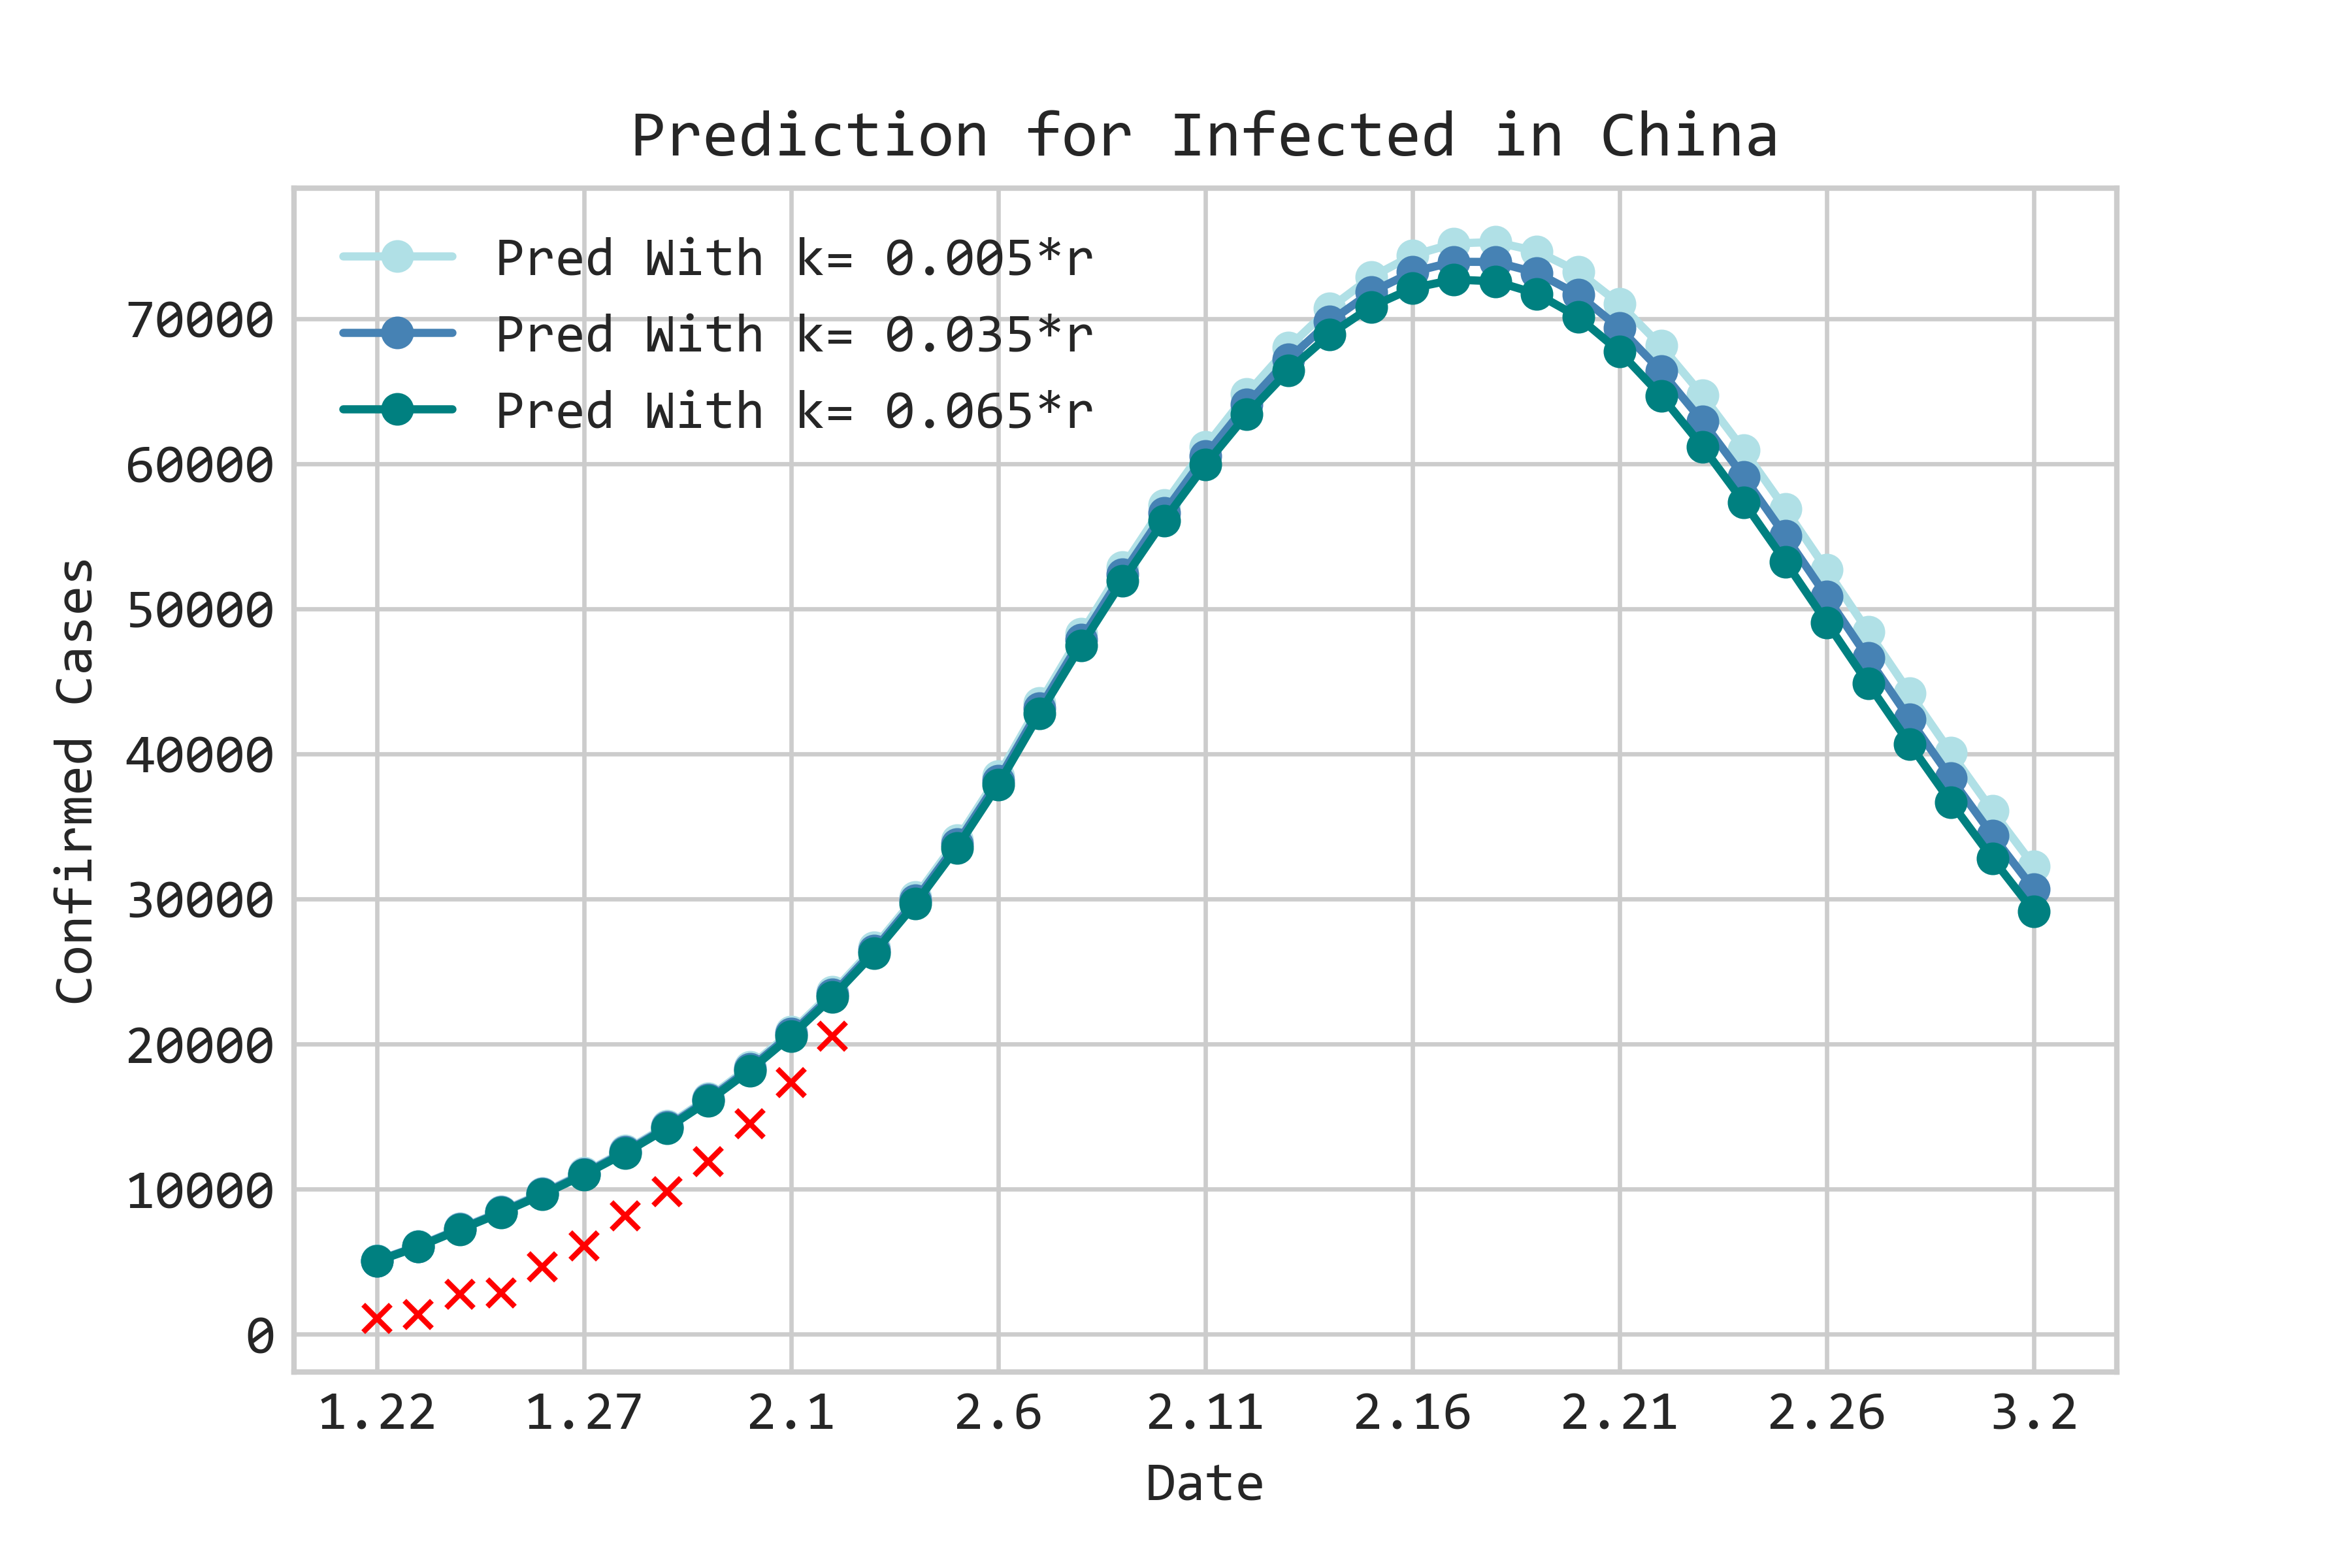
\includegraphics[width=1.0\textwidth]{053/figure/Sens_k.png}
        \caption{Sensitivity of $k$}
        \label{fig:Sens_k}
    \end{subfigure}
    \caption{Sensitivity Analysis}   \label{fig:Sens}
\end{figure}

\subsubsection{The Sensitivity of $\theta$ and $k$}
These two parameters do not appear in the expression of $R$. However, their sensitivities are in different orders of magnitude, as presented in Figure~\ref{fig:Sens_thita} and Figure~\ref{fig:Sens_k}. Numerically we have:
\begin{align*}
    S_{\theta}(\theta = 0.14) &= \frac{123000 - 40000}{0.16 - 0.12} \times \frac{0.14}{74000} \approx 3.93 \\
    S_k(k = 0.005) &= \frac{75000 - 72000}{(0.065 - 0.005) \times r} \times \frac{0.035 \times r}{74000} \approx 0.02
\end{align*}

We think that the reason for the huge difference in the sensitivities of these two parameters might be that increasing $\theta$ significantly accelerate the process of $E$ to $I$, and thus raise the chance of $S$ to $E$. However, as recovered and dead individuals are both removed from the chain of infection as the immunity is permanent, the rise of $k$ does nearly nothing to our prediction.

\subsection{Strengths and Weaknesses}
\subsubsection{Strengths}
\begin{enumerate}
    \item Collect plenty statistics from official source and make full use of them. Our data is mainly obtained from the Health Commission of a region or country, which has high credibility. With reliable and useful data, we can build, validate and apply our MoC-SEIR model confidently.
    \item Take various factors into consideration. To address the disadvantage of classic SEIR, we introduce several factors to our modified model, including population flow, secondary infection and the appearance of effective treatments, and quantify their impacts on the epidemic scenario. In this way, we successfully depict the spread process of 2019-nCoV and give some reasonable predictions to its trend with influences of different factors.
    \item Offer high value in application. Based on our analysis on the reproductive number, we propose many trains of thought to help prevent the virus spreading among crowds in different perspectives.
    \item Have flexibility and adaptability. Our model can adapt to the realistic situation better than the raw SEIR model and more parameters means a stronger expression ability.
\end{enumerate}

\subsubsection{Weaknesses}
\begin{enumerate}
    \item Some real conditions and exceptions are neglected. We simplify our model by only considering the outflow from Wuhan, while population flow between other regions might entangle the model a little bit. Also, the situation in some region has been interfered by accidental factors, which are ignored in our model.
    \item Lacking detailed oversea data and analysis. As the outbreak took place suddenly, there are few statistics and survey abroad. Therefore, we use grey prediction to forecast the trend out of China, failing to give concrete analysis.
    \item The robustness of our model is not very strong. As a common disadvantage of the models of infectious disease, the simulation result is highly correlated to some parameters, which ultimately changes $R_0$, as seen in our modified model.
    
\end{enumerate}

\section{Application}
As discussed in Section~\ref{Sec:Modeling} and Section~\ref{Sec:analysis}, we find several major factors having enormous impacts on the spread of virus, which provide us many useful trains of thought to protect ourselves and help to control virus spreading. Here we list and explain mathematically some of them.

\begin{itemize}
    \item \textbf{Supply enough test kits.} At the very beginning of the outbreak, there was huge scarcity of test tools which kind of led to potential carriers spreading virus everywhere. What's worse, the shortage could give us underestimation of the current situation and give rise to more fatalities.
    \item \textbf{A 14-days quarantine is still needed in both individual and collective scale.} The basic function of quarantine is to rule out the possibility of being potential carriers. It also cuts population flow and serves as a buffer against the reflow peek.
    \item \textbf{Decrease population density in public and cut population flow.} We have presented the direct impact on the epidemic situation of $a$ as it changes the basic reproductive number $R_0$. The reduction of population density and flow leads to a decline in $a$, which in turn lowers the reproductive number and inhibit the spread of virus. \textit{This might be realized mainly by Chinese government.}
    \item \textbf{Improve personal protection against virus.} This, obviously, is aimed at reducing $\gamma$, which has a similar effect as $a$. As we protect ourselves better, we would have a lower chance of being infected when staying close to infectious individuals. \textit{This might be done mainly by single person.}
    \item \textbf{Encourage the production of medical supplies and the researches on treatment.} Lastly there are ways to make $r$ higher. If infected people are cured more efficiently, then less healthy individuals might be infected. At the same time, the discovery of effective treatment, as shown in Section~\ref{subsubSec:treat}, can also help a lot to control and improve the situation. \textit{These might be accomplished by Chinese government, related enterprises and scientific research teams together.}
\end{itemize}
    
\section{Conclusion}
In this paper, we look deep into the development and trend of the epidemic situation of 2019-nCoV. We first present the simulation results of classic SEIR and then modify it with extra features taking the effect of population flow brought by traditional transportation and control measures taken by the Chinese government into consideration, which leads to the proposition of our \textbf{modified compartmental SEIR model}.

Based on our modified model, we give a prediction of domestic infections in the next period of time, which indicates that the increasing of newly infected individuals is about to stop by the end of February. \textbf{Grey Verhulst model} is then introduced to forecast oversea infections as few statistics and factors are known to us, suggesting the spread trend has been stemmed abroad. Next we quantify the effectiveness of Chinese government's measures by changing corresponding features in our model and look into their losses in the economic aspect. We speculate that the virus devastate the tertiary industry most for the Spring Festival is such a boon for the industry. Emergence of two types of powerful factors are also mathematically analyzed. In total, our conclusion is that WHO is expected to terminate the PHEIC in the end of March.

Measures, in either personal or national perspective, are fully discussed, which might reduce the chance of virus spread between individuals. In future works, the subtle influences of exposers and population variation can be explored. We hope our model offers an insight into what's happening in China and assist China CDC with making informed decisions. 
\newpage

\section{Blog}

\centerline{\Large{Five Key Ways to Combat 2019-nCov}}

The outbreak of Coronavirus has claimed over 500 lives and the number continues to climb. This time period is traditional Chinese new year when families get together and have a reunion dinner. The disaster pushes China into a economic downturn, industrial production stagnating and stores closed except those providing the basic life support and have something to with medicine.

Nonetheless, the Chinese government's prompt response and well management prevent the situation from getting worse. Here we will analyze some policies based on the result of our model and explain why some actions are recommended.

\begin{enumerate}
    \item $\textbf{Cites are increasingly going under lockdown.}$ On Jan. 23 The first city, Wuhan, declared to lock the city, stop running public transportation and limit the cars on the road, followed by other cities in Hubei. This policy played an indispensable role in preventing a broader outbreak. It also limits the inner spreading in cities by banning festival gatherings. By our calculation, the infectious has been cut up to 68\% due to these measures. So we recommend you to stay home and try to avoid go outside.
    \item $\textbf{Raise awareness across the public.}$ The Internet keeps people updated about the latest information about the virus and government's suggestions. Now almost everyone in the street wears a mask in China.  Besides, people outside Hubei make all the way to help this areas plagued by virus. The donations made by civilians actually ease the shortage of supplies in way. Here we advise not attending any gatherings wash hands and keep your house well-ventilated.
    \item  $\textbf{The virus is well tracked and early confirm cases are all linked to Wuhan.}$ This characteristic gives the Health Commission a clue and helps to locate the most potential carriers, those having been to Wuhan. Timely quarantine has been deployed and prevents more infection. If you know someone who has been to Wuhan or even Hubei, we suggest you to report to the community office or call 110 right now. If you just came back from Hubei or have been with guys from Hubei, it is necessary for you to have a 14-days quarantine for the sake of your family health.
    \item $\textbf{The unity and optimism prevails over adversity.}$ Over past 20 days, the outbreak has seen donations from people across the country to the areas plagued by virus. They send food, medical supplies and so on. Hospitals outside the Hubei dispatches medical team to ease the hospital staff shortage in Hubei. Hopefully, 
    the outbreak has been brought under control and a downturn is expected in the near future. 
    \item $\textbf{China has learned its lessons from the fight against SARS.}$ Now, hospitals are  equipped with more advanced facilities and better-trained doctors and have more accurate ways to detect the virus. Most of all, the Internet makes the information reachable for everyone and keeps us updated about latest developments which prevents the social panic. 
\end{enumerate}

Now, the fight against the plague has stepped into a crucial stage. Where the plague leads us to is determined by you, me and everyone in this country. Follow the instructions above and we as a nation will make through this devastating disaster.

\newpage
\printbibliography
\newpage

\begin{appendices}
\section{Grey Verhulst Model}
\lstinputlisting[language=Matlab]{code/GM_Verhust.m}
\section{Data Preprocessing}
\lstinputlisting[language=Python]{code/generate_province_data.py}
\section{SEIR Model}
\lstinputlisting[language=Python]{code/Prediction_For_Presentation.py}
\end{appendices}
\end{document}